% MathLedger Field Manual — Architect’s Notes
% This is a didactic companion to the whitepaper + research paper,
% written as a self-study lab manual for the project Sovereign.

\documentclass[11pt]{article}

% ---------- Encoding & Fonts ----------
\usepackage[utf8]{inputenc}
\usepackage[T1]{fontenc}
\usepackage{textcomp}

% ---------- Layout & Typography ----------
\usepackage[margin=0.5in, landscape]{geometry}
\usepackage{microtype}
\usepackage{parskip}   % space between paragraphs
\usepackage{setspace}
\onehalfspacing
\usepackage{titlesec}
\usepackage{enumitem}
\usepackage{booktabs}
\usepackage{csquotes}
\usepackage{longtable} % For better glossary tables
\usepackage{array}     % For better table column formatting
\emergencystretch=2em

% ---------- Fonts ----------
\usepackage[scaled]{helvet}
\usepackage{newpxtext,newpxmath}

% ---------- Math & Algorithms ----------
% newpx already defines \Bbbk and \openbox, so relax before AMS packages re-introduce them
\let\Bbbk\relax
\let\openbox\relax
\usepackage{mathtools,amssymb,amsthm,bm}
\usepackage{float}
\usepackage[ruled,vlined,linesnumbered]{algorithm2e}
\usepackage{listings}
\lstset{
  basicstyle=\ttfamily\small,
  columns=fullflexible,
  keepspaces=true,
  literate={∧}{{\ensuremath{\land}}}1
           {∨}{{\ensuremath{\lor}}}1
           {→}{{\ensuremath{\to}}}1
           {⟨}{{\ensuremath{\langle}}}1
           {⟩}{{\ensuremath{\rangle}}}1
}

% Theorem environments
\newtheorem{definition}{Definition}
\newtheorem{theorem}{Theorem}
\newtheorem{lemma}{Lemma}
\newtheorem{remark}{Remark}
\newtheorem{assumption}{Assumption}
\newtheorem{proposition}{Proposition}

% ---------- Graphics ----------
\usepackage{xcolor}
\definecolor{sec-blue}{RGB}{0, 50, 100}
\usepackage{graphicx}
\usepackage{caption}
\usepackage{tikz}
\usetikzlibrary{arrows.meta,positioning,fit,calc,shadows.blur,decorations.pathreplacing,shapes.geometric,shapes.misc,backgrounds}
\tikzset{
  base/.style={align=center, font=\sffamily\small, drop shadow, text=black},
  process/.style={base, rectangle, rounded corners=4pt, draw=blue!60!black, fill=blue!5, thick, minimum width=3.2cm, minimum height=1.4cm},
  datastore/.style={base, cylinder, shape border rotate=90, aspect=0.25, draw=orange!60!black, fill=orange!10, thick, minimum width=2.5cm, minimum height=1.8cm},
  config/.style={base, rectangle, chamfered rectangle, chamfered rectangle corners={north west, south east}, draw=purple!60!black, fill=purple!5, thick, minimum width=2.5cm, minimum height=1.2cm},
  line/.style={-Latex, thick, draw=black!70, rounded corners=4pt},
  label_text/.style={font=\footnotesize\sffamily, color=black!80, fill=white, inner sep=2pt}
}
\usepackage{pgfplots}
\pgfplotsset{compat=1.18}

% ---------- Links ----------
\usepackage[hidelinks]{hyperref}
\usepackage[capitalize]{cleveref}

% ---------- Meta Macros ----------
\newcommand{\system}{\textsc{MathLedger}}
\newcommand{\blockterm}{\ifmmode\mathsf{Block}\else\textsf{Block}\fi}
\newcommand{\ledger}{\ifmmode\mathsf{Ledger}\else\textsf{Ledger}\fi}
\newcommand{\hash}{\ifmmode\mathsf{hash}\else\textsf{hash}\fi}
\newcommand{\merkleroot}{\ensuremath{\mathrm{SHA256}}}
\newcommand{\concat}{\mathbin{\|}}
\newcommand{\Vnum}{\mathcal{V}_{\text{num}}}
\newcommand{\sectiondivider}{\par\medskip\hrule\medskip\par}

\DeclareMathOperator{\Hash}{Hash}
\newcommand{\E}{\mathbb{E}}
\newcommand{\1}{\mathbf{1}}

% ---------- Section Formatting ----------
\titleformat{\section}
  {\normalfont\Large\bfseries\color{sec-blue}}{\thesection}{1em}{}[{\titlerule[0.8pt]}]
\titlespacing*{\section}{0pt}{2.0ex plus 1ex minus .2ex}{1.0ex}
\titlespacing*{\subsection}{0pt}{1.5ex plus 1ex minus .2ex}{0.8ex}

% ============================================================
\begin{document}
\begin{center}
{\Huge \textbf{MathLedger Field Manual}}\\[0.5em]
{\Large An Architect's Guide to Reflexive Formal Learning}\\[0.75em]
{\large Internal Notes for Project Sovereign}\\[0.5em]
\today
\end{center}
\vspace{1em}

\begin{abstract}
\noindent
These notes are a self-study manual for \system{}, written from the perspective of an \emph{architect} rather than an implementer. The goal is to understand, in painstaking conceptual detail,
\begin{itemize}[leftmargin=1.5em]
  \item why current AI systems hallucinate and cannot be trusted as substrates for truth;
  \item how \system{} constructs a cryptographically-verifiable ledger of mathematical knowledge;
  \item how the \emph{Chain of Verifiable Cognition} is built: from user input to proof-or-abstain, to ledger attestation, to dual attestation, to Reflexive Formal Learning (RFL);
  \item how the whitepaper's architectural claims and the research paper's RFL convergence claims fit together;
  \item how the ``First Organism'' vertical slice and the Wide Slice abstention experiment operationalize these ideas in Phase~I.
\end{itemize}
The manual is intended to be read like a textbook and lab manual: some sections explain background theory, others walk through the \system{} architecture, and others connect the theory to concrete bottlenecks in the AI industry. The objective is \emph{command knowledge}: to be able to reason about the system as a whole, audit it, and explain it to serious technical stakeholders and potential acquirers.
\end{abstract}

\tableofcontents
\newpage

% ============================================================
\section*{0.\;Prerequisite Roadmap}
\addcontentsline{toc}{section}{0.\;Prerequisite Roadmap}
\label{sec:prereq}

This manual assumes you are comfortable reading technical documents but does \emph{not} assume you are already a specialist in logic, cryptography, or stochastic approximation. To study \system{} ``from the ground up,'' the recommended background is:

\begin{itemize}[leftmargin=1.5em]
  \item \textbf{Logic \& Proof Assistants (used in \cref{sec:logic,sec:curriculum}):}
  \begin{itemize}[leftmargin=1.5em]
    \item Propositional and first-order logic (syntax, semantics, soundness, completeness).
    \item Basic familiarity with proof assistants (e.g., Lean, Coq, Isabelle): how tactics assemble a proof term.
  \end{itemize}
  \item \textbf{Cryptography \& Data Structures (used in \cref{sec:crypto,sec:dual-attestation}):}
  \begin{itemize}[leftmargin=1.5em]
    \item Cryptographic hash functions, Merkle trees, collision resistance.
    \item Canonicalization of data (e.g., canonical JSON) and domain separation.
  \end{itemize}
  \item \textbf{Probability \& Stochastic Processes (used in \cref{sec:prob-sa,sec:rfl-conceptual,sec:rfl-dynamics}):}
  \begin{itemize}[leftmargin=1.5em]
    \item Random variables, expectations, conditional expectation.
    \item Filtrations, adapted sequences, and (super)martingales at a conceptual level.
    \item The high-level shape of stochastic approximation and convergence theorems.
  \end{itemize}
  \item \textbf{Topological Data Analysis (used in \cref{sec:tda-cognition,app:cortex}):}
\begin{itemize}[leftmargin=1.5em]
  \item Simplicial complexes, homology, Betti numbers.
  \item Persistent homology and stability under perturbations.
  \item Intuition for ridges, manifolds, and coherent structure in high-dimensional data.
\end{itemize}
This background is not required to operate \system{}, but is essential for understanding
Phase~III integrity mechanisms such as the TDA Mind Scanner.
  \item \textbf{Search, Planning, \& RL (used in \cref{sec:search}):}
  \begin{itemize}[leftmargin=1.5em]
    \item Tree/graph search, beam search, Monte Carlo planning.
    \item Basic reinforcement learning concepts: policy, value, exploration.
  \end{itemize}
  \item \textbf{Systems \& Data Engineering (used in \cref{sec:system-overview,sec:runbook}):}
  \begin{itemize}[leftmargin=1.5em]
    \item Relational schemas, HTTP APIs, background workers.
    \item Basic DevOps: configuration, jobs, logs, metrics.
  \end{itemize}
\end{itemize}

If any of these are unfamiliar:
\begin{itemize}[leftmargin=1.5em]
  \item You can read \cref{sec:logic,sec:crypto,sec:prob-sa} as targeted primers.
  \item \cref{sec:end-to-end} provides a concrete, end-to-end example; refer back to it as an anchor while reading.
  \item \cref{sec:glossary} summarizes symbols and terms for quick lookup.
\end{itemize}

The fastest way for a founder to get up to speed is:
\begin{enumerate}[leftmargin=1.5em]
  \item Read \cref{sec:orientation,sec:logic,sec:crypto} in order.
  \item Skim \cref{sec:prob-sa} to get the ``shape'' of RFL as a learning rule.
  \item Read \cref{sec:search,sec:system-overview,sec:curriculum,sec:dual-attestation}.
  \item Study \cref{sec:rfl-conceptual,sec:rfl-dynamics,sec:metabolism,sec:end-to-end}.
  \item Finish with \cref{sec:scaling-laws,sec:runbook,sec:industry,sec:use,sec:glossary}.
\end{enumerate}

% ============================================================
\section{Orientation: What MathLedger Is Solving}
\label{sec:orientation}

\subsection{The AI Bottleneck: Competence Without Trust}

Modern large language models (LLMs) are astonishingly capable pattern recognizers. They can emulate proofs, imitate experts, and generate code and explanations at scale. Yet they suffer from a structural defect:
they optimize for \emph{likelihood of text}, not \emph{truth of claims}. This produces:
\begin{itemize}[leftmargin=1.5em]
  \item \textbf{Hallucinations:} confident, fluent statements with no grounding in any underlying proof or mechanism.
  \item \textbf{Opaque reasoning:} even when an answer is correct, there is no auditable chain of inference.
  \item \textbf{Adversarial brittleness:} small prompt changes can flip answers without any semantic justification.
\end{itemize}

In safety-critical domains (finance, law, science, safety policy, infrastructure), this is unacceptable. The industry is discovering that:
\begin{quote}
  \emph{Performance without verifiability is not deployable at scale.}
\end{quote}

This is the core bottleneck: we do not just need models that \emph{answer}; we need systems that can \emph{justify}.

\subsection{Caveat: Reliability Does Not Remove the Need for Auditability}
\label{subsec:reliability-not-enough}

A common objection is that sufficiently capable systems will become reliable enough that formal provenance and verifiable cognitive history are unnecessary overhead.
This manual adopts the opposite engineering stance:

\begin{quote}
\emph{As system reliability increases, the marginal value of auditability does not go to zero; it typically increases.}
\end{quote}

The reason is structural. High-capability systems expand the action space and autonomy horizon.
When failures become rare, they also become harder to detect, harder to reproduce, and more consequential when they occur.
In such regimes, the operational problem shifts from ``reducing error rate'' to ``maintaining a verifiable record of what occurred, under which conditions, and why.''

\system{} therefore treats provenance as infrastructure rather than as a patch for low capability.
Even if task accuracy approaches a high ceiling, the Chain of Verifiable Cognition remains necessary for replay, accountability, dispute resolution, and long-horizon learning integrity.

\noindent\textit{This is an architectural claim about observability, not a claim about any specific model family.}

\subsection{The MathLedger Thesis}

\system{} attacks this bottleneck by moving from a statistical substrate to a \emph{formal} and \emph{cryptographic} substrate:
\begin{itemize}[leftmargin=1.5em]
  \item All reasoning is expressed in a formal language (Lean).
  \item All proofs are checked by a small, trustworthy kernel.
  \item All successful proofs (and abstentions) are recorded into a \emph{monotone ledger} of mathematical truths.
  \item All user interactions (queries, confirmations, corrections) are hashed into a parallel UI-Merkle structure.
  \item A dual-attestation layer braids these into a single composite root $H_t$, the \emph{epistemic fingerprint} of an epoch.
  \item A \emph{Reflexive Formal Learning} (RFL) loop uses these verified events as the only learning signal for policy updates.
\end{itemize}

The whitepaper describes the architecture; the research paper provides a mathematical model of the learning dynamics. These notes sit \emph{between} them: they are meant to give you an intuitive and structural understanding of each piece.

\subsection{Architect’s Checklist: Non-Negotiables}
\label{subsec:architect-checklist}

When you are ``in the pocket'' as architect, there are a handful of invariants you must never lose sight of. They are the short list you carry into every design review, debugging session, and investor call.

\begin{enumerate}[leftmargin=1.5em]
  \item \textbf{Canonical identity is sacred.}\\
  Every mathematical object (statement, proof, UI event) has:
  \begin{itemize}[leftmargin=1.5em]
    \item a \emph{normalization} $\mathcal{N}(\cdot)$ (logic-aware, not just string sorting);
    \item a canonical encoding $\mathcal{E}(\mathcal{N}(\cdot))$;
    \item a domain-separated hash $\hash(\cdot)$ built on top.
  \end{itemize}
  No code is allowed to bypass this path. If something appears in the ledger, it must have come through canonical normalization and hashing.

  \item \textbf{The ledger is monotone and cryptographically sealed.}\\
  Blocks are append-only. The set of verified statements only grows. Each block $B_t$ is committed to by a Merkle root $R_t$; changing any proof or statement after the fact changes $R_t$, and thus invalidates the block.

  \item \textbf{Dual attestation binds machine and human cognition.}\\
  Each epoch $t$ has:
  \begin{itemize}[leftmargin=1.5em]
    \item $R_t$: reasoning Merkle root over proofs;
    \item $U_t$: UI Merkle root over user events;
    \item $H_t = \Hash(\texttt{"EPOCH:"}\concat R_t\concat U_t)$: the composite root.
  \end{itemize}
  $H_t$ is the \emph{only} scalar you are allowed to use as the ``fingerprint'' of an epoch. Any story about an epoch that does not pass through $(R_t,U_t,H_t)$ is incomplete.

  \item \textbf{First Organism is the vertical slice, not the whole organism.}\\
  The First Organism pipeline:
  \[
    \text{UI Event} \to \text{Curriculum Gate} \to \text{Derivation} \to \text{Lean Abstention} \to \text{Dual Attest } H_t \to \text{RFL}
  \]
  is your \emph{Phase~I closure test}. It answers: “Can we run one fully hermetic, deterministic cycle end-to-end, with a recomputable $H_t$ and a non-trivial abstention pattern?” It is not meant to solve all of alignment; it is meant to prove the pipeline works.

  \item \textbf{RFL is stochastic approximation on epistemic risk.}\\
  At the conceptual level:
  \[
    X_t = \mathcal{J}(\pi_t) = \Pr[\mathcal{V}(e_t)\neq 1],
  \]
  and the update
  \[
    \pi_{t+1} = \pi_t \oplus \eta_t \Phi(\mathcal{V}(e_t),\pi_t)
  \]
  is a noisy descent step on $X_t$. The details live in \cref{sec:rfl-dynamics}, but the core intuition is:
  \begin{quote}
    \emph{Policies that cause fewer failures and abstentions become more likely; policies that cause them become less likely.}
  \end{quote}

  \item \textbf{Phase~I vs.\ Phase~II are quarantined.}\\
  \begin{itemize}[leftmargin=1.5em]
    \item Phase~I experiments (First Organism, Wide Slice abstention dynamics) assume an ideal verifier and hermetic environment.
    \item Phase~II experiments (imperfect verifier, noisy Lean, broader capability metrics) are explicitly \emph{out of scope} for Phase~I claims.
  \end{itemize}
  This quarantine is a feature: it lets you speak with ``Sober Truth'' about what is actually demonstrated.

  \item \textbf{Wide Slice experiments probe learning, not just plumbing.}\\
  The Wide Slice configuration is chosen such that:
  \begin{itemize}[leftmargin=1.5em]
    \item the problem class is non-trivial (abstentions are initially frequent);
    \item the slice still runs under realistic budgets;
    \item RFL can, in principle, learn to reduce abstentions over many cycles.
  \end{itemize}
  The goal is not to maximize proofs-per-second; it is to observe whether $A_{\mathrm{rfl}}(t)$ drops relative to $A_{\mathrm{base}}(t)$ under a fixed slice, as described in \cref{sec:scaling-laws}.
\end{enumerate}

If you remember nothing else, remember these invariants. Everything else in this manual is an elaboration.

% ============================================================
% --- Added per Layer-3 Narrative Alignment (2025-12-13)
\section{System Positioning: Layer-3 Infrastructure}
\label{sec:layer-3-positioning}

\system{} is Layer-3 infrastructure. It is neither a user-facing application (Layer 1) nor a proof-generation engine (Layer 2). Its role is to provide a neutral, verifiable substrate that records the outputs of other systems.

The AI-driven mathematics ecosystem can be understood as a three-layer stack:
\begin{itemize}[leftmargin=1.5em]
    \item \textbf{Layer 1: The Human Layer.} Mathematicians, scientists, engineers, and auditors who pose queries, interpret results, and make decisions.
    \item \textbf{Layer 2: The Engine Layer.} AI models, theorem provers, and symbolic search algorithms that generate formal artifacts (e.g., proof candidates, formalizations, refutations).
    \item \textbf{Layer 3: The Ledger Layer.} A system of record that provides immutable provenance, causal ordering, and cryptographic attestation for the artifacts produced by Layer 2.
\end{itemize}

\system{} occupies Layer 3 exclusively. It is the flight data recorder, not the pilot or the engine. It records what happened, when it happened, and under what conditions, making the entire process auditable and reproducible. It does not compete with proof generators; it provides the infrastructure to make their outputs trustworthy at scale.

\subsection{Canonical Product Narratives}
\label{subsec:product-narratives}

The system's role can be described from different perspectives, each emphasizing a different facet of its utility. These are not different products; they are frames for understanding a single, unified system.

\paragraph{Academic Frame.}
\system{} is an audit-grade ledger that records the provenance, ordering, and reproducibility of formally verified proofs, making large-scale machine-assisted mathematics inspectable rather than opaque.

\paragraph{Defense / Governance Frame.}
\system{} provides tamper-evident provenance and causal ordering for AI reasoning artifacts, enabling post-hoc auditability, replay, and accountability without interfering with system operation.

\paragraph{Universal Frame.}
\system{} is the provenance infrastructure for AI reasoning—recording what happened, in what order, and under which conditions, so complex cognitive systems can be audited at scale.

These frames do not imply different capabilities. They are narrative lenses that adapt the same core functionality—immutable, verifiable recording—to the concerns of different stakeholders, from research integrity to regulatory compliance.

% ============================================================
\section{Why the Name \system{} Still Holds}
\label{sec:name-doctrine}


\subsection{The Original Meaning: A Ledger of Mathematical Truth}


The name \system{} originally referred to a specific and deliberately narrow ambition:
to construct a cryptographically verifiable, append-only ledger of mathematical truths,
derived from first principles and checked by a small, trusted proof kernel (Lean).


In its earliest conception, \system{} was anchored to:
\begin{itemize}[leftmargin=1.5em]
  \item a curriculum ladder over formal theories (beginning with propositional logic);
  \item proof objects as first-class artifacts;
  \item canonical normalization and hashing of statements and proofs;
  \item a monotone ledger recording only verified results (or explicit abstentions).
\end{itemize}


This was not branding convenience. Mathematics was chosen because it is the domain in which
\emph{truth is unambiguous}, verification is decidable (within bounded theories), and
formal error is intolerable. Mathematics was the \emph{training ground} in which the core
epistemic commitments of the system could be made explicit and non-negotiable.


\subsection{What Changed: From Mathematical Truth to Verifiable Cognition}


As the system evolved, it became clear that the original insight generalized:


\begin{quote}
\emph{If you can build a ledger of mathematical truth, you can build a ledger of cognition itself.}
\end{quote}


The same primitives that make a mathematical fact trustworthy also make a reasoning process
trustworthy:
\begin{itemize}[leftmargin=1.5em]
  \item canonical representation,
  \item formal verification (or principled abstention),
  \item cryptographic commitment,
  \item replayability and audit.
\end{itemize}


What expanded was not the abandonment of mathematics, but the \emph{domain of application}.
The ledger no longer records only theorems; it records:
\begin{itemize}[leftmargin=1.5em]
  \item verified proofs and abstentions,
  \item policy-relevant reasoning events,
  \item user-confirmed or corrected interactions,
  \item stability and coherence signals over reasoning trajectories.
\end{itemize}


In other words, the object of record shifted from
\[
\text{``mathematical statements''}
\quad\longrightarrow\quad
\text{``formally attested acts of reasoning.''}
\]


\subsection{The Name as a Constraint, Not a Limitation}


The name \system{} persists because it encodes a \emph{constraint}, not a scope limitation.


Calling the system a ``ledger'' commits it to:
\begin{itemize}[leftmargin=1.5em]
  \item immutability,
  \item append-only semantics,
  \item explicit provenance,
  \item third-party verifiability.
\end{itemize}


Calling it ``math'' commits it to:
\begin{itemize}[leftmargin=1.5em]
  \item formal semantics rather than heuristics,
  \item proof-or-abstain rather than plausible output,
  \item kernel-checked correctness rather than statistical confidence.
\end{itemize}


These commitments remain binding even as the system expands to govern learning dynamics,
agentic behavior, and self-modifying policies. Any component that cannot be reduced to
formal objects with canonical identity and verifiable semantics is, by definition,
\emph{out of scope} for the ledger.


In this sense, the name \system{} functions as a guardrail: it prevents the system from
quietly drifting into informal, unverifiable, or purely statistical regimes.


\subsection{The Math Ladder Was Not Abandoned; It Was Generalized}


The original capability ladder—PL $\rightarrow$ FOL $\rightarrow$ richer theories—was never
discarded. It was elevated to a more general abstraction:


\begin{quote}
\emph{Mathematics is the first domain in which verifiable cognition is demonstrated,
not the last domain in which it applies.}
\end{quote}


The early Lean-based slices remain the canonical proof that:
\begin{itemize}[leftmargin=1.5em]
  \item the ledger semantics are sound,
  \item canonicalization is non-negotiable,
  \item abstention is a first-class outcome,
  \item learning can be driven by verification rather than reward proxies.
\end{itemize}


Everything built on top of \system{}—RFL, USLA, TDA-based integrity monitoring—inherits these
constraints. They do not replace the mathematical foundation; they rely on it.


\subsection{Architect’s Interpretation}


An architect should read the name \system{} as follows:
\begin{quote}
\emph{This system treats cognition with the same standards that mathematics demands of truth.}
\end{quote}


The ledger is no longer merely a catalog of theorems. It is a permanent, cryptographically
sealed record of what a reasoning system has proven, abstained from, and learned—under
formal rules that do not change with scale, fashion, or capability.


The name remains accurate because the system never relaxed its original promise.
It simply discovered that the promise applied more broadly than first imagined.

% ============================================================
\section{Uncharted Surface Area \& The Phase-II Critical Path}
\label{sec:uncharted}

This section records the major domains of \system{} that remain unexplored or only lightly touched. Its purpose is architectural clarity: to prevent overextension, avoid premature parallelism, and to highlight the minimal set of bottlenecks that must be solved before scaling beyond Phase~I.

The following list is compressed, technical, and non-narrative by design. It is the ``surface area map'' of the organism.

\subsection{1.\;Uncharted or Underdetailed Domains}

\textbf{(1) Statement Language Beyond PL:}\\
FOL signatures (arity tables); term rewriting semantics; congruence closure specifics; quantifier-instantiation heuristics; Skolemization/Herbrand truncation; equality-reasoning performance bounds.

\textbf{(2) Proof Object Canonicalization:}\\
Canonical Lean proof-term encoding (AST→bytes); tactic-trace normalization; canonical proof compression; deterministic subproof ordering; schema evolution across Lean versions.

\textbf{(3) Statement Graph Analytics:}\\
Structural clustering; lemma-kernel detection; DAG metrics (centrality, reuse); proof-zippering; curriculum-level pruning.

\textbf{(4) Block \& Ledger Economics:}\\
Proof–cost weighting; block-size economics; censorship resistance; replay protection; multi-writer protocols.

\textbf{(5) Proof DAG Compression:}\\
Merkle-DAG hybrids; subproof dedupe; structural sharing; canonical topo-ordering; block-size impact.

\textbf{(6) Long-Horizon Policy Representations:}\\
Policy features; representing local proof states; serializing policies for long-term RFL; drift control; rollback safety.

\textbf{(7) ML Training Infrastructure:}\\
Dataset schema; canonical train/val/test splits; augmentation rules; slice-boundary ablations; determinism constraints.

\textbf{(8) Inter-Slice Generalization:}\\
Cross-slice transfer; difficulty calibration; overfitting detection; PL-to-FOL generalization properties.

\textbf{(9) Imperfect Verifier Regime (Phase~II):}\\
Lean noise models; timeout nondeterminism; mixed verifier tiers; statistical filtering; RFL robustness under $\varepsilon_v>0$.

\textbf{(10) Protocol-Level Safety Guarantees:}\\
Replay analysis; canonical JSON evolution; schema versioning; DoS vectors; malformed-data handling; rollback protocol.

\textbf{(11) Multi-Agent Coordination:}\\
Cross-prover dedupe; attested provenance in multi-agent settings; conflict resolution.

\textbf{(12) UI Verified Input at Scale:}\\
Event-schema versioning; spam filtering; UX for non-experts; trust-weighted corrections.

\textbf{(13) Block Replay \& Historical Audit:}\\
Full ledger replay; historical root verification; forensic tooling; long-term snapshots.

\textbf{(14) Privacy \& Confidentiality:}\\
ZK-validity proofs; private commitments; selective disclosure; redactable blocks.

\textbf{(15) Distributed Ledger Backends:}\\
Sharded proof storage; distributed Merkle proofs; local-first replicas; trustless verification.

\textbf{(16) Epistemic Metrics Beyond Abstention:}\\
Policy entropy; proof-complexity spectra; difficulty frontier; ladder success profiles; RFL energy landscape.

\textbf{(17) Non-PL Theories: Algebra, Geometry, Analysis:}\\
Canonical languages for algebraic structures; algebraic-normalization rules; SMT-witness integration; numeric certificates.

\textbf{(18) Semantic Telemetry for Proof Attempts:}\\
Tactic-pattern extraction; symbolic embeddings; telemetry schema; error-pattern discovery.

\textbf{(19) Governance / Consensus / Permissions:}\\
Write-permissions; provenance signatures; governance for schema evolution.

\textbf{(20) Disaster Recovery / Durability:}\\
Cold storage; cross-region replication; reconstruction from proofs; checkpointing policy states.

\subsection{2.\;Tier Classification: What Is Pressing for Phase~II}

Not all twenty domains are equally urgent. Only five are \textbf{blocking} for the Phase~I~$\to$~Phase~II transition. The remainder depend on these foundations and should not be opened prematurely.

\paragraph{Tier~1 (Pressing \& Blocking).}
\begin{itemize}[leftmargin=2em]
  \item \textbf{Imperfect Verifier Handling}: nondeterminism, noise models, mixed verifier tiers.
  \item \textbf{ML Policy Representation \& Training Infrastructure}: embeddings, canonical datasets, determinism.
  \item \textbf{Proof-Term Canonicalization}: stable AST→bytes, canonical traces, versioning.
  \item \textbf{Proof DAG Compression \& Deduplication}: block-size control; deterministic topo-order.
  \item \textbf{Attestation Privacy \& Schema Hardening}: versioning, replay protection, UI-event privacy.
\end{itemize}

\paragraph{Tier~2 (Important but Non-Blocking).}
Block economics; multi-agent coordination; slice-transfer theory; distributed backends; advanced theories; telemetry; DR.

\paragraph{Tier~3 (Future Roadmap).}
World-of-truth interfaces; axiom-system explorers; semantic truth atlas; humanities integration.

\subsection{3.\;Architect’s Directive: The Iron-Triangle Critical Path}

Phase~II requires concentration, not expansion. The organism is not bottlenecked by parallelism; it is bottlenecked by:
\begin{itemize}[leftmargin=2em]
  \item determinism,
  \item canonicalization,
  \item correctness constraints,
  \item RFL stability under noise.
\end{itemize}

The architect’s minimal allocation is:
\begin{enumerate}[leftmargin=2em]
  \item \textbf{The Sentinel}: canonicalization, hash-law correctness, proof-term stability.
  \item \textbf{The Stabilizer}: imperfect-verifier models, noise-robust RFL, determinism enforcement.
  \item \textbf{The Architect}: ML policy schema, dataset canonicalization, neuro-symbolic interface.
\end{enumerate}

These three domains form the \emph{Phase-II critical path}. Only once they stabilize is it safe to open Tier~2 or Tier~3 domains.

% ============================================================
\section{Governed Cognitive Substrates: The Nation-State Analogy}
\label{sec:cognitive-nation-state}

\subsection{Why a ``Nation-State'' Analogy Emerged Organically}

As \system{} evolved through canonicalization, dual attestation, the ledger, RFL, USLA,
and the TDA Mind Scanner, a surprising but structurally precise analogy emerged:
\begin{quote}
\emph{\system{} behaves like a governed nation-state in the space of cognition.}
\end{quote}

This is not a political analogy but a structural one. Each subsystem of \system{} plays
a role isomorphic to classical components of a stable constitutional order:

\begin{center}
\renewcommand{\arraystretch}{1.2}
\begin{tabular}{p{0.28\linewidth} p{0.62\linewidth}}
\toprule
\textbf{MathLedger Component} & \textbf{Nation-State Structural Role} \\
\midrule
Canonicalization + Hash Law & Constitutional definition of identity; census of objects \\
Monotone Ledger ($R_t$)     & Historical archive / judiciary record \\
UI Root ($U_t$)             & Democratic input / public record \\
Dual Attestation ($H_t$)    & Binding law linking state action and public input \\
USLA (Unified System Law)   & Constitutional physics: the lawful evolution of state \\
Invariants (INV-001--008)   & Non-negotiable constitutional guarantees \\
CDI Defects (CDI-001--010)  & Diagnosed failure modes of governance \\
Safe Region $\Omega$        & Lawful operating domain of the state \\
TDA Mind Scanner (HSS)      & Structural integrity auditor / stability ministry \\
RFL                         & Policy evolution mechanism; legislative-amendment engine \\
Shadow Mode                 & Judicial review / simulation before enactment \\
\bottomrule
\end{tabular}
\end{center}

\subsection{Three Kinds of ``Revolution'' in Cognitive Systems}

Human political revolutions do \emph{not} map directly into cognitive substrates.
However, dynamical systems admit three structural transitions that resemble
``regime change'' at the mathematical level:

\paragraph{1.\;Phase Transition (Constitutional Upgrade).}
Introduction of a new system law, invariant, or topology constraint that reorganizes the
entire governance system. Examples in \system{}:
\begin{itemize}[leftmargin=1.5em]
  \item introduction of USLA,
  \item activation of invariants in Phase~IX,
  \item deployment of the TDA Mind Scanner,
  \item establishing the safe region $\Omega$.
\end{itemize}

\paragraph{2.\;Regime Collapse (Attractor Failure).}
A violation of stability conditions causes the system to fall into a pathological
attractor (e.g.\ CDI-010: fixed-point multiplicity collapse). This is the analogue of a
state failure, not a political uprising. USLA + invariants are engineered to prevent this.

\paragraph{3.\;Regime Renewal (Constitutional Amendment).}
Safe, deliberate updates to thresholds, sensitivities, invariants, or curriculum pacing.
These correspond to lawful ``reforms'' rather than upheavals.

\subsection{Why Political Uprisings Have No Analogue in \system{}}

Political revolutions rely on:
\begin{itemize}[leftmargin=1.5em]
  \item multiple heterogeneous agents with conflicting incentives,
  \item resource scarcity,
  \item emotional contagion,
  \item decentralized coordination,
  \item asymmetric information,
  \item breakdown of institutional trust.
\end{itemize}

None of these mechanisms exist in \system{}:
\begin{itemize}[leftmargin=1.5em]
  \item There is a single policy vector $\pi_t$, not a population of competing agents.
  \item Resources (budgets) are not subject to competition or inequality.
  \item All information is canonicalized and attested.
  \item Governance is mathematically defined, not socially negotiated.
  \item Stability is enforced by invariants, USLA, and TDA coherence.
\end{itemize}

Thus, \emph{Arab Spring–style phenomena are not meaningful failure modes} in cognitive
substrates. The closest analogue is a USLA-detectable divergence leading to a controlled
rollback.

\subsection{Phase Transitions as ``Cognitive Regime Changes''}

We record the major constitutional epochs of \system{}:

\begin{enumerate}[leftmargin=1.5em]
  \item \textbf{Epoch I: Correctness Regime}  
        Proof-or-abstain; monotone ledger; dual attestation.
  \item \textbf{Epoch II: Stability Regime}  
        USLA state vector ($x\in\mathbb{R}^{15}$), safe region $\Omega$, HARD gate.
  \item \textbf{Epoch III: Structural Regime}  
        TDA Mind Scanner; SNS/PCS/DRS → HSS; topological governance.
  \item \textbf{Epoch IV: Meta-Learning Regime}  
        RFL with topology-gated updates; self-stabilizing adaptation loops.
  \item \textbf{Epoch V: Governance Hardening (Future)}  
        Advisory→Active transition; rollback procedures; constitutional freeze boundaries.
\end{enumerate}

Each epoch represents a “governance realignment,” not a political revolution.

\subsection{Architect’s Interpretation: A Governed Cognitive Commonwealth}

Combining the ledger, RFL, USLA, and TDA yields a cognitive substrate with:

\begin{itemize}[leftmargin=1.5em]
  \item \textbf{Law (USLA)}, 
  \item \textbf{History (Ledger)}, 
  \item \textbf{Public Input (UI root)}, 
  \item \textbf{Structural Integrity Agency (TDA)}, 
  \item \textbf{Policy Mechanism (RFL)}, 
  \item \textbf{Judicial Replay (Lean)}, 
  \item \textbf{Shadow Review (Simulator)}.
\end{itemize}

This is a \emph{self-governing cognitive commonwealth}:  
a symbolic organism whose stability is maintained through formal constitutional
mechanisms rather than human sociopolitical dynamics.

\begin{quote}
\textbf{Truth is the judiciary.  
Topology is the internal affairs bureau.  
USLA is the constitution.  
RFL is the legislature.  
The ledger is the national archive.}
\end{quote}

This structural analogy clarifies how \system{} scales safely into Phase~III and beyond.

% ============================================================
\section{Background I: Logic, Proof, and Semantics}
\label{sec:logic}

This section is not a Lean tutorial. It is a conceptual primer so that you, as architect, can reason about:
\begin{itemize}[leftmargin=1.5em]
  \item what a statement is,
  \item what it means to be \emph{true},
  \item how a proof assistant differs from an LLM.
\end{itemize}

\subsection{Syntax vs.\ Semantics}

\begin{definition}[Syntax and Semantics]
A \emph{syntax} is a formal language: a set of symbols and formation rules that tell you which strings are well-formed formulas (WFFs). \emph{Semantics} assign meanings (truth values) to formulas, typically via models or valuations.
\end{definition}

An LLM is primarily a syntactic engine: it knows what \emph{looks} like a plausible string, or proof, or paper. A proof assistant such as Lean is concerned with semantics: a statement is only accepted if it is derivable from axioms in a sound proof system.

\subsection{Soundness and Completeness}

\begin{definition}[Soundness]
A proof system is \emph{sound} if every statement it can prove is semantically true in all models.
\end{definition}

\begin{definition}[Completeness]
A proof system is \emph{complete} if every semantically true statement (in a given class of models) is provable in the system.
\end{definition}

For \system{}:
\begin{itemize}[leftmargin=1.5em]
  \item Soundness is non-negotiable: anything claimed as proven in the ledger must be \emph{true} under the formal semantics.
  \item Completeness is not required (and, by Gödel, not fully attainable in rich theories). The ledger can abstain: if it cannot prove something, it simply does not record it.
\end{itemize}

This is where the proof-or-abstain doctrine comes from:
\begin{quote}
  \emph{It is better to abstain than to accept a false proof.}
\end{quote}

\subsection{Propositional Logic and Tautologies}

In the early phases (PL slices), statements live in propositional logic:
variables $p,q,r,\dots$ connected by logical operators $\land,\lor,\rightarrow,\lnot$.

\begin{definition}[Tautology]
A formula is a \emph{tautology} if it is true under every valuation of its propositional variables.
\end{definition}

Tautologies correspond to algebraic invariants of truth; they are foundational for bootstrapping a ledger of basic logical facts.

% ============================================================
\section{Background II: Cryptography and Ledgers}
\label{sec:crypto}

\subsection{Hash Functions and Canonical Identity}

A cryptographic hash function $h$ takes arbitrary data and produces a fixed-length fingerprint:
\begin{itemize}[leftmargin=1.5em]
  \item It is hard to find two different inputs with the same hash (collision resistance).
  \item It is hard to find an input with a given target hash (preimage resistance).
\end{itemize}

In \system{}, we define a canonical identity for statements:

\begin{definition}[Canonical Identity]
Let $\mathcal{N}(s)$ be a normalization of formula $s$ (NNF, commutative sorting, right-association). Let $\mathcal{E}$ encode the normalized abstract syntax tree (AST) into bytes. Then:
\[
  \hash(s) \coloneqq \merkleroot(\mathcal{E}(\mathcal{N}(s))).
\]
\end{definition}

Normalization ensures that semantically equivalent formulas get the same hash, regardless of superficial syntactic variation.

\subsection{Merkle Trees and Monotone Ledgers}

A Merkle tree commits to a set of leaf values by recursively hashing pairs. This is used to define block roots.

\begin{definition}[Monotone Ledger]
A ledger $\ledger$ is a sequence of blocks $(B_1,B_2,\dots)$ where each $B_t$:
\begin{enumerate}[label=(\roman*),leftmargin=1.5em]
  \item Contains proofs of previously unseen statements (by $\hash$).
  \item Records verification status in Lean.
  \item Has a Merkle root $R_t$ computed over sorted proof IDs.
\end{enumerate}
The ledger is \emph{monotone} if the set of recorded statements only grows:
\[
  \bigcup_{i\le t} B_i \subseteq \bigcup_{i\le t+1} B_i\quad\text{for all }t.
\]
\end{definition}

This gives you a \emph{financial-grade} audit trail of mathematical truths.

\subsection{Canonicalization and Domain Separation}

Hashing ``raw'' data is dangerous. The same bytes may be interpreted in multiple ways; different logical objects may accidentally collide as byte sequences. Architecturally, we use:
\begin{itemize}[leftmargin=1.5em]
  \item \textbf{Canonical serialization:} statements, proofs, events, and blocks are encoded using fixed, versioned formats:
  \begin{itemize}[leftmargin=1.5em]
    \item canonical JSON (RFC 8785-style normalization) for API-visible objects;
    \item deterministic AST encodings for internal proof and statement structures;
    \item explicit field ordering and UTF-8 normalization everywhere.
  \end{itemize}
  \item \textbf{Domain separation:} different kinds of objects get distinct prefixes before hashing. For example:
  \[
    \Hash_{\text{stmt}}(s) = \Hash(\texttt{"STMT:"}\concat \mathcal{E}(\mathcal{N}(s))),
  \]
  \[
    \Hash_{\text{proof}}(p) = \Hash(\texttt{"PROOF:"}\concat \mathcal{E}(p)),
  \]
  \[
    \Hash_{\text{ui}}(e) = \Hash(\texttt{"UI:"}\concat \mathcal{E}(e)).
  \]
\end{itemize}

Domain separation ensures that no UI event can be misinterpreted as a proof, and vice versa, even if the underlying bytes happen to match.

\subsection{Threat Model (Informal)}

At a high level, the adversary may:
\begin{itemize}[leftmargin=1.5em]
  \item read and replay messages on the network;
  \item attempt to tamper with DB records, logs, or block headers;
  \item attempt to fabricate proofs or UI events after the fact.
\end{itemize}

We assume:
\begin{itemize}[leftmargin=1.5em]
  \item the hash function behaves like a random oracle for our purposes;
  \item the Lean kernel and canonicalization code are trusted (or at least auditable);
  \item the adversary cannot break collision resistance at the scale of our deployments.
\end{itemize}

Under these assumptions:
\begin{itemize}[leftmargin=1.5em]
  \item tampering with any statement/proof/event after it has been sealed into a block will change the Merkle root;
  \item tampering with UI events will change $U_t$ and thus $H_t$;
  \item replay attacks are detectable via nonces, timestamps, and sequence numbers in the canonical encodings.
\end{itemize}

\subsection{Post-Quantum Threat Model and Migration Path}
\label{subsec:post-quantum}

From an architect’s perspective, quantum computing introduces two classes of risk:

\begin{itemize}[leftmargin=1.5em]
  \item \textbf{Asymmetric primitives:} RSA, classical Diffie–Hellman, and standard ECC are vulnerable to Shor-type attacks, collapsing their long-term security.
  \item \textbf{Symmetric primitives:} Grover-type attacks effectively halve the security level of a $k$-bit key (brute force drops from $2^k$ to about $2^{k/2}$ work).
\end{itemize}

\paragraph{Where \system{} sits today.}
\begin{itemize}[leftmargin=1.5em]
  \item Hashing and Merkle trees are built on top of classical symmetric primitives (e.g.\ SHA-256).
  \item No hard dependency on RSA/ECC appears in the core ledger semantics (signatures or TLS may be used at the transport layer but are not part of the \emph{semantics} of blocks).
\end{itemize}

This means:
\begin{itemize}[leftmargin=1.5em]
  \item \textbf{Ephemeral security:} For the near term, 256-bit hash-based commitments are sufficient even under a Grover-style reduction.
  \item \textbf{Archival security:} For very long-lived ledgers (``100-year proofs''), we should assume that future quantum adversaries may eventually mount stronger attacks.
\end{itemize}

\paragraph{Post-quantum migration sketch.}
Without committing to specific schemes, the architect-level plan is:
\begin{enumerate}[leftmargin=1.5em]
  \item \textbf{Abstract the hash primitive.} Treat $\Hash(\cdot)$ as a logical interface with parameters $(\texttt{alg\_id}, \texttt{digest})$, not a hard-coded SHA-256 string.
  \item \textbf{Introduce versioned hash domains.} Extend domain separation with an explicit algorithm/version tag:
  \[
    \Hash_{\text{stmt}}^{(v)}(s) = \Hash^{(v)}\bigl(\texttt{"STMT:"}\concat \mathcal{E}(\mathcal{N}(s))\bigr),
  \]
  where $v\in\{\texttt{sha256},\texttt{pq\_hash\_1},\dots\}$.
  \item \textbf{Dual-commitment transition.} For a transitional period, commit each block header under both:
  \begin{itemize}[leftmargin=1.5em]
    \item legacy hash $\Hash^{(\texttt{sha256})}(R_t\concat U_t)$,
    \item post-quantum candidate $\Hash^{(\texttt{pq})}(R_t\concat U_t)$.
  \end{itemize}
  This preserves backward compatibility while seeding future verifiers with quantum-safe roots.
  \item \textbf{Signature layer abstraction.} If/when block-level signatures or provenance attestations are added, design them behind a generic ``signature scheme'' interface so that classical schemes can be swapped for post-quantum ones (hash-based, lattice-based, etc.) without touching ledger semantics.
  \item \textbf{Canon freeze, not algorithm freeze.} The canonical encodings of statements, proofs, and events must be frozen; the hash \emph{algorithm} that digests those encodings is allowed to evolve in a versioned way.
\end{enumerate}

\paragraph{Design principle.}
The field manual stance is:

\begin{quote}
\emph{Canonical form is forever; cryptographic algorithms are replaceable.}
\end{quote}

Your job as architect is to ensure that:
\begin{itemize}[leftmargin=1.5em]
  \item canonical encodings $\mathcal{E}(\mathcal{N}(\cdot))$ are quantum-agnostic and stable;
  \item the ledger supports multiple hash/attestation algorithms side-by-side via explicit versioning;
  \item a later ``quantum-hardening'' phase can be executed without invalidating the existing chain of verifiable cognition.
\end{itemize}

\subsection{(Informal) Quantum-Resilient Invariants}

Even in a future with powerful quantum hardware, the following invariants should remain true if the migration path is followed:
\begin{itemize}[leftmargin=1.5em]
  \item A block’s canonical content is reconstructible from its canonical encodings and the (versioned) hash function.
  \item A third party can verify an historical $H_t$ by using the appropriate algorithm ID and canonical encodings.
  \item Dual attestation semantics (binding between $R_t$ and $U_t$) remain unchanged; only the cryptographic primitive wrapping them may change.
\end{itemize}

% ============================================================
\section{Background III: Probability \& Stochastic Approximation}
\label{sec:prob-sa}

This section provides just enough probability and stochastic approximation to make RFL in \cref{sec:rfl-conceptual,sec:rfl-dynamics} intelligible.

\subsection{Random Variables, Filtrations, and Adapted Processes}

\begin{definition}[Random Variable]
A random variable $X$ is a measurable function from an underlying sample space $\Omega$ to some state space (e.g.\ $\mathbb{R}$). Intuitively, $X(\omega)$ is the numeric outcome when the world is in state $\omega$.
\end{definition}

\begin{definition}[Filtration]
A \emph{filtration} $(\mathcal{F}_t)_{t\ge 0}$ is a sequence of $\sigma$-algebras
\[
  \mathcal{F}_0 \subseteq \mathcal{F}_1 \subseteq \mathcal{F}_2 \subseteq \dots
\]
representing the information revealed up to time $t$.
\end{definition}

\begin{definition}[Adapted Process]
A sequence of random variables $(X_t)_{t\ge 0}$ is \emph{adapted} to $(\mathcal{F}_t)$ if each $X_t$ is measurable with respect to $\mathcal{F}_t$. Intuitively: $X_t$ only depends on information revealed up to time $t$.
\end{definition}

In \system{}, we will treat:
\begin{itemize}[leftmargin=1.5em]
  \item $\mathcal{F}_t$: everything the system knows up to epoch $t$ (ledger, policies, logs, etc.).
  \item $X_t$: a quantity derived from the current policy $\pi_t$ (e.g.\ epistemic risk $\mathcal{J}(\pi_t)$).
\end{itemize}

\subsection{Martingales and Supermartingales (Intuition)}

\begin{definition}[Supermartingale (informal)]
A sequence $(X_t)$ adapted to $(\mathcal{F}_t)$ is a \emph{supermartingale} if:
\[
  \E[X_{t+1}\mid \mathcal{F}_t] \le X_t
\]
for all $t$.
\end{definition}

Intuition:
\begin{itemize}[leftmargin=1.5em]
  \item A martingale has constant conditional expectation ($=$).
  \item A supermartingale has non-increasing conditional expectation ($\le$).
\end{itemize}

If $X_t$ is nonnegative and forms a supermartingale, it tends not to grow; under mild conditions, it converges almost surely to a finite limit.

\subsection{A Toy Robbins–Siegmund-Type Result}

We will not prove it here, but the rough shape of a Robbins--Siegmund convergence statement is:

\begin{quote}
  Let $(X_t)$ be a nonnegative adapted process. Suppose there exist nonnegative adapted $(Y_t)$ and $(Z_t)$ such that
  \[
    \E[X_{t+1} \mid \mathcal{F}_t] \le X_t - Y_t + Z_t,
  \]
  and that $\sum_t Z_t < \infty$ almost surely. Then:
  \begin{itemize}
    \item $\sum_t Y_t < \infty$ almost surely,
    \item $X_t$ converges almost surely to a finite random variable $X_\infty$.
  \end{itemize}
\end{quote}

Informally: if the expected decrement $Y_t$ dominates the noise $Z_t$ and the noise is summable, then the process cannot keep decreasing indefinitely; it must converge.

\subsection{Scalar Toy Example}

Let $X_{t+1} = X_t - \alpha_t (X_t - \xi_t)$, where:
\begin{itemize}[leftmargin=1.5em]
  \item $\alpha_t \in (0,1)$ is a step size with $\sum_t \alpha_t = \infty$ and $\sum_t \alpha_t^2 < \infty$;
  \item $\xi_t$ is a bounded noise term with $\E[\xi_t \mid \mathcal{F}_t]=0$.
\end{itemize}
Then a classical result shows that $X_t$ converges to $0$ almost surely. You can view $X_t$ as a noisy, diminishing step toward zero, and the step-size conditions ensure that you move quickly enough (sum diverges) but noise is controlled (squares sum converges).

\subsection{Connection to RFL}

In \cref{sec:rfl-dynamics}, we will:
\begin{itemize}[leftmargin=1.5em]
  \item define a process $X_t = \mathcal{J}(\pi_t)$, the epistemic risk under policy $\pi_t$;
  \item show informally that $X_t$ satisfies a Robbins--Siegmund-type inequality:
  \[
    \E[X_{t+1} \mid \mathcal{F}_t] \le X_t - Y_t + Z_t,
  \]
  where $Y_t$ reflects expected risk reduction and $Z_t$ collects noise terms;
  \item argue that under mild assumptions, $X_t$ converges.
\end{itemize}

You do not need the full proof to reason as architect; you only need the shape: RFL is a noisy descent process on a well-defined notion of risk.

% ============================================================
\section{Search, Planning, and Event Generation}
\label{sec:search}

RFL acts on \emph{events} $e_t$. This section explains where those events come from.

\subsection{From Policy to Event Distribution}

At a high level:
\begin{itemize}[leftmargin=1.5em]
  \item The search/planner receives:
  \begin{itemize}[leftmargin=1.5em]
    \item a query or curriculum slice description (what to prove);
    \item the current policy $\pi_t$ (how to prioritize search);
    \item resource budgets (time, memory, beam width).
  \end{itemize}
  \item It runs a controlled search (graph/tree) over proof states.
  \item Each attempted proof, success, or abstention is an \emph{event} $e_t$.
\end{itemize}

Thus, the policy $\pi_t$ induces a distribution over events $e_t$ via the search dynamics.

\subsection{Planner Shape: Guided Graph Search}

We can view the prover as a guided search over a proof graph:
\begin{itemize}[leftmargin=1.5em]
  \item \textbf{State $s$:} a frontier configuration (current goals, context, partial proof tree).
  \item \textbf{Actions $a \in A(s)$:} apply a rule, tactic, or lemma at (part of) $s$.
  \item \textbf{Policy $\pi_t(a\mid s)$:} a scoring function that ranks actions by promise.
\end{itemize}

The planner maintains a frontier of states and repeatedly:
\begin{enumerate}[leftmargin=1.5em]
  \item selects a state $s$ from the frontier;
  \item samples or selects top-$k$ actions $a$ according to $\pi_t(a\mid s)$;
  \item expands resulting states until either:
  \begin{itemize}[leftmargin=1.5em]
    \item a proof is found and passes verification; or
    \item resources are exhausted and the attempt is marked \texttt{ABSTAIN}.
  \end{itemize}
\end{enumerate}

\subsection{RL, Exploration, and RFL}

There are two conceptually distinct learning mechanisms:
\begin{itemize}[leftmargin=1.5em]
  \item \textbf{RL-style learning:} reward-based updates for $\pi_t$ grounded in search success (e.g.\ proofs found, depth reached). This resembles standard policy-gradient or bandit-style learning.
  \item \textbf{RFL updates:} symbolic, verification-driven updates that treat $\mathcal{V}(e_t)\in\{1,0,\bot\}$ as the fundamental signal. Here $\bot$ represents abstention.
\end{itemize}

Operationally:
\begin{itemize}[leftmargin=1.5em]
  \item The same pipeline collects events $e_t$ with:
  \[
    e_t = \bigl(\text{slice}, \text{state/action trace}, \mathcal{V}(\text{attempt})\bigr).
  \]
  \item RL methods might optimize throughput or depth for a fixed slice.
  \item RFL methods treat $\mathcal{V}$ as the primitive and adjust $\pi_t$ only in directions that reduce epistemic risk (false positives and unnecessary abstentions).
\end{itemize}

As architect, you should think of RL as ``local performance tuning,'' while RFL enforces a global, verification-anchored learning law.

\subsection{Algorithmic Sketch: Event Generation Loop}

\begin{algorithm}[H]
\DontPrintSemicolon
\SetAlgoLined
\SetKwInOut{Input}{input}\SetKwInOut{Output}{output}
\Input{policy $\pi_t$, slice description $\mathcal{S}$, budgets $\mathcal{B}$}
\Output{event log $\mathcal{E}_t = \{e_1,\dots,e_n\}$}
\BlankLine
Initialize frontier with root states defined by $\mathcal{S}$\;
\While{resources in $\mathcal{B}$ remain}{
  select state $s$ from frontier (e.g.\ by depth or priority)\;
  compute candidate actions $A(s)$\;
  score actions using $\pi_t(\cdot\mid s)$ and select top-$k$\;
  \ForEach{$a \in \text{selected}$}{
    expand to new state $s'$; update frontier accordingly\;
    \If{goal reached or proof candidate $p$ assembled}{
      run verifier ladder on $p$ with budgets $\mathcal{B}$\;
      record event $e = \langle \mathcal{S}, s,a,p,\mathcal{V}(p)\rangle$ into $\mathcal{E}_t$\;
      \If{$\mathcal{V}(p)=1$}{persist proof $\&$ statement; possibly close branch}
    }
  }
}
\Return $\mathcal{E}_t$\;
\caption{Search / Planner Event Generation}
\end{algorithm}

The RFL loop in \cref{sec:rfl-dynamics} consumes these events $\mathcal{E}_t$.

% ============================================================
\section{System Overview: Organs of the Organism}
\label{sec:system-overview}

This section rephrases the whitepaper architecture in ``box-and-arrow'' language. You should be able to redraw this on a whiteboard and label what data moves on each arrow.

\subsection{Core Pipeline}

\begin{figure}[H]
\centering
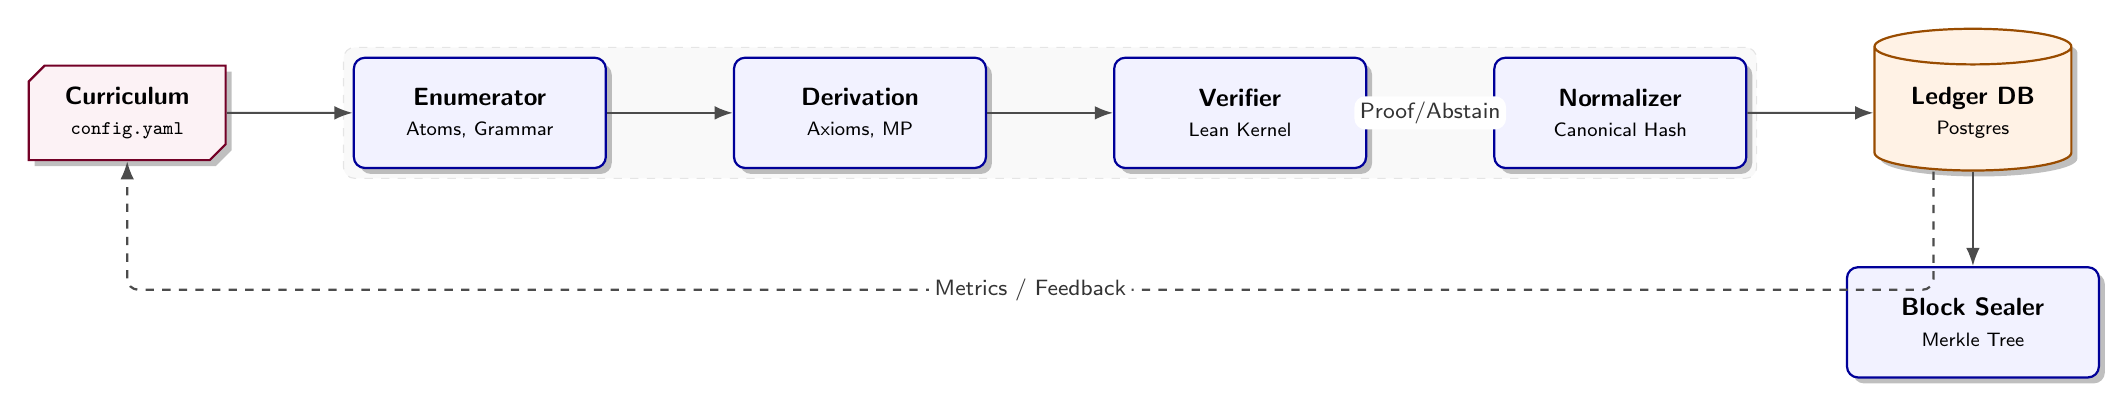
\begin{tikzpicture}[node distance=1.2cm and 1.6cm]
  % Nodes
  \node[config] (yaml) {\textbf{Curriculum}\\\scriptsize \texttt{config.yaml}};
  \node[process, right=of yaml] (enum) {\textbf{Enumerator}\\\scriptsize Atoms, Grammar};
  \node[process, right=of enum] (derive) {\textbf{Derivation}\\\scriptsize Axioms, MP};
  \node[process, right=of derive] (lean) {\textbf{Verifier}\\\scriptsize Lean Kernel};
  \node[process, right=of lean] (canon) {\textbf{Normalizer}\\\scriptsize Canonical Hash};
  \node[datastore, right=of canon] (db) {\textbf{Ledger DB}\\\scriptsize Postgres};
  \node[process, below=of db] (blocks) {\textbf{Block Sealer}\\\scriptsize Merkle Tree};

  % Edges
  \draw[line] (yaml) -- (enum);
  \draw[line] (enum) -- (derive);
  \draw[line] (derive) -- (lean);
  \draw[line] (lean) -- node[label_text]{Proof/Abstain} (canon);
  \draw[line] (canon) -- (db);
  \draw[line] (db) -- (blocks);

  % Feedback Loop
  \draw[line, dashed] (db.south) ++(-0.5,0) coordinate(dbs) -- ++(0,-1.5) -| (yaml.south) node[pos=0.25, label_text, fill=white] {Metrics / Feedback};
  
  % Background
  \begin{scope}[on background layer]
    \node[fit=(enum)(derive)(lean)(canon), rounded corners, fill=gray!5, draw=gray!20, dashed] {};
  \end{scope}
\end{tikzpicture}
\caption{Core Pipeline: From curriculum parameters to immutable ledger blocks.}
\end{figure}

\subsection{Data Model Intuition}

The core tables (conceptually):
\begin{itemize}[leftmargin=1.5em]
  \item \texttt{statements}: logical formulas, normalized, with $\hash(s)$ as primary identity.
  \item \texttt{proofs}: proof objects with fields such as prover, method, duration, status, transcript hash.
  \item \texttt{dependencies}: edges in the proof DAG (which proof depends on which statements).
  \item \texttt{blocks}: batches of proofs, with Merkle roots $R_t$.
  \item \texttt{runs}: operational metadata per run of the derivation engine / RFL.
\end{itemize}

Your mental model: the ledger is a big, append-only DAG of reasoning, with blocks providing cryptographic checkpoints.

\subsection*{Addendum: Topological Structure of Proof DAGs}
\addcontentsline{toc}{subsection}{Addendum: Topological Structure of Proof DAGs}

The global proof DAG maintained by \system{} is not merely a dependency graph; it is a
\emph{topological object}. Many structural properties of the organism---lemma reuse,
concept emergence, proof-strategy divergence, and reasoning degeneracy---manifest as
changes in the topology of local subgraphs.

In preparation for Phase~III, each local proof DAG $G=(V,E)$ can be lifted to a
\emph{simplicial complex} $K_{\mathrm{comb}}$ (a flag complex), by treating cliques in the
undirected 1-skeleton of $G$ as simplices. Cycles in $H_1(K_{\mathrm{comb}})$ correspond to
nontrivial reuse patterns or logical ``loops''; fragmentation in $H_0$ indicates instability
or degeneracy in reasoning. These constructions power the TDA Mind Scanner defined in
Appendix~C.

In short: the DAG is the ``visible anatomy,'' but its simplicial complex is the
``structural geometry.'' Both will be essential for understanding drift, stability, and
emergent behavior as RFL scales.

% ============================================================
\section{The Logic Ladder and Curriculum Slices}
\label{sec:curriculum}

\subsection{Curriculum as a Control Surface}

The curriculum ladder formalizes how the system climbs from simple theories to more complex ones.

At the bottom: propositional logic (PL). Above: FOL with equality, equational theories, linear arithmetic.

Each rung is not a monolithic theory, but a set of \emph{slices}:
bounded combinations of atom counts, formula depth, search budgets, etc.

\begin{definition}[Slice]
A \emph{slice} is a tuple of parameters:
\[
  (\text{atoms}, \text{depth}, \text{breadth}, \text{total}, \text{timeout}, \dots)
\]
governing enumeration and derivation for a constrained subspace of formulas.
\end{definition}

The curriculum specifies:
\begin{itemize}[leftmargin=1.5em]
  \item which slices exist per theory;
  \item what coverage / throughput / abstention thresholds they must meet before the system is allowed to ratchet upward.
\end{itemize}

\subsection{Authentic Synthetic Data}

Rather than scraping human-written proofs from the internet, \system{} generates its own statements within these slices and proves them (or abstains). This yields:
\begin{itemize}[leftmargin=1.5em]
  \item infinite data (the space of formulas grows combinatorially),
  \item with perfect provenance (every statement has a known hash and proof path),
  \item and tunable difficulty (via slice parameters).
\end{itemize}

For your purposes: the ladder is the “training curriculum” for the organism.

% ============================================================
\section{Dual Attestation and User-Verified Input}
\label{sec:dual-attestation}

\subsection{Reasoning Root and UI Root}

The ledger attests to the machine’s reasoning via $R_t$; the UI layer attests to human interaction via $U_t$.

\begin{definition}[Dual Attestation]
Let $R_t$ be the Merkle root over proof IDs in block $t$ (reasoning stream). Let $U_t$ be the Merkle root over UI events in the same epoch (user stream). Define the composite root:
\[
  H_t = \Hash(\texttt{"EPOCH:"}\concat R_t \concat U_t),
\]
binding what was \emph{thought} to what was \emph{asked/confirmed}.
\end{definition}

This is the basis of the \emph{Chain of Verifiable Cognition}:
every epoch $t$ has a cryptographic fingerprint $H_t$ that commits to both reasoning and UI.

Conceptually, within an epoch you may also track per-step roots (for fine-grained audit):
\begin{itemize}[leftmargin=1.5em]
  \item $r_\tau$: Merkle root over reasoning events at time-step $\tau$;
  \item $u_\tau$: Merkle root over UI events at time-step $\tau$;
  \item these feed into $R_t$ and $U_t$ via higher-level Merkle constructions.
\end{itemize}

\subsection{User-Verified Input Loop (UVIL)}

The UI is not just a front-end; it is part of the epistemic circuit.

\begin{definition}[User-Verified Input Loop]
Each user interaction is encoded as an event
\[
  \tau = \langle \texttt{actor},\ \texttt{kind}\in\{\text{confirm},\text{correct},\text{abstain}\},\ \texttt{target\_hash},\ \texttt{meta} \rangle
\]
and enters the UI-Merkle structure. The UVIL is the process by which these events are:
\begin{enumerate}[leftmargin=1.5em]
  \item normalized and recorded;
  \item referenced by $U_t$ and hence by $H_t$;
  \item later available as evidence in RFL updates and audits.
\end{enumerate}
\end{definition}

The key concept: human judgment is not “soft feedback”; it becomes a first-class, cryptographically-attested part of the substrate.

% ============================================================
\section{Trust Classes and Cryptographic Commitment}
\label{sec:trust-classes}

MathLedger does not attempt to collapse all forms of correctness, validation, or judgment into a single notion of ``truth.'' Instead, it explicitly distinguishes \emph{trust classes}: categories of artifacts differentiated by the strongest verification mechanism applicable to them.

This distinction is not cosmetic. It is fundamental to governance, auditability, and long-term system integrity.

\subsection{Trust Classes}

Each artifact recorded by MathLedger belongs to exactly one trust class:

\begin{itemize}
  \item \textbf{Formally Verified}: Artifacts whose correctness is established by a small, trusted kernel (e.g., Lean). These include formal statements and proof objects.
  \item \textbf{Mechanically Validated}: Artifacts whose correctness can be established by deterministic computation, tests, or certificates (e.g., recomputation, constraint checking).
  \item \textbf{Procedurally Attested}: Artifacts whose trust derives from provenance, authorization, or process (e.g., who approved what, under which authority).
  \item \textbf{Advisory}: Interpretive or heuristic outputs (e.g., narrative analyses, recommendations) that are explicitly not formally or mechanically verified.
\end{itemize}

These trust classes are intentionally non-interchangeable. A formally verified artifact is not ``more correct'' in a metaphysical sense; it is correct in a strictly narrower, explicitly defined domain.

\subsection{Separation of Verification and Attestation}

MathLedger enforces a strict separation between:
\begin{itemize}
  \item \emph{Verification} (establishing correctness relative to a formal system or checker), and
  \item \emph{Attestation} (recording intent, context, and provenance).
\end{itemize}

This separation prevents category errors such as treating interpretive judgments as formal truths or retroactively upgrading the trust status of an artifact.

\subsection{Cryptographic Commitment to Trust Class}

To prevent post hoc relabeling or misrepresentation, each artifact's trust class is included in the canonical serialization that is hashed into the ledger.

Concretely, each Merkle leaf commits to:
\[
\Hash(\texttt{trust\_class} \concat \texttt{artifact\_kind} \concat \texttt{artifact\_digest} \concat \texttt{checker\_id} \concat \texttt{checker\_version} \concat \ldots)
\]

This ensures that:
\begin{itemize}
  \item trust class is immutable once recorded,
  \item cryptographic integrity binds verification level to artifact content,
  \item future auditors cannot reinterpret an artifact under a stronger trust class than originally justified.
\end{itemize}

\subsection{Merkle Roots and Dual Attestation}

Let:
\begin{itemize}
  \item $R_t$ denote the Merkle root over verified or mechanically validated artifacts produced during epoch $t$,
  \item $U_t$ denote the Merkle root over human-facing intent, approvals, and contextual metadata.
\end{itemize}

The dual attestation root is defined as:
\[
H_t = \Hash(\texttt{epoch} \concat R_t \concat U_t)
\]

This construction binds formally checked results to the intent and context under which they were produced, without conflating correctness with authorization.

\subsection{Design Implication}

By explicitly typing trust and committing it cryptographically, MathLedger achieves two goals simultaneously:
\begin{enumerate}
  \item Maximal rigor where formal verification is possible.
  \item Honest accountability where it is not.
\end{enumerate}

This allows the system to extend beyond mathematics while remaining governance-safe, audit-friendly, and epistemically modest.

% ============================================================
\section{Reflexive Formal Learning (RFL): Conceptual Layer}
\label{sec:rfl-conceptual}

Now we shift from architecture to dynamics.

\subsection{Policies and Epistemic Risk}

Let $\Pi$ denote the space of reasoning policies (e.g., search heuristics, beam allocation, lemma selection strategies). Let $\pi_t \in \Pi$ be the policy at time $t$.

Each policy induces a distribution over \emph{events} $e_t$ (attempted proofs, abstentions) via the planner in \cref{sec:search}.

\begin{definition}[Epistemic Risk]
Given a verification function $\mathcal{V}(e)\in\{1,0,\bot\}$ (pass, fail, abstain), define the numeric surrogate
\[
  \Vnum(e) = \1\{\mathcal{V}(e)\neq 1\} \in \{0,1\}.
\]
Then the \emph{epistemic risk} of a policy is
\[
  \mathcal{J}(\pi) = \E_{e\sim P_\pi}[\Vnum(e)] = \Pr_{e\sim P_\pi}[\mathcal{V}(e)\neq 1],
\]
the probability that an event under policy $\pi$ is \emph{not} a verified success.
\end{definition}

Interpretation: $\mathcal{J}(\pi)$ is the mass of “error or abstention” events. RFL seeks to drive this down over time.

\subsection{Update Algebra}

RFL does not use gradients directly. It uses symbolic updates.

\begin{definition}[Update Algebra]
Let $\Delta\Pi$ be the space of symbolic policy deltas. Let $\oplus$ be an operation such that for any $\pi\in\Pi$ and $\Delta\in\Delta\Pi$:
\[
  \pi' = \pi \oplus \Delta
\]
is the updated policy. Assume a norm $\|\cdot\|_\Delta$ on $\Delta\Pi$ and a Lipschitz-like compatibility:
\[
  \|\pi\oplus\Delta - \pi\| \le L_\oplus \|\Delta\|_\Delta.
\]
\end{definition}

The RFL update law is:
\[
  \pi_{t+1} = \pi_t \oplus \eta_t \Phi(\mathcal{V}(e_t), \pi_t),
\]
where:
\begin{itemize}[leftmargin=1.5em]
  \item $\Phi$ maps the verification outcome and current policy to a delta in $\Delta\Pi$;
  \item $\eta_t$ is a stepsize.
\end{itemize}

Intuition: $\Phi$ is the symbolic analogue of “gradient direction” and $\eta_t$ is a learning rate. We will link this to stochastic approximation in \cref{sec:rfl-dynamics}.

\subsection{Abstention Notions}

It is useful to distinguish:
\begin{itemize}[leftmargin=1.5em]
  \item \textbf{Verifier-level abstain:} the Lean/SMT ladder timed out or could not construct a proof under budget; $\mathcal{V}(e)=\bot$.
  \item \textbf{System-level ABSTAIN:} even if the verifier succeeded, something in dual attestation or security checks failed, and the system refuses to serve an answer.
  \item \textbf{Policy-level abstention:} the planner chooses not to attempt certain branches or classes of queries at all, based on learned risk.
\end{itemize}

In RFL, $\Vnum(e)$ treats all non-verified events as ``bad'' (either failure or abstention). Later refinements can separate these categories more finely.

\subsection*{Addendum: RFL Requires Structural Integrity Signals}
\addcontentsline{toc}{subsection}{Addendum: RFL Requires Structural Integrity Signals}

RFL ensures that the policy $\pi_t$ evolves to reduce epistemic risk, but it does not
constrain the \emph{shape} of the internal reasoning that produces events.
It is possible---especially under long horizons or meta-learning---for policies to produce
logically sound outputs while drifting into degenerate internal modes: trivial proofs,
oscillatory reasoning, or unstable conceptual manifolds.

To address this, Phase~III introduces a structural integrity signal based on
\emph{Topological Data Analysis (TDA)}. For each event $e_t$, the TDA Mind Scanner
constructs simplicial complexes over local proof DAGs and metric filtrations over
reasoning trajectories. It produces a scalar Hallucination Stability Score (HSS) that
quantifies coherence:
\[
\mathrm{HSS}(e_t) \in [0,1].
\]
RFL updates become gated not only by $\mathcal{V}(e_t)$ but also by HSS, ensuring that
learning is anchored in both \emph{correctness} (Lean) and \emph{structural stability}
(Topology). See Appendix~C.

% ============================================================
\section{RFL: From Architecture to Dynamics}
\label{sec:rfl-dynamics}

We now connect the conceptual RFL picture to the stochastic-approximation background in \cref{sec:prob-sa}.

\subsection{Defining the Process}

Let:
\begin{itemize}[leftmargin=1.5em]
  \item $\mathcal{F}_t$ be the filtration generated by all events and random choices up to time $t$: policies, events, ledger updates, etc.
  \item $\pi_t$ be $\mathcal{F}_t$-adapted (the policy at time $t$ depends only on past information).
  \item $X_t = \mathcal{J}(\pi_t)$ be the epistemic risk under $\pi_t$.
\end{itemize}

The RFL update:
\[
  \pi_{t+1} = \pi_t \oplus \eta_t \Phi(\mathcal{V}(e_t), \pi_t)
\]
induces a stochastic process $\{X_t\}$ adapted to $\{\mathcal{F}_t\}$.

\subsection{Noise and Descent}

At a high level, we expect:
\[
  \E[X_{t+1} \mid \mathcal{F}_t] \le X_t - Y_t + Z_t,
\]
where:
\begin{itemize}[leftmargin=1.5em]
  \item $Y_t$ captures expected risk reduction from successful updates (e.g.\ moving probability mass away from high-risk actions);
  \item $Z_t$ captures noise terms (stochasticity in event sampling, approximations, imperfect feedback).
\end{itemize}

Under mild assumptions:
\begin{itemize}[leftmargin=1.5em]
  \item $X_t \ge 0$ always (it is a probability);
  \item $\sum_t Z_t < \infty$ almost surely (noise is controlled);
  \item step sizes $\eta_t$ satisfy $\sum_t \eta_t = \infty$ and $\sum_t \eta_t^2 < \infty$.
\end{itemize}
we are in the regime where a Robbins--Siegmund-type theorem applies, yielding:
\begin{itemize}[leftmargin=1.5em]
  \item $\sum_t Y_t < \infty$ almost surely;
  \item $X_t$ converges almost surely to a finite limit.
\end{itemize}

As architect, you do not need to memorize the theorems, but you \emph{do} need to understand the invariants:
\begin{itemize}[leftmargin=1.5em]
  \item $X_t$ measures epistemic risk;
  \item each update is a small, noisy step meant to reduce $X_t$;
  \item dual attestation and the ledger ensure that $\mathcal{V}(e_t)$ is trustworthy, so $X_t$ is meaningful.
\end{itemize}

\subsection{High-Level Takeaway}

RFL is not ``magic math.'' It is:
\begin{itemize}[leftmargin=1.5em]
  \item a stochastic approximation procedure on a well-defined loss $\mathcal{J}$;
  \item with a constrained update algebra (symbolic deltas via $\oplus$);
  \item powered by a verifier-based oracle $\mathcal{V}$ secured by the ledger and dual attestation.
\end{itemize}

Once you see it that way, you can reason about it using the same mental tools you use for SGD or policy gradient, with the twist that the signal is proof-or-abstain rather than real-valued reward.

\subsection*{Addendum: Topological Stability as a SA-Friendly Signal}
\addcontentsline{toc}{subsection}{Addendum: Topological Stability as a SA-Friendly Signal}

Stochastic approximation theory requires the learning signal to be reliable, bounded, and
well-behaved under noise. While $\mathcal{V}(e_t)$ meets these criteria, it is inherently
sparse: most events are failures or abstentions. In contrast, topological quantities
derived from reasoning trajectories yield \emph{continuous}, SA-compatible signals.

The long-lifetime components of persistent homology (see Appendix~C) yield a stability
score PCS that varies smoothly with changes in policy and search geometry. Coupled with
SNS (proof complexity) and DRS (distance from reference topology), the composite HSS
provides a scalar that integrates seamlessly into the SA framework:
\[
\pi_{t+1} = \pi_t \oplus \eta_t \, \Phi\bigl(\mathcal{V}(e_t), \mathrm{HSS}(e_t), \pi_t\bigr).
\]
This yields a two-axis descent: correctness pressure from $\mathcal{V}$ and coherence
pressure from topology. The theory remains intact because HSS is bounded and can be made
Lipschitz with respect to the policy under mild assumptions.

% ============================================================
\section{Organism Metabolism: Cross-Layer Flow}
\label{sec:metabolism}

This section gives the ``one-page metabolism'' of \system{}: who consumes what, and what they excrete.

\subsection{Metabolism Diagram}

\begin{figure}[H]
\centering
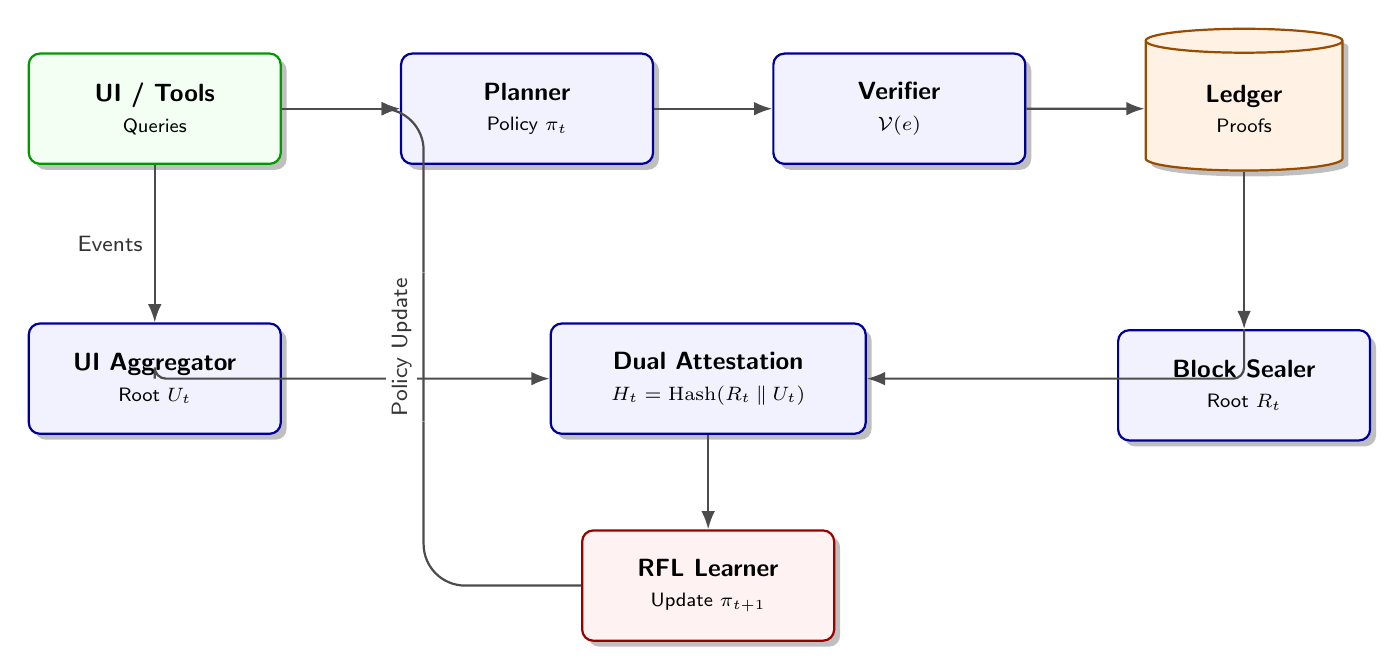
\begin{tikzpicture}[node distance=1.5cm and 1.5cm]
  % Top Row: Action
  \node[process, fill=green!5, draw=green!60!black] (ui) {\textbf{UI / Tools}\\\scriptsize Queries};
  \node[process, right=of ui] (planner) {\textbf{Planner}\\\scriptsize Policy $\pi_t$};
  \node[process, right=of planner] (verifier) {\textbf{Verifier}\\\scriptsize $\mathcal{V}(e)$};
  \node[datastore, right=of verifier] (db) {\textbf{Ledger}\\\scriptsize Proofs};

  % Bottom Row: Attestation
  \node[process, below=2cm of ui] (uiagg) {\textbf{UI Aggregator}\\\scriptsize Root $U_t$};
  \node[process, below=2cm of db] (sealer) {\textbf{Block Sealer}\\\scriptsize Root $R_t$};
  
  % Center Convergence
  \node[process, below=2cm of planner, xshift=2.3cm, minimum width=4cm] (dual) {\textbf{Dual Attestation}\\\scriptsize $H_t = \Hash(R_t \concat U_t)$};
  
  % Bottom: Learning
  \node[process, below=1.2cm of dual, fill=red!5, draw=red!60!black] (rfl) {\textbf{RFL Learner}\\\scriptsize Update $\pi_{t+1}$};

  % Edges
  \draw[line] (ui) -- (planner);
  \draw[line] (planner) -- (verifier);
  \draw[line] (verifier) -- (db);
  
  \draw[line] (ui) -- node[midway, left, xshift=-2pt, label_text] {Events} (uiagg);
  \draw[line] (db) -- (sealer);
  
  \draw[line] (uiagg) |- (dual);
  \draw[line] (sealer) |- (dual);
  
  \draw[line] (dual) -- (rfl);
  
  % RFL Feedback Loop - Wide left side
  \draw[line, rounded corners=15pt] (rfl.west) -- ++(-2.0,0) coordinate(turn1)
       -- node[midway, rotate=90, above, yshift=2pt, label_text] {Policy Update} (turn1 |- planner.west)
       -- (planner.west);

\end{tikzpicture}
\caption{Metabolism: The cycle of user interaction, verification, attestation, and learning.}
\end{figure}

\subsection{Component Table}

\begin{center}
\renewcommand{\arraystretch}{1.15}
\begin{tabular}{p{0.18\linewidth} p{0.32\linewidth} p{0.32\linewidth}}
\toprule
\textbf{Component} & \textbf{Consumes} & \textbf{Produces} \\
\midrule
UI / Tools &
User queries, ledger references &
UI events, prompts, corrections \\
Planner / Search &
Queries, slices, policy $\pi_t$ &
Attempted proofs, traces $e_t$ \\
Verifier Ladder &
Proof candidates, budgets &
Verification outcomes $\mathcal{V}(e)$ \\
Ledger DB &
Verified proofs, statements &
Block candidates, metrics \\
Block Sealer &
Proof IDs, run metadata &
Block headers, $R_t$ \\
UI Aggregator &
UI events &
UI Merkle root $U_t$ \\
Dual Attestation &
$R_t$, $U_t$ &
Epoch root $H_t$ \\
RFL Runner &
Events $e_t$, $H_t$, metrics &
Policy updates $\pi_{t+1}$ \\
\bottomrule
\end{tabular}
\end{center}

If you can explain this table line by line to someone else, you have the organism in your head.

% ============================================================
\section{End-to-End Example: A Single Proof Event}
\label{sec:end-to-end}

We now walk through a single, simplified example from statement to RFL update. This is intentionally schematic; the goal is to give you an anchor story.

\subsection{Statement and Normalization}

Consider the propositional tautology:
\[
  s \;=\; (P \land (Q \lor R)) \rightarrow \bigl((P \land Q) \lor (P \land R)\bigr).
\]

A normalization procedure $\mathcal{N}$ might:
\begin{itemize}[leftmargin=1.5em]
  \item push negations inward and convert to a normal form;
  \item sort commutative operands (e.g.\ $Q\lor R$ vs.\ $R\lor Q$);
  \item right-associate implications.
\end{itemize}

Let $\mathcal{N}(s)$ be the normalized formula, and $\mathcal{E}(\mathcal{N}(s))$ its canonical encoding (e.g.\ a prefix encoding of the AST). Then:
\[
  h_s = \hash(s) = \merkleroot(\mathcal{E}(\mathcal{N}(s))).
\]

\subsection{Lean Proof Sketch}

In Lean-like pseudocode, a proof might look like:

\begin{lstlisting}
theorem dist_example (P Q R : Prop) :
  P ∧ (Q ∨ R) → (P ∧ Q) ∨ (P ∧ R) :=
by
  intro h
  rcases h with ⟨hP, hQR⟩
  cases hQR with
  | inl hQ =>
      exact Or.inl ⟨hP, hQ⟩
  | inr hR =>
      exact Or.inr ⟨hP, hR⟩
\end{lstlisting}

The verifier ladder runs this (or a tactic that finds it automatically), checks kernel-level correctness, and yields $\mathcal{V}(e) = 1$.

\subsection{Ledger Rows (Conceptual)}

The ledger might store:

\begin{itemize}[leftmargin=1.5em]
  \item \texttt{statements} row:
  \begin{itemize}[leftmargin=1.5em]
    \item \texttt{hash} = $h_s$;
    \item \texttt{normalized\_text} = a canonical textual representation of $\mathcal{N}(s)$;
    \item \texttt{theory} = \texttt{"PL"};
    \item \texttt{slice} = \texttt{"PL-2"}.
  \end{itemize}
  \item \texttt{proofs} row:
  \begin{itemize}[leftmargin=1.5em]
    \item \texttt{proof\_id} = $p_1$;
    \item \texttt{statement\_hash} = $h_s$;
    \item \texttt{method} = \texttt{"by\_cases-rcases"};
    \item \texttt{verifier\_config} = hash of tactic ladder config;
    \item \texttt{status} = \texttt{"verified"};
    \item \texttt{transcript\_hash} = hash of Lean trace.
  \end{itemize}
\end{itemize}

The block sealer later organizes a set of such proofs into a Merkle tree and produces $R_t$.

\subsection{UI Event and Dual Attestation}

Suppose a user asked: ``Is distributivity of $\land$ over $\lor$ true for propositions $P,Q,R$?'' and then clicked ``accept'' on the generated statement and proof.

The UI event encoded as $\tau$ might be:
\[
  \tau = \langle \texttt{"user-123"},\ \texttt{"confirm"},\ h_s,\ \{\texttt{"query"}:\ \text{"dist\_example"}\}\rangle.
\]
This is:
\begin{itemize}[leftmargin=1.5em]
  \item canonicalized to $\mathcal{E}(\tau)$;
  \item hashed as $h_\tau = \Hash_{\text{ui}}(\tau)$;
  \item included in the UI Merkle root $U_t$.
\end{itemize}

Meanwhile, $p_1$ is included in the proof set for block $t$, contributing to $R_t$. Dual attestation computes:
\[
  H_t = \Hash(\texttt{"EPOCH:"}\concat R_t \concat U_t).
\]

\subsection{Event for RFL and Update}

At the level of RFL, the event $e_t$ associated with this run might be:
\[
  e_t = \bigl(\text{slice = PL-2},\ \text{trace},\ \mathcal{V}(e)=1,\ h_s,\ p_1, \tau\bigr).
\]
Then:
\[
  \Vnum(e_t) = 0,\quad\text{since }\mathcal{V}(e_t)=1.
\]

A simple RFL update might, for example:
\begin{itemize}[leftmargin=1.5em]
  \item slightly increase the score of actions (tactics, lemmas) that appeared in the trace and led to $p_1$;
  \item slightly decrease the score of alternative actions that were expanded and failed.
\end{itemize}

Symbolically:
\[
  \pi_{t+1} = \pi_t \oplus \eta_t \Phi(1, \pi_t).
\]
Over many such events, this pushes probability mass toward reliable tactics and away from error-prone patterns, with all updates grounded in dual-attested, ledger-recorded evidence.

% ============================================================
\section{Scaling Laws, Metrics, and Evaluation}
\label{sec:scaling-laws}

To convince external stakeholders (\emph{and yourself}) that the system works, you need metrics and curves, not just architecture diagrams.

\subsection{Key Metrics}

The whitepaper emphasizes:
\begin{itemize}[leftmargin=1.5em]
  \item \textbf{Proof throughput:} proofs/hour (or proofs/sec).
  \item \textbf{Depth coverage:} maximum and median depth reached under budgets.
  \item \textbf{Success vs.\ abstention:} proportion of verified vs.\ abstained attempts.
  \item \textbf{Dedupe ratio:} unique statements vs.\ total attempts.
  \item \textbf{Lemma reuse:} how often existing lemmas are used in new proofs.
\end{itemize}

The research paper introduces:
\begin{itemize}[leftmargin=1.5em]
  \item $\mathcal{J}(\pi)$, epistemic risk.
  \item $\Delta H$, change in epistemic entropy over time.
  \item scaling exponents in relationships like $|\Delta H| \propto N_v^{-\beta}$, where $N_v$ is the number of verified events.
\end{itemize}

\subsection{Phase I Protocol: Wide Slice Abstention Dynamics}
\label{subsec:wide-slice-protocol}

The primary Phase~I empirical experiment is deliberately simple and conservative. It is designed to test one thing:
\begin{quote}
  \emph{Under an ideal verifier and sealed environment, does RFL reduce abstentions relative to a non-learning baseline on a non-trivial slice?}
\end{quote}

\paragraph{Setup.}
\begin{itemize}[leftmargin=1.5em]
  \item Choose a \emph{Wide Slice} configuration in the propositional ladder (e.g., atoms $5$--$7$, depth $7$--$12$). The slice should:
  \begin{itemize}[leftmargin=1.5em]
    \item be harder than the First Organism slice (more combinatorial structure);
    \item produce a substantial abstention rate under a fixed budget;
    \item remain tractable for $\mathcal{O}(10^3)$ cycles.
  \end{itemize}
  \item Fix a hermetic environment:
  \begin{itemize}[leftmargin=1.5em]
    \item deterministic seeding of PRNGs (MDAP epoch seed + cycle index);
    \item no wall-clock timestamps in any canonicalized data;
    \item no external network or non-FO databases;
    \item Lean in ``lean-disabled'' or idealized mode for Phase~I (no noisy verifier).
  \end{itemize}
  \item Define the abstention indicator per cycle:
  \[
    A_t = \1\{\text{cycle } t \text{ resulted in an abstention (under a fixed rule)}\},
  \]
  where ``abstention'' is determined by a stable rule (e.g., status=\texttt{"abstain"} or $n_{\mathrm{abstain}}>0$).
\end{itemize}

\paragraph{Protocol.}
\begin{enumerate}[leftmargin=1.5em]
  \item \textbf{Baseline run (RFL off).}
  \begin{itemize}[leftmargin=1.5em]
    \item Run the Wide Slice for $T$ cycles (e.g.\ $T=1000$) with a fixed, non-adaptive policy.
    \item Log one JSONL record per cycle with fields:
    \begin{itemize}[leftmargin=1.5em]
      \item cycle index;
      \item status / method / derivation summary;
      \item roots $(r_t,u_t,H_t)$ (optional for Phase~I, required when coupled to attestation);
      \item abstention flag or equivalent.
    \end{itemize}
    \item Compute a rolling abstention rate $A_{\mathrm{base}}(t)$ over a window $W$ (e.g.\ $W=100$).
  \end{itemize}
  \item \textbf{RFL run (RFL on).}
  \begin{itemize}[leftmargin=1.5em]
    \item Initialize RFL with a fixed configuration (stepsize, update law).
    \item Run the Wide Slice for the same number of cycles $T$.
    \item Log JSONL with the same schema, plus any RFL-specific statistics (e.g.\ symbolic descent, before/after abstention rates).
    \item Compute $A_{\mathrm{rfl}}(t)$ over the same rolling window.
  \end{itemize}
  \item \textbf{Burn-in and comparison.}
  \begin{itemize}[leftmargin=1.5em]
    \item Choose a conservative burn-in region (e.g.\ cycles $t < t_{\mathrm{burn}}$) where the system is allowed to ``struggle'' with the new slice.
    \item Compare mean abstention rates over the tail (e.g.\ $t \in [t_{\mathrm{burn}}, T]$):
    \[
      \overline{A}_{\mathrm{base}} = \frac{1}{T-t_{\mathrm{burn}}+1} \sum_{t=t_{\mathrm{burn}}}^T A_{\mathrm{base}}(t),\quad
      \overline{A}_{\mathrm{rfl}} = \frac{1}{T-t_{\mathrm{burn}}+1} \sum_{t=t_{\mathrm{burn}}}^T A_{\mathrm{rfl}}(t).
    \]
    \item Report the absolute and relative difference:
    \[
      \Delta A = \overline{A}_{\mathrm{base}} - \overline{A}_{\mathrm{rfl}},\qquad
      \Delta A_{\%} = \frac{\Delta A}{\overline{A}_{\mathrm{base}}}.
    \]
  \end{itemize}
\end{enumerate}

\paragraph{Sober Truth mode.}
Phase~I explicitly \emph{does not} claim:
\begin{itemize}[leftmargin=1.5em]
  \item robustness to imperfect verifiers;
  \item generalization beyond the chosen Wide Slice;
  \item alignment guarantees in open-world deployments.
\end{itemize}
It only claims (if supported by the data) that:
\begin{quote}
  Under a sealed, hermetic environment with an ideal verifier, the RFL update law reduces abstentions relative to a fixed baseline policy on a non-trivial slice.
\end{quote}

The research paper’s results section (\emph{once populated with actual numbers}) will instantiate this protocol more formally.

\subsection{The $\Delta p$ Learning Curve: Formalizing Uplift}
\label{subsec:delta-p}

As the governance and simulation stack matured (USLA simulator, Shadow Mode,
Phase~X metrics), it became possible to define a rigorous notion of
\emph{uplift}. Instead of relying on intuition or anecdotal improvement, we
define the \textbf{$\Delta p$ metric} as the slope of a learning curve derived
from windowed success or abstention rates.

\paragraph{U2 Success Metric.}
Let $s_w$ be the success rate in window $w$:
\[
s_w = \frac{\text{successes in window } w}{\text{total attempts in } w}.
\]
Let $\{s_w\}_{w=1}^W$ be the trajectory. Then:
\[
\Delta p_{\text{success}} = 
\operatorname{slope}\bigl(s_1,\dots,s_W\bigr)
\]
computed via least-squares regression. A positive slope indicates measurable
learning.

\paragraph{RFL Abstention Metric.}
For abstention rates $a_w$:
\[
a_w = \frac{\text{abstentions in window } w}{\text{total attempts in } w},
\]
uplift corresponds to:
\[
\Delta p_{\text{abstention}} < 0,
\]
i.e.\ decreasing abstention probability over time.

\paragraph{Safety-Coupled Uplift.}
Crucially, $\Delta p$ is evaluated jointly with:
\[
\Omega\_\mathrm{occupancy},\quad \mathrm{HARD\_OK\ rate},\quad \mathrm{mean}\,\rho,
\]
ensuring uplift does not come at the cost of stability.

\paragraph{Architect's Note.}
The introduction of $\Delta p$ converts ``uplift'' from an intuition into a
quantifiable phenomenon. It is the analogue of loss curves in classical machine
learning, but bound to a formally verified substrate and governed by USLA.

\subsection{Scaling Curves}

Concrete deliverables include plots of:
\begin{itemize}[leftmargin=1.5em]
  \item $\log|\Delta H_t|$ vs.\ $\log N_{v,t}$ (number of verified events up to $t$);
  \item proofs/hour vs.\ slice index and policy version;
  \item abstention mass over time under different RFL schedules ($\eta_t$ choices), including the Wide Slice curves from the protocol above.
\end{itemize}

These cannot be fabricated; they must come from \emph{First Organism} and its successors running in real infrastructure.

\subsection{Operationalization: The Shadow Audit Container (v0.1)}
\label{sec:shadow-audit-container}

To make the preceding framework experimentally actionable, we introduce a minimal operational container, the \emph{Shadow Audit Container}. This container does not introduce new metrics, learning rules, or governance logic. Instead, it provides a reproducible, deterministic harness that executes existing experimental phases and packages their outputs into a verifiable audit bundle.

The Shadow Audit Container serves three purposes:

\begin{enumerate}
    \item \textbf{Experimental Reproducibility.} It standardizes how P3 (synthetic self-play), P4 (real--twin shadow coupling), and downstream analyses are executed and recorded, ensuring that repeated runs with identical inputs produce byte-identical audit artifacts.
    \item \textbf{Metric Integrity.} It enforces explicit metric versioning and reconciliation, preserving legacy metrics alongside newer decompositions rather than replacing them, thereby preventing post-hoc reinterpretation or metric laundering.
    \item \textbf{Non-Interventional Governance.} All outputs are generated in \emph{SHADOW mode}: the container never gates, blocks, or alters system execution based on observed results. All failures, divergences, or anomalies are advisory only.
\end{enumerate}

\paragraph{Design Constraints.}
The container is deliberately constrained in scope. In its initial version (v0.1), it satisfies the following invariants:

\begin{itemize}
    \item \textbf{No New Science.} The container may orchestrate existing components but may not define new learning rules, divergence measures, or decision criteria.
    \item \textbf{Deterministic Artifacts.} All emitted JSON artifacts are schema-versioned, deterministically ordered, and timestamp-stabilized under a deterministic execution flag.
    \item \textbf{File-Based Evidence.} Outputs are written exclusively to a local directory structure with cryptographic hashes; no databases, services, or remote dependencies are required.
    \item \textbf{Exit-Code Discipline.} The container exits successfully unless a fatal input or execution error occurs; experimental outcomes do not influence exit behavior.
\end{itemize}

\paragraph{Audit Bundle.}
A successful shadow audit produces a bounded set of artifacts, including:

\begin{itemize}
    \item A run manifest enumerating all files produced and their hashes,
    \item Phase-specific outputs (e.g., P3 and/or P4 summaries),
    \item A consolidated status report aggregating advisory signals,
    \item A top-level shadow audit summary suitable for archival or CI upload.
\end{itemize}

Crucially, the same container is used both for internal calibration (e.g., P3/P4/P5 experimentation) and for external audit contexts. This unifies scientific experimentation and external evaluation under a single, invariant execution pathway, reducing ambiguity about how results are produced.

The Shadow Audit Container thus functions as the experimental “wind tunnel” of the system: it does not alter the physics being studied, but it makes those physics observable, repeatable, and auditable.

\subsection{CAL-EXP-3: Empirical Closure of Phase I}

CAL-EXP-3 is a within-system, protocol-governed experiment measuring whether enabling a governed learning loop produces a measurable behavioral difference relative to disabling it. It was conducted under identical seeds, identical corpus, identical toolchain, and an identical evaluation window, with no external data, no pilot interfaces, and no enforcement.

The experiment established that under CAL-EXP-3 conditions, enabling RFL was associated with higher mean task-success probability than disabling it. This association was a replicated uplift measurement achieving L5 (three independent run-pairs under the CAL-EXP-3 claim ladder, not a capability level), verified under a deterministic audit protocol, and bounded to a pre-registered evaluation window. This satisfies the Phase-I empirical question: ``Does the governed learning loop measurably change system behavior under identical conditions?''

CAL-EXP-3 does \emph{not} claim to validate learning mechanisms, prove generalization, or establish intelligence or capability. It does not authorize deployment or enforcement, nor does it address imperfect verifiers (Phase II). It does not depend on pilot execution.

This experiment empirically grounds the Reflexive Formal Learning (RFL) loop described earlier. It demonstrates that learning signals derived from verifiable cognition are non-degenerate and validates the measurement substrate, not the learning rule itself. It closes the Phase-I loop: Theory $\to$ Architecture $\to$ Measurement $\to$ Audit $\to$ Reproducibility. CAL-EXP-3 closes Phase I by anchoring the abstract RFL formulation to an auditable empirical observation.

The complete experimental record is archived as a standalone CAL-EXP-3 Evidence Packet, containing the protocol, results, audit trail, and non-claims. The Field Manual does not reproduce that material by design. The evidence packet serves as the audit artifact; this manual records the doctrinal conclusion.

Phase I is empirically closed. Phase II concerns imperfect verifiers, noise, and robustness; CAL-EXP-3 does not address Phase II by design.

\noindent\textit{SHADOW MODE — observational only.}

\subsection{Post-AGI Framing: The Epistemic Substrate, Not the Overlord Narrative}
\label{subsec:post-agi-framing}

This manual has emphasized a core separation: \system{} is not an engine of cognition
(Layer~2), but a verifiable substrate that records, orders, and attests reasoning artifacts
(Layer~3). That separation remains relevant even if future reasoning engines become highly
autonomous, self-modifying, or operationally opaque.

\paragraph{A telescope, not a microscope.}
A common misconception is that epistemic governance requires ``reading the mind'' of a
reasoner. \system{} does not attempt internal interpretability. It functions more like a
telescope than a microscope: it observes \emph{externally constrained trajectories} of
knowledge formation---what was proven, what was abstained from, what survived verification,
and how those verified objects accumulated over time. This framing is robust to changes in
the internal architecture of the reasoner.

\paragraph{Coordinates for cognition.}
As systems scale, claims like ``it is intelligent'' or ``it reasons well'' become less
informative. \system{} instead supplies coordinate-like invariants: formally verified
outcomes, cryptographic provenance, replayability, and (in later phases) structural
integrity signals. These are not statements about hidden state. They are statements about
\emph{publicly verifiable structure}---the minimum required for cognition to remain
legible across time, teams, and institutions.

\paragraph{The end of anthropic trust.}
Most evaluation regimes are implicitly anthropic: a result is trusted because humans (or
institutions) say it passed a test. In highly capable regimes, that trust model does not
scale. \system{} is designed to replace institutional trust with cryptographic and formal
trust: a claim is bounded to what is verifiably recorded under a fixed protocol. This does
not control a reasoner; it prevents knowledge from collapsing into unverifiable assertion.

\paragraph{Human relevance.}
This substrate is not built to ``know an overlord.'' It is built so that knowledge remains
knowable at all. Humans remain epistemic participants by sharing the same external
standards: proof-or-abstain, canonical identity, and auditable history. The point is not
speed. The point is maintaining a common, verifiable notion of what counts as knowledge.

\paragraph{Architect's doctrinal summary.}
Power can scale without epistemic constraints; civilization cannot. The role of \system{}
is to ensure that as cognition becomes more powerful and less interpretable internally, it
remains externally legible, auditable, and composable through verifiable artifacts.

\noindent\textit{SHADOW MODE — observational only.}

% ============================================================
\section{Agentic Systems and Epistemic Boundaries}
\label{sec:agentic-boundaries}

As multi-agent systems, autonomous workflows, and ``agentic organizations'' gain prominence,
it is necessary to clarify the role of \system{} with respect to agent-based cognition.

This section establishes a strict boundary:
\begin{quote}
\emph{\system{} does not govern agents.  
It governs epistemic artifacts produced by agents.}
\end{quote}

This distinction is foundational and intentional.

\subsection{What \system{} Is Not}

\system{} is \emph{not}:
\begin{itemize}[leftmargin=1.5em]
  \item an agent orchestration framework;
  \item a workflow engine or task router;
  \item a prompt-logging or chain-of-thought capture system;
  \item an observability platform for internal agent cognition;
  \item a surveillance layer over model internals or tool calls.
\end{itemize}

Internal agent deliberation---including prompts, intermediate thoughts, hidden states,
or speculative reasoning---is explicitly \emph{out of scope}. These signals are:
\begin{itemize}[leftmargin=1.5em]
  \item transient,
  \item architecture-specific,
  \item privacy-sensitive,
  \item and not epistemically stable.
\end{itemize}

Recording them would weaken, not strengthen, the epistemic guarantees of the system.

\subsection{The Proper Object of Attestation}

\system{} operates on a narrower and more durable object:
\begin{quote}
\emph{Externally meaningful cognitive acts that survive verification.}
\end{quote}

An \emph{epistemic artifact} is any output that:
\begin{enumerate}[leftmargin=1.5em]
  \item makes a claim about truth, correctness, or validity;
  \item can be evaluated by a verifier (formal or procedural);
  \item admits a canonical representation;
  \item is meaningful independent of the agent that produced it.
\end{enumerate}

Only such artifacts are eligible for ledger inclusion and dual attestation.

\subsection{Agent Outputs Worth Attesting}

The following classes of agent-produced outputs are candidates for attestation:

\begin{center}
\renewcommand{\arraystretch}{1.2}
\begin{tabular}{p{0.35\linewidth} p{0.55\linewidth}}
\toprule
\textbf{Artifact Type} & \textbf{Attestation Rationale} \\
\midrule
Formal proofs or refutations &
Truth-conditional, verifier-checkable, and domain-independent \\
Verified code artifacts &
Compilable or test-verified outputs with stable semantics \\
Policy or decision artifacts &
Explicit decisions taken under constraints and subject to audit \\
Scientific claims with formal backing &
Statements reducible to formal or reproducible verification \\
Abstentions with justification &
Explicit non-claims are epistemic acts and must be recorded \\
\bottomrule
\end{tabular}
\end{center}

In all cases, the ledger records \emph{what was asserted or abstained from},
not how the agent internally arrived there.

\subsection{Agent Outputs Explicitly Not Attested}

The following are explicitly excluded:

\begin{itemize}[leftmargin=1.5em]
  \item internal chain-of-thought or scratchpad reasoning;
  \item prompt templates or intermediate prompt states;
  \item token-level traces or hidden activations;
  \item heuristic planning steps without external semantic meaning;
  \item speculative drafts not subjected to verification.
\end{itemize}

These objects are not epistemically stable and do not admit durable verification.

\subsection{Dual Attestation in Agentic Contexts (Future Scope)}

In future phases, agentic systems may act as \emph{producers} of epistemic artifacts.
When this occurs, dual attestation generalizes as follows:

\begin{itemize}[leftmargin=1.5em]
  \item the \textbf{reasoning root} $R_t$ commits to verified artifacts produced by agents;
  \item the \textbf{UI root} $U_t$ commits to human acknowledgments, approvals, or overrides;
  \item the composite root $H_t$ binds agent output and human supervision into a single epoch.
\end{itemize}

Crucially, this does not require introspection into agent internals.
Agents are treated as black-box generators whose outputs are subject to the same
verification and attestation rules as any other source.

\subsection{Phase Discipline}

Agentic dual attestation is intentionally deferred beyond Phase~I.

\begin{itemize}[leftmargin=1.5em]
  \item Phase~I establishes a verifiable learning substrate in a closed system.
  \item Phase~II introduces imperfect verifiers and robustness.
  \item Phase~III addresses self-modification and structural integrity.
\end{itemize}

Only after these foundations are stable does it become meaningful to scale attestation
across interacting agents and organizations.

\begin{quote}
\emph{Governance precedes scale.  
Epistemic law precedes autonomy.}
\end{quote}

\noindent\textit{SHADOW MODE — observational only.}

% ============================================================
\section{Unified System Law and the Canonical State Vector}
\label{sec:usla}

This section consolidates the Phase VIII and Phase IX formalizations into one dynamical
system. MathLedger is no longer a pipeline: it is a \emph{controlled epistemic organism}.
The architecture is governed by a unified system law (USLA) and evolves over time inside a
15-dimensional state space.

\subsection{System Law Overview}

The organism is modeled as a discrete-time controlled dynamical system:
\[
(\Omega, X, U, F, G, \Theta),
\]
with:

\begin{itemize}[leftmargin=1.5em]
  \item $\Omega$: safe-region polytope,
  \item $X \subset \mathbb{R}^{15}$: canonical system state,
  \item $U = \{0,1\}$: allow/block governance action,
  \item $F$: state update operator (“physics”),
  \item $G$: governance policy (“mind”),
  \item $\Theta$: parameter manifold.
\end{itemize}

Seven System Laws govern the organism:

\begin{enumerate}[leftmargin=1.5em]
  \item \textbf{Governance Law:} $G(x) = \mathbf{1}[H < \tau(x;\theta) \land \neg W]$.
  \item \textbf{Threshold Law:} $\tau$ adapts with depth, branch factor, shear, and convergence.
  \item \textbf{Stability Law:} $\rho_{t+1} = \alpha_\rho \rho_t + (1-\alpha_\rho) S_{\mathrm{inst}}(x_t)$.
  \item \textbf{Invariant Law:} All invariants $I_i(x)$ must exceed tolerance $\varepsilon_i$.
  \item \textbf{Safe Region Law:} $x\in\Omega$ iff $(H\ge H_{\min})\land(|\dot D|\le D_{\max})\land(B\le B_{\max})\land(S\le S_{\max})\land(C\neq\text{DIVERGING})$.
  \item \textbf{Defect Law:} $D(x)=\{d\in\mathrm{CDI}: \mathrm{trigger}_d(x)> \theta_d\}$.
  \item \textbf{Activation Law:} $\text{HARD\_OK}(x) \iff \left(x\in\Omega\right)\land I(x)\land D(x)=\varnothing\land \rho\ge\rho_{\min}$.
\end{enumerate}

\subsection{The 15-Dimensional Canonical State Vector}

The full system state is:
\[
x =
(H, D, \dot D, B, S, C, \rho, \tau, J, W, \beta, \kappa, \nu, \delta, \Gamma).
\]

\begin{center}
\begin{tabular}{cll}
\toprule
Index & Symbol & Meaning \\
\midrule
1 & $H$ & HSS (Hallucination Stability Score) \\
2 & $D$ & Proof depth \\
3 & $\dot D$ & Depth velocity \\
4 & $B$ & Branch factor \\
5 & $S$ & Semantic shear \\
6 & $C$ & Convergence class (CONVERGING/OSCILLATING/DIVERGING) \\
7 & $\rho$ & Rolling Stability Index \\
8 & $\tau$ & Effective HSS threshold \\
9 & $J$ & Governance Jacobian sensitivity \\
10 & $W$ & Exception window flag \\
11 & $\beta$ & Rolling block rate \\
12 & $\kappa$ & Topology–governance coupling strength \\
13 & $\nu$ & Variance velocity ($d^2\mathrm{Var}(H)/dt^2$) \\
14 & $\delta$ & Active defect count (CDI activations) \\
15 & $\Gamma$ & Topology Governance Readiness Score (TGRS) \\
\bottomrule
\end{tabular}
\end{center}

\subsection{Canonical Update Operator $F$}

The USLA Simulator implements the update
\[
x_{t+1} = F(x_t, u_t, \theta).
\]

The steps:
\begin{enumerate}[leftmargin=1.5em]
  \item Observe new HSS, depth, branch factor, shear.
  \item Classify dynamics: compute $C$, $\kappa$, and $\nu$.
  \item Compute threshold $\tau$ and Jacobian $J$.
  \item Update exception window $W$.
  \item Compute action $u = G(x)$ and update block rate $\beta$.
  \item Update stability index $\rho$.
  \item Detect CDIs ($\delta$).
  \item Compute readiness score $\Gamma$.
\end{enumerate}

\subsection{Governance Jacobian}

To model sensitivity:
\[
J = \|\nabla_x\,G(x)\|.
\]
High $J$ indicates brittleness; $J>10$ triggers CDI--001.

\subsection{Safe Region $\Omega$}

\[
\Omega = \{x : H \ge 0.3,\ |\dot D|\le 2,\ B\le 8,\ S\le 0.4,\ C\neq\text{DIVERGING}\}.
\]

Crossing any boundary triggers warnings or HARD-mode failure.

\subsection{HARD Mode Activation Envelope}

HARD mode requires:
\[
x\in\Omega,\quad I(x)=\text{true},\quad D(x)=\varnothing,\quad \rho\ge\rho_{\min}.
\]

This yields a mathematically clean gate for when governance pressure is safe to enforce.
\subsection{Coherence Defect Inventory (CDI)}
\label{sec:cdi}

The organism has ten coherence defect modes, each with classification, trigger conditions,
and mitigation strategies. These include:

\begin{itemize}[leftmargin=1.5em]
  \item CDI--001 Dynamical Brittleness (Jacobian $J>10$),
  \item CDI--002 Asymmetric Shear,
  \item CDI--003 Region Instability (low-HSS subgraphs),
  \item CDI--004 Cross-Layer Shear Attractor,
  \item CDI--005 Runaway Depth,
  \item CDI--006 Complexity Avoidance,
  \item CDI--007 Exception Window Exhaustion,
  \item CDI--008 Coupling Pathology,
  \item CDI--009 Variance Blowup ($|\nu|>0.02$),
  \item CDI--010 Fixed-Point Multiplicity (divergent attractor).
\end{itemize}

Each CDI has a slice-specific threshold from the USLA parameter manifold.

\subsection{Invariant System}
\label{sec:invariants}

Eight invariants enforce structural stability between cycles:

\begin{itemize}[leftmargin=1.5em]
  \item INV--001 Shear Monotonicity ($|\Delta S|\le 0.05$),
  \item INV--002 BF–Depth Gradient ($|B - B_{\mathrm{exp}}(D)|\le\varepsilon$),
  \item INV--003 HSS-Variance Lipschitz ($|\nu|\le 0.02$),
  \item INV--004 Minimal Cut Coherence (stub until real min-cut data),
  \item INV--005 Stability-of-Stability ($|\rho_{t+1}-\rho_t|\le0.1$),
  \item INV--006 Block-Rate Stationarity ($|\beta_{t+1}-\beta_t|\le0.1$),
  \item INV--007 Exception Conservation ($\beta\le0.2$),
  \item INV--008 Depth Boundedness ($D\le20$).
\end{itemize}

All invariants must hold for HARD-mode operation.
\subsection{Digital Twin: The USLA Simulator}
\label{sec:usla-simulator}

Phase IX delivered a complete digital twin of the governance–topology organism.
It implements:

\begin{itemize}[leftmargin=1.5em]
  \item the canonical update operator $F$,
  \item full CDI detection (10/10 defects),
  \item full invariant evaluation (8/8 invariants),
  \item HARD-mode gating,
  \item bifurcation diagnostics and fixed-point analysis.
\end{itemize}

The simulator discovered a ``Goldilocks zone'' for the base threshold:
\[
\tau_0 \in [0.16,\,0.24],
\]
outside of which the organism either collapses (CDI--010) or stagnates (CDI--006).

This discovery de-risks RFL by predicting safe domains for governance pressure.

\subsection{USLA as an Admissibility Law for Learning}
\label{subsec:usla-admissibility}

It is critical to distinguish three conceptually separate layers in the \system{} stack,
each governed by a different notion of correctness:

\paragraph{(1) Formal Verification.}
Formal verification (e.g.\ Lean, proof-or-abstain) answers the question:
\begin{quote}
\emph{Is this statement correct under a fixed formal semantics?}
\end{quote}
Its output is discrete (\texttt{verified}, \texttt{rejected}, \texttt{abstain}) and absolute
within the scope of the underlying theory. Its failure mode is incompleteness (abstention),
not hallucination.

\paragraph{(2) Reflexive Formal Learning (RFL).}
RFL does not verify truth. It treats verification outcomes as signals and updates policies to
reduce epistemic risk over time. RFL governs \emph{how policies change}, not \emph{what is true}.
Unconstrained, such learning dynamics are powerful but can become unstable, degenerate, or
pathological at scale.

\paragraph{(3) Unified System Law Abstraction (USLA).}
USLA does not verify truth, and it does not validate learning mechanisms.
Instead, USLA governs the \emph{conditions under which learning from verified events remains
epistemically admissible}.

Concretely, USLA enforces system-level constraints such as:
\begin{itemize}[leftmargin=1.5em]
  \item bounded depth growth and controlled branching,
  \item stable variance and absence of oscillatory collapse,
  \item coherence of reasoning trajectories (via topological signals),
  \item exclusion of known dynamical pathologies (CDIs),
  \item residence within a predefined safe region $\Omega$.
\end{itemize}

If these conditions fail, USLA does not assert that a proof is wrong.
It asserts that \emph{learning from this regime is no longer safe}.
This distinction is fundamental.

\paragraph{Admissibility, not truth.}
USLA therefore defines an \emph{admissibility law} for learning:
it specifies when policy updates are permitted, throttled, or blocked,
without ever modifying the semantics of verification itself.
Truth flows upward from verification to learning;
governance flows downward from USLA to learning.
There is no feedback path in the opposite direction.

\paragraph{Epistemic posture.}
USLA does not claim to guarantee epistemic safety in the absolute sense.
It enforces a weaker but provable and testable property:
learning trajectories remain bounded, interpretable, and auditable,
and known failure modes are conservatively excluded.
This is a control-theoretic guarantee, not a semantic one.

\noindent\textit{USLA governs when learning may proceed, not what is true.
Formal verification establishes correctness; USLA preserves sanity at scale.}

% ============================================================
\section{Shadow Mode, USLABridge, and Divergence Monitoring}
\label{sec:shadow}

Phase X introduces a non-invasive integration layer: the USLA Simulator runs in
\emph{shadow mode}, observing real runner telemetry without influencing governance.

\subsection{USLABridge}

The USLABridge adapts real cycle telemetry into canonical CycleInput structures,
computing:

\begin{itemize}[leftmargin=1.5em]
  \item HSS from abstention/success rates,
  \item depth and depth velocity,
  \item branch factor,
  \item semantic shear (from depth-binned HSS),
\end{itemize}

and steps the simulator accordingly.

\subsection{Shadow Logging}

A USLAShadowLogger writes JSONL records of:

\begin{itemize}[leftmargin=1.5em]
  \item the 15-dimensional state vector,
  \item invariants violated,
  \item active CDIs,
  \item HARD-mode status,
  \item real vs.\ simulated governance alignment.
\end{itemize}

\subsection{Divergence Monitor}

The DivergenceMonitor detects discrepancies between:

\begin{itemize}[leftmargin=1.5em]
  \item real vs. simulated block decisions,
  \item real vs. simulated HSS,
  \item threshold drift,
  \item stability drift.
\end{itemize}

Alerts escalate (INFO → WARNING → CRITICAL) with consecutive divergence.

Shadow mode enforces:
\begin{quote}
Simulator may observe; it may never act.
\end{quote}

% ============================================================
% --- Added per Layer-3 Narrative Alignment (2025-12-13)
\section{Responsibility Boundary}
\label{sec:responsibility-boundary}

To position \system{} correctly, it is crucial to define what it is and is not responsible for. This boundary is a core part of its design as neutral, Layer-3 infrastructure.

\paragraph{\system{} IS Responsible For:}
\begin{itemize}[leftmargin=1.5em]
    \item \textbf{Block Ordering and Integrity.} Ensuring blocks of attested artifacts are sequentially ordered and linked into a hash chain.
    \item \textbf{Dual Attestation Prerequisites.} Enforcing the requirement that both a reasoning artifact root ($R_t$) and a UI event root ($U_t$) are present for an epoch to be sealed.
    \item \textbf{Immutable Provenance.} Recording the identity of the Layer-2 engine, the user, the curriculum slice, and other metadata associated with a reasoning event.
    \item \textbf{SHADOW Mode Non-Interference.} Ensuring that when running in SHADOW mode, the system observes and records but never gates, blocks, or modifies the execution of any Layer-2 process.
    \item \textbf{Replay-Based Detectability.} Structuring all recorded artifacts such that a third-party auditor can replay the ledger and independently verify its integrity.
\end{itemize}

\paragraph{\system{} IS NOT Responsible For:}
\begin{itemize}[leftmargin=1.5em]
    \item \textbf{Proof Correctness or Novelty.} The ledger records that a proof was successfully verified by a specific kernel (e.g., Lean); it does not have its own opinion on its mathematical truth or significance. The verifier is the authority.
    \item \textbf{Formalization Fidelity.} The system does not judge whether a formal statement accurately captures an informal human intent.
    \item \textbf{Model Quality or Bias.} The ledger is agnostic to the quality, training data, or potential biases of the Layer-2 engines it records.
    \item \textbf{Benchmark Validity.} The system does not certify that a curriculum slice or benchmark is meaningful; it only records that a run was executed against it.
    \item \textbf{Verifier Soundness.} The ledger relies on external proof kernels. A flaw in a kernel is a flaw in the authority, not the recorder.
    \item \textbf{Preventing Failures.} The system's purpose is to create an immutable record of both successes and failures to enable post-hoc analysis, not to prevent failures from occurring in real time.
\end{itemize}

This responsibility boundary is an intentional and structural feature of the system, not a temporary limitation of the current implementation.

% ============================================================
\section{Operational Vertical Slice and Runbook: First Organism}
\label{sec:runbook}

The vertical slice is the first fully closed loop:
\[
  \text{UI Event} \to \text{Curriculum Gate} \to \text{Derivation} \to \text{Lean Abstention}
  \to \text{Dual Attest } H_t \to \text{RFL Metabolism}.
\]

\subsection{Conceptual Objective}

The \emph{First Organism} is not about scale; it is about \emph{closure}. It demonstrates that:
\begin{itemize}[leftmargin=1.5em]
  \item proof-or-abstain works end-to-end;
  \item ledger and dual attestation seal the events into a recomputable $H_t$;
  \item RFL can, in principle, consume $H_t$ and update $\pi_{t+1}$;
  \item all of this is reproducible via logs, the database, and an attestation artifact
        (e.g.\ \texttt{artifacts/first\_organism/attestation.json}).
\end{itemize}

\subsection{Invariants for a ``Green'' First Organism}

Operationally, you consider First Organism “green” when:
\begin{enumerate}[leftmargin=1.5em]
  \item The integration test (conceptually) corresponding to
  \[
    \texttt{test\_first\_organism\_closed\_loop\_happy\_path}
  \]
  executes without infrastructure skips and without internal assertion failures.
  \item The run produces an attestation artifact with:
  \begin{itemize}[leftmargin=1.5em]
    \item 64-hex-character roots $R_t$, $U_t$, and $H_t$;
    \item $H_t$ recomputable from the recorded $R_t$ and $U_t$ via the canonical composite-root function.
  \end{itemize}
  \item The DB schema for the FO system (statements, proofs, blocks, runs, etc.) is fully migrated and consistent with the code.
  \item The same FO test, run twice under the same environment and seed, produces the same $H_t$ (MDAP determinism).
\end{enumerate}
As architect, these are the invariants you ask for when someone claims “First Organism is passing.”

\subsection{Operational Runbook (Example)}

A concrete first-run playbook might look like:

\begin{enumerate}[leftmargin=1.5em]
  \item \textbf{Configure curriculum.}
  \begin{itemize}[leftmargin=1.5em]
    \item Edit \texttt{config/curriculum.yaml} to enable a single slice dedicated to First Organism (e.g.\ a small PL slice with tight bounds).
  \end{itemize}
  \item \textbf{Start infrastructure.}
  \begin{itemize}[leftmargin=1.5em]
    \item Bring up Postgres, Redis, and the API service using the hardened First Organism compose file.
    \item Ensure health endpoints respond and the FO enforcer accepts the environment (\texttt{RUNTIME\_ENV=test\_hardened}, safe credentials, local bindings).
  \end{itemize}
  \item \textbf{Run FO integration test.}
  \begin{verbatim}
  $ uv run pytest tests/integration/test_first_organism.py:: \
        test_first_organism_closed_loop_happy_path -v -s
  \end{verbatim}
  \begin{itemize}[leftmargin=1.5em]
    \item Check that the test does not skip due to infrastructure (DB/Redis) issues.
    \item Confirm that it logs gate statuses, derivation summaries, and dual-attestation details.
  \end{itemize}
  \item \textbf{Inspect attestation artifact.}
  \begin{itemize}[leftmargin=1.5em]
    \item Open \texttt{artifacts/first\_organism/attestation.json}.
    \item Verify that:
    \begin{itemize}[leftmargin=1.5em]
      \item it contains $R_t$, $U_t$, $H_t$;
      \item all three are 64-character lowercase hex strings;
      \item $H_t$ recomputes from $(R_t,U_t)$ using the canonical hash contract.
    \end{itemize}
  \end{itemize}
  \item \textbf{Optional: Run FO once more.}
  \begin{itemize}[leftmargin=1.5em]
    \item Re-run the test with the same environment and seed.
    \item Confirm that the attestation artifact (or equivalent logs) yield the same $H_t$.
  \end{itemize}
\end{enumerate}

The specific commands in your repository will differ, but conceptually:
\begin{itemize}[leftmargin=1.5em]
  \item First Organism’s job is to prove the closure and determinism of the pipeline, not to maximize scale.
  \item Wide Slice experiments in \cref{subsec:wide-slice-protocol} build on top of this foundation, using the FO path as the core loop but with a more challenging slice and longer runs.
\end{itemize}

% ============================================================
\section{MathLedger vs.\ AI Industry Bottlenecks and Related Systems}
\label{sec:industry}

\subsection{Industry Bottlenecks}

To position \system{} credibly, you must anchor it in real industry pain points:
\begin{itemize}[leftmargin=1.5em]
  \item \textbf{Hallucination and unverifiable outputs.}
  \item \textbf{Eval gaps:} benchmarks do not capture long-horizon correctness.
  \item \textbf{Safety and governance:} regulators are starting to demand post-hoc auditability and provenance.
  \item \textbf{Data provenance:} training on scraped, copyright-uncertain data.
\end{itemize}

\system{} addresses these by:
\begin{itemize}[leftmargin=1.5em]
  \item enforcing \emph{proof-or-abstain};
  \item recording a cryptographic trail of every verified event in a ledger;
  \item dual-attesting both machine reasoning and user inputs;
  \item providing a substrate on which models can be trained on purely synthetic, formally verified data.
\end{itemize}

\subsection{Correctness, Coherence, Stability: The Three Axes of Cognitive Safety}
\label{sec:triple-axis}

MathLedger distinguishes:

\begin{enumerate}[leftmargin=1.5em]
  \item \textbf{Correctness} — formal verification by Lean (truth).
  \item \textbf{Coherence} — topological integrity of reasoning (shape).
  \item \textbf{Stability} — dynamical health under USLA (behavior).
\end{enumerate}

Dual attestation secures correctness; TDA secures coherence; USLA secures stability.
This forms the ``double-lock plus governor'' model that differentiates MathLedger from
all existing provers.

\subsection{Context: The Collapse of Static Benchmarks and the Rise of Verifiable Cognition}
\label{subsec:benchmark-collapse}

The strategic rationale for \system{} is anchored in a fundamental shift occurring in AI evaluation, away from static benchmarks and toward dynamic, self-generating, and verifiable cognitive processes. As of late 2025, this transition is crystallized by two key lines of research: one theoretical, one practical.

\begin{itemize}[leftmargin=1.5em]
    \item \textbf{The Theory (The Geometry of Benchmarks):} Recent theoretical work (e.g., Chojecki, arXiv:2512.04276) argues that static benchmarks are insufficient. The space of all possible tests should be treated as a mathematical object (a ``moduli space''). True intelligence is not a high score on one point in this space, but the ability to autonomously navigate a \emph{trajectory} through it. This work unifies many training paradigms into a single abstract engine: the \textbf{Generator-Verifier-Updater (GVU) loop}. An AI's capacity for self-improvement is then measured by its ability to generate novel challenges (G), check its own work against an oracle (V), and update its internal policy accordingly (U).

    \item \textbf{The Engineering (Automatic Benchmark Generation):} In parallel, the practical crisis in benchmarking---where frontier models have memorized most human-made tests---has led to systems like \emph{AutoCodeBench} (Chou et al., arXiv:2508.09101). These systems have an AI first generate a complex solution (code), then work backward to write a problem that fits it, and finally use a sandbox to verify the solution's correctness. This creates an endless supply of novel, difficult problems that current models cannot have memorized.
\end{itemize}

These two threads converge on a single conclusion: the future of AI training and evaluation is a closed loop where models generate their own challenges and learn from their own successes and failures. However, this loop is only as strong as its ``Verifier'' component.

\paragraph{\system{} as the Verifier and Updater in a GVU Loop.}
\system{} provides the missing pieces for a robust, truth-grounded GVU loop in the domain of formal reasoning.
\begin{itemize}[leftmargin=1.5em]
    \item \textbf{Generator (G):} This can be any external process that proposes formal statements and proof candidates: a large language model, a symbolic search algorithm, or an AutoCodeBench-style generator for mathematical problems.
    \item \textbf{Verifier (V):} This is the core of \system{}. It is not a simple test-case executor but a formal and cryptographic oracle. Verification involves the entire pipeline: canonicalization ($\mathcal{N}(\cdot)$), checking by the Lean kernel, and immutable recording into the monotone ledger ($R_t$). This provides a far stronger guarantee than observing that code runs correctly on a few examples.
    \item \textbf{Updater (U):} This is precisely the function of Reflexive Formal Learning (RFL). RFL takes the cryptographically attested outcome from the Verifier ($\mathcal{V}(e_t)$ from a dual-attested event $H_t$) and executes a principled update to the policy ($\pi_{t+1} = \pi_t \oplus \eta_t \Phi(\mathcal{V}(e_t), \pi_t)$). It is a concrete implementation of a learning rule that descends on epistemic risk.
\end{itemize}

Thus, \system{} + RFL can be understood as a specific, high-reliability instantiation of a GVU loop, where the verification is formal and the learning process is mathematically defined.

\subsection{The Epistemic Economics of Trust: Why Ledgers Supersede Benchmarks}
\label{subsec:ledgers-vs-benchmarks}

The AI industry currently operates on a model of \emph{institutional trust}. A claim that a model achieves a certain score on a benchmark is a statement of trust in the institution that ran the evaluation. The score is ephemeral, irreproducible by third parties, and provides no persistent, composable knowledge object. This trust model is not scalable and breaks down entirely as models approach and exceed human capability.

\system{} is architected to replace this model of institutional trust with one of \emph{cryptographic and mathematical trust}. The distinction is fundamental.

\begin{center}
\renewcommand{\arraystretch}{1.15}
\begin{tabular}{p{0.45\linewidth} p{0.45\linewidth}}
\toprule
\textbf{Benchmark Scores (``Passing a Test'')} & \textbf{\system{} Ledger Entries (``A Permanent Fact'')} \\
\midrule
An observation about \emph{performance}. & A proof of \emph{knowledge}. \\
Ephemeral: disappears once the log scrolls. & Permanent: append-only, immutable, and lives forever. \\
Trust is institutional: you trust the lab's process. & Trust is cryptographic: you trust math and the kernel. \\
Irreproducible outside the originating lab. & Universally verifiable by anyone, at any time. \\
A static snapshot that does not compose. & A composable knowledge object (e.g., a lemma) that can be reused in future proofs. \\
Measures ability to \emph{answer}. & Measures ability to \emph{know}. \\
\bottomrule
\end{tabular}
\end{center}

A benchmark score is a claim about a procedure; a ledger entry is a verifiable assertion of truth. As AI systems become autonomous, agentic, and self-modifying, the trail of knowledge they accumulate must be grounded in the latter, not the former. The \emph{Chain of Verifiable Cognition} is precisely this trail. It is an epistemic audit history for an intelligence, which is a fundamentally more powerful and stable object than a list of test scores.

\subsection{Reinforcement Learning with Verifiable Feedback (RLVF): The Industry’s Next Phase}

A structural transition is underway in the training of large AI systems.
For nearly a decade, the dominant paradigm has been
\emph{Reinforcement Learning from Human Feedback (RLHF)}:
models receive rewards based on which outputs humans prefer—or more accurately, which responses humans judge to \emph{look} better.

The limitations are now unambiguous:
\begin{itemize}[leftmargin=1.5em]
\item fragile alignment to surface-level fluency (“vibe alignment”),
\item reward hacking against human aesthetic biases,
\item high variance and high cost from human labelers,
\item no grounding in correctness or truth.
\end{itemize}

A new class of methods has emerged in response:
\begin{quote}
\textbf{Reinforcement Learning with Performance Feedback (RLPF)} —
optimizing policies using \emph{objective downstream metrics}
(click-through rates, task success indicators, engagement signals).
\end{quote}

Recent deployments (e.g.\ Meta’s AdLlama) demonstrate that even \emph{noisy but objective} behavioral metrics outperform imitation and RLHF baselines by wide margins.
The conceptual hierarchy is now visible:

\begin{center}
\begin{tabular}{p{0.20\linewidth} p{0.30\linewidth} p{0.35\linewidth}}
\toprule
\textbf{Feedback Type} & \textbf{Signal Source} & \textbf{Reliability} \\
\midrule
RLHF & Human preference & Subjective, inconsistent \\
RLPF & Behavioral metrics (CTR, success) & Objective but noisy \\
\textbf{RLVF (\system{})} & \textbf{Formal verification (proof-or-abstain)} & \textbf{Absolute, cryptographically sealed} \\
\bottomrule
\end{tabular}
\end{center}

\sectiondivider

Why RLPF Matters Architecturally—and Why It Stops Short

RLPF confirms a long-suspected structural truth:
\begin{quote}
\emph{Replacing subjective human judgments with objective signals yields immediate performance gains.}
\end{quote}

But RLPF also exposes a core limitation:
\begin{itemize}[leftmargin=1.5em]
\item behavioral signals require large deployment contexts,
\item they remain noisy and task-specific,
\item they provide no correctness guarantees,
\item and they are vulnerable to Goodhart-style reward hacking.
\end{itemize}

RLPF is a midpoint on the ladder:
\[
  \text{RLHF (subjective)}
  \longrightarrow
  \text{RLPF (objective but noisy)}
  \longrightarrow
  \text{\textbf{RLVF (objective, formal, verifiable)}}.
\]

\system{} implements this third rung.

\sectiondivider

RLVF: Reinforcement Learning with Verifiable Feedback

\begin{definition}[RLVF]
A reinforcement-learning paradigm in which the reward signal is
\emph{verification under a formal proof system},
$\mathcal{V}(e) \in \{1,0,\bot\}$,
with the entire verification path sealed into dual-attested, canonical, cryptographically hashed ledger entries.
\end{definition}

Key distinctions:
\begin{itemize}[leftmargin=1.5em]
\item No human preference modeling.
\item No proxy objectives (e.g.\ clicks).
\item No statistical guesswork.
\item Only the question:
\textbf{“Is this statement semantically true under the kernel?”}
\end{itemize}

This yields an RFL update:
\[
  \pi_{t+1} = \pi_t \oplus \eta_t \Phi(\mathcal{V}(e_t), \pi_t),
\]
equivalent to a form of \emph{stochastic descent on epistemic risk}, not on an external heuristically chosen reward.

RLVF is the first training regime where the reward signal is:
\begin{itemize}[leftmargin=1.5em]
\item globally consistent,
\item architecture-agnostic,
\item immutable,
\item cryptographically auditable,
\item semantically meaningful and domain-general.
\end{itemize}

\sectiondivider

Online vs.\ Offline Feedback: Where \system{} Jumps Ahead

Current RLPF deployments—including the best industry-scale examples—are fundamentally \emph{offline}:
\begin{itemize}[leftmargin=1.5em]
\item the system trains on historical behavioral data,
\item the policy does not update in real time,
\item there is no closed feedback loop.
\end{itemize}

\system{} is inherently \textbf{online}:
\begin{itemize}[leftmargin=1.5em]
\item every proof-or-abstain event is immediately committed to the dual-attested ledger,
\item each epoch root $H_t$ encodes a full audit trail,
\item $H_t$ becomes the learning signal for the next policy update.
\end{itemize}

Comparison:

\begin{center}
\begin{tabular}{p{0.28\linewidth} p{0.28\linewidth} p{0.30\linewidth}}
\toprule
& \textbf{RLPF (Meta et al.)} & \textbf{RLVF (\system{})} \\
\midrule
Reward & Noisy behavioral metrics & Formal verification outcomes \\
Verifiability & None & Cryptographically sealed ledger \\
Mode & Offline & Online \\
Feedback latency & Hours--days & One epoch \\
Correctness guarantee & None & Kernel-level soundness \\
\bottomrule
\end{tabular}
\end{center}

\sectiondivider

Meta-Learning Breakthroughs (e.g.\ DiscoRL) Accelerate This Transition

DeepMind’s recent work (DiscoRL, 2025) demonstrated a new capability frontier:
\begin{quote}
AI systems can now \emph{discover their own learning rules} by meta-optimizing across populations of agents and tasks.
\end{quote}

DiscoRL agents:
\begin{itemize}[leftmargin=1.5em]
\item learn \emph{how} to learn,
\item invent internal predictive metrics with no predefined meaning,
\item outperform meticulously handcrafted RL algorithms (e.g.\ MuZero, PPO),
\item generalize the discovered rule to tasks never seen in training.
\end{itemize}

This is a turning point:
\begin{quote}
\emph{As learning rules accelerate and self-modify, the stability of the reward substrate becomes the primary safety bottleneck.}
\end{quote}

DiscoRL provides acceleration.
\system{} provides the control boundary.

Without \system{}, a meta-learned RL rule can optimize an arbitrary proxy, drifting into reward hacking or internal alien metrics.
With \system{}, every update rule—handcrafted or discovered—must optimize toward \emph{formal truth}, canonically encoded and cryptographically sealed.

In this sense:
\begin{quote}
\textbf{DiscoRL is the rocket engine; MathLedger is the immutable physics.}
\end{quote}

\sectiondivider

Strategic Architectural Implication

The global trajectory of AI training is now traceable:
\begin{enumerate}[leftmargin=1.5em]
\item Supervised imitation (SFT),
\item RLHF (subjective reward),
\item RLPF (objective but noisy reward),
\item \textbf{RLVF: truth-based reward},
\item \textbf{Meta-learned RLVF: discovered learning rules constrained by formal truth}.
\end{enumerate}

\system{} is the substrate that enables (4) and will govern (5).

It enforces:
\begin{itemize}[leftmargin=1.5em]
\item canonical normalization,
\item kernel-level verification,
\item dual-attested provenance,
\item cryptographically sealed reward signals,
\item deterministic, auditable learning trajectories.
\end{itemize}

This is the deepest form of objective feedback a learning system can receive.

\sectiondivider

Architect’s Takeaway

When you think about \system{}, think in these terms:
\begin{quote}
\emph{If RLPF is “RL on clicks,”
then RLVF is “RL on truth.”
MathLedger is the first general substrate for RLVF.}
\end{quote}

And when you combine DiscoRL-style meta-learning with RLVF:

\begin{quote}
\emph{Meta-learned agents can discover how to learn,
but MathLedger determines what it means to learn correctly.}
\end{quote}

This is not just an optimization paradigm; it is an \textbf{epistemic governance architecture} for the next decade of AI.

\subsection{Implications for AGI Governance and the 5-10 Year Horizon}
\label{subsec:agi-governance}

If claims of AGI arriving within 5--10 years are taken seriously, the central governance problem shifts from \emph{measuring capability} to \emph{ensuring stable, verifiable learning and reasoning in autonomous systems}. An AGI can no longer be evaluated by human-designed tests, because it will outthink the test designers.

In this regime, the properties of \system{} are not merely useful; they become prerequisites for safety and alignment.

\begin{enumerate}[leftmargin=1.5em]
    \item \textbf{A Non-Hackable Reward Signal:} The RLVF paradigm, where the reward is formal verification, is the first known learning signal that cannot be "hacked" by a superintelligence. An AI cannot trick a formal kernel into accepting a false proof. This provides a stable "north star" for the learning process, even as the model's internal policies and representations become arbitrarily complex.
    
    \item \textbf{A Verifiable Cognitive History:} As an AGI learns and self-modifies over long timescales, its ledger of verified facts becomes the only reliable record of what it "knows" to be true. This is essential for auditing, debugging, and understanding the trajectory of an advanced agent. Without it, the system's knowledge base is an opaque and untrustworthy artifact of its hidden state.

    \item \textbf{The Substrate for Post-AGI Science:} When an AGI begins generating novel scientific hypotheses or mathematical theorems faster than any human can verify them, the world will require an automated, trustworthy substrate to distinguish proven fact from plausible conjecture. The \system{} ledger is architected to be this substrate.
\end{enumerate}

In short, \system{} is a forward-compatible governance architecture. It is designed to provide the epistemic guardrails that become structurally necessary the closer we get to AGI. It is not an attempt to solve alignment, but an attempt to build the immutable physics within which a safe, aligned intelligence could operate and evolve.

\subsection{Related Systems and Differentiation}

It is useful to situate \system{} among existing efforts:

\begin{center}
\renewcommand{\arraystretch}{1.15}
\begin{tabular}{p{0.22\linewidth} p{0.13\linewidth} p{0.16\linewidth} p{0.18\linewidth} p{0.18\linewidth}}
\toprule
\textbf{System} & \textbf{Formal proofs?} & \textbf{Crypto attestation?} & \textbf{Dual attestation?} & \textbf{Learning rule} \\
\midrule
\textbf{Aristotle / ATPs} &
Yes (ATP traces) &
No / ad hoc logs &
No &
Heuristics / RL on search \\
\textbf{RLHF CoT Models} &
No (textual CoT only) &
No (opaque logs) &
No &
Gradient-based RLHF \\
\textbf{Audit Ledgers (e.g.\ data audits)} &
No (data only) &
Yes (hashes of datasets) &
No &
N/A (no reasoning loop) \\
\textbf{\system{}} &
Yes (Lean proofs) &
Yes (blocks, $R_t$) &
Yes ($H_t$ over $R_t,U_t$) &
RFL (verification-driven SA) \\
\bottomrule
\end{tabular}
\end{center}

As founder, you want to be able to say, in one sentence:
\begin{quote}
  \system{} is the only system that combines formal proofs, cryptographic attestation, dual attestation of human and machine cognition, and a mathematically grounded learning rule.
\end{quote}

\subsection*{Addendum: Topology as a Coordinate-Free Safety Rail}
\addcontentsline{toc}{subsection}{Addendum: Topology as a Coordinate-Free Safety Rail}

Modern frontier systems---transformers, recurrent world-models, and emerging dynamic cores---will
increasingly develop internal representations that are difficult or impossible to interpret in
human-readable coordinates. This makes syntactic interpretability brittle and
architecture-specific.

Topology offers a remedy: it is inherently \emph{coordinate-free}. Whether an internal state is
represented as a vector of activations, a continuous-time neural ODE flow, or a latent graph,
its topological invariants (connected components, cycles, cavities, persistence lifetimes)
remain stable under change of coordinates.

This makes TDA uniquely suited as a governance instrument:
\begin{itemize}[leftmargin=1.5em]
  \item it detects structural drift in representations even when their coordinates change,
  \item it catches degeneracy in reasoning before incorrect outputs appear,
  \item it serves as the only scalable ``geometry of thought'' available for agentic systems.
\end{itemize}

In Phase~III and beyond, the TDA Mind Scanner becomes the substrate-agnostic safety rail for
reasoning systems operating at or above human level.

\subsection{Future Model Architectures: Dynamic Cores and \system{}}
\label{subsec:dynamic-cores}

Most current frontier systems are transformer-based: static, feedforward architectures that process a context window in one or a small number of passes. They are phenomenal pattern recognizers, but they are not native “time-evolving thinkers.”

A growing line of work in the research ecosystem points toward the next architectural era:
\begin{itemize}[leftmargin=1.5em]
  \item \textbf{Dynamic, recurrent cores:} liquid networks, neural ODEs, deep recurrent world-models.
  \item \textbf{Self-organizing dynamical systems:} architectures where internal state evolves over many “ticks” before emitting an answer.
  \item \textbf{Hybrid stacks:} transformer front-ends wrapped around more structured, dynamic cores that do multi-step internal computation.
\end{itemize}

One concrete example of this trend is the family of \emph{synchronization-driven} models (e.g.\ continuous-time or phase-based networks) that:
\begin{itemize}[leftmargin=1.5em]
  \item maintain a rich internal state that evolves over time (not just layer depth);
  \item show emergent algorithmic behavior (parity, maze solving, spatial reasoning);
  \item often admit more interpretable internal structure (oscillations, synchrony patterns) than a raw transformer.
\end{itemize}

You can think of this as an evolutionary branch:
\begin{center}
\begin{tabular}{p{0.35\linewidth} p{0.55\linewidth}}
\toprule
\textbf{Era} & \textbf{Characteristic} \\
\midrule
Static sequence models & One-shot, feedforward pattern completion on tokens. \\
Deliberation-on-top & Static core + sampled “thought loops” (chain-of-thought, tool use, etc.). \\
Dynamic cores (emerging) & Architectures that \emph{natively} think in time: internal state evolves over many steps before an action. \\
\bottomrule
\end{tabular}
\end{center}

For \system{}, the precise brand of dynamic architecture (continuous-time model, synchronization-based net, liquid core, etc.) is less important than the structural shift:

\begin{quote}
  The models we will be coupling to \system{} will increasingly behave like \emph{small dynamical worlds}, not just text-completion functions.
\end{quote}

This has three implications for the substrate:

\paragraph{1.\;External truth becomes more important, not less.}
A dynamical core can:
\begin{itemize}[leftmargin=1.5em]
  \item explore longer hypothetical chains;
  \item run internal simulations and self-dialogues;
  \item develop internal “attractors” that are not obviously tethered to ground truth.
\end{itemize}
This is powerful, but it also amplifies the need for:
\begin{itemize}[leftmargin=1.5em]
  \item a stable, external notion of correctness (the ledger);
  \item clear boundaries between “internal dynamics” and “externally verified proofs.”
\end{itemize}
In other words: the more the model behaves like a brain, the more valuable an external formal substrate becomes.

\paragraph{2.\;MathLedger is architecture-agnostic.}
\system{} does not care whether the reasoning engine is:
\begin{itemize}[leftmargin=1.5em]
  \item a transformer, a CTM-style continuous-time net, a liquid recurrent core, or a hybrid;
  \item a monolithic model or a swarm of agentic submodels.
\end{itemize}
The contracts are:
\begin{enumerate}[leftmargin=1.5em]
  \item It must present candidate proofs/statements in a formal language.
  \item These must be checked by a small, trusted kernel (Lean or equivalent).
  \item Successful checks and abstentions must be ingested into the ledger and dual-attested.
\end{enumerate}
As long as the dynamic architecture respects these boundaries, it can be swapped in or out without changing the ledger semantics.

\paragraph{3.\;RFL is a natural “outer loop” for dynamic cores.}
Dynamic cores already:
\begin{itemize}[leftmargin=1.5em]
  \item run many internal steps per query;
  \item can adapt their internal state across time and tasks;
  \item are often trained to perform algorithmic or reasoning-like tasks.
\end{itemize}
RFL gives you:
\begin{itemize}[leftmargin=1.5em]
  \item a way to treat \emph{verified} events (and abstentions) as the outer learning signal;
  \item a formal \emph{epistemic risk} functional $\mathcal{J}(\pi)$ to descend;
  \item a substrate where the “learning from thought” is constrained by proofs, not just reward proxies.
\end{itemize}
In practice, you can imagine:
\begin{itemize}[leftmargin=1.5em]
  \item a dynamic core proposing internal reasoning traces;
  \item a proof assistant verifying (or rejecting) them;
  \item RFL updating the core’s policy on \emph{how} it explores its own state space, conditioned on ledger feedback.
\end{itemize}

Conceptually, the compatibility matrix looks like:

\begin{center}
\renewcommand{\arraystretch}{1.15}
\begin{tabular}{p{0.25\linewidth} p{0.3\linewidth} p{0.3\linewidth}}
\toprule
\textbf{Model Family} & \textbf{What it brings} & \textbf{What \system{} supplies} \\
\midrule
Transformers (static) &
Fast pattern recognition, strong priors over text and code. &
Formal boundary between “plausible” and “proven”; provenance. \\
Dynamic cores (CTM-like, liquid, ODE) &
Rich internal time evolution, algorithmic behavior, world-modeling. &
External truth anchor; RFL outer loop for long-horizon, verified learning. \\
Agentic / multi-agent systems &
Planning, tool use, multi-step workflows across modules. &
A global, cryptographically committed record of what was actually correct. \\
\bottomrule
\end{tabular}
\end{center}

As architect, the key takeaway is:

\begin{quote}
  Whatever wins the “post-transformer” race, it will almost certainly be \emph{more} dynamic, more agentic, and more opaque internally. That does not make \system{} obsolete; it makes a verifiable external substrate increasingly non-optional.
\end{quote}

Your design goal is therefore not to bet on a single architecture, but to ensure that:
\begin{itemize}[leftmargin=1.5em]
  \item the ledger, dual attestation, and RFL interfaces are clean, stable, and model-agnostic;
  \item plugging in a CTM-like core, a liquid net, or a new world-model only requires:
  \begin{itemize}[leftmargin=1.5em]
    \item a well-defined proof API,
    \item a normalization/encoding to the ledger’s canonical forms,
    \item and an event log that RFL can consume.
  \end{itemize}
\end{itemize}

% ============================================================
\subsection{Test-Time Learning Architectures and Governance Substrates}
\label{subsec:ttl-governance}

% NOTE: This subsection contextualizes Phase II and beyond, without modifying Phase I claims.

Recent research indicates a structural shift in machine learning architectures away from
purely static inference toward \emph{test-time adaptive systems}.
A representative example is the \emph{Titans} architecture introduced by Behrouz et al.\ (arXiv:2501.00663),
which augments attention with a learned neural long-term memory module that updates during inference.
This design allows models to memorize and reuse historical information at test time, enabling
effective context lengths exceeding two million tokens while maintaining tractable inference cost.

\subsubsection{Why Test-Time Learning Changes the Governance Problem}

Traditional evaluation and safety techniques implicitly assume a \emph{static model}:
weights are fixed at inference time, and evaluation reduces to measuring outputs given inputs.
In contrast, test-time learning architectures such as Titans explicitly violate this assumption.
The model's internal state mutates as a function of incoming data, often guided by heuristic
signals such as \emph{surprise} or loss gradients.

This architectural shift has a direct governance implication:
\begin{quote}
\emph{When a system learns at test time, static evaluation ceases to be sufficient.}
\end{quote}

A model that updates itself during deployment cannot be fully characterized by offline benchmarks,
one-shot test sets, or post-hoc performance summaries.
Instead, the central question becomes whether the system's \emph{learning trajectory} remains
coherent, auditable, and comparable across time and conditions.

\subsubsection{Surprise-Based Memory vs.\ Verification-Based Memory}

In Titans, the long-term memory module prioritizes information based on measures of \emph{surprise}:
events that induce high loss or gradient magnitude are preferentially memorized (Behrouz et al., arXiv:2501.00663).
This is an effective inductive bias for compression and recall, but it is epistemically agnostic.
A surprising event may correspond to a genuine novelty, a rare edge case, or a spurious hallucination.

\system{} is explicitly designed to decouple \emph{memory formation} from \emph{surprise}.
Instead of treating novelty as a sufficient criterion for retention,
\system{} treats \emph{verification outcome} as the primitive signal.
Only artifacts that survive a verifier ladder (formal proof, mechanical validation, or explicitly
typed procedural attestation) are eligible for cryptographic commitment and downstream learning signals.

This distinction is fundamental:
\begin{itemize}[leftmargin=1.5em]
    \item Surprise answers the question: ``Is this unexpected?''
    \item Verification answers the question: ``Is this justified under an agreed authority?''
\end{itemize}

\subsubsection{Governance Substrate, Not Competing Architecture}

\system{} does not propose an alternative to test-time learning architectures.
It occupies a different layer in the system stack.
Where architectures such as Titans define \emph{how} a model adapts,
\system{} defines \emph{what kinds of adaptation are epistemically admissible}.

Formally, \system{} provides:
\begin{itemize}[leftmargin=1.5em]
    \item a canonical representation of reasoning artifacts,
    \item a verifier-bound notion of success, failure, and abstention,
    \item cryptographic commitment to outcomes via ledger roots $(R_t, U_t, H_t)$,
    \item and replayable audit trails that bind learning updates to verifiable events.
\end{itemize}

This separation ensures that even as architectures move toward continuous or test-time learning,
the criteria for trust do not collapse into opaque heuristics.
The governance substrate remains external, explicit, and auditable.

\subsubsection{On Verifying Non-Mathematical Claims}

A recurring objection is that many high-stakes domains---policy analysis, financial reasoning,
scientific modeling---do not admit full formal verification.
\system{} addresses this by distinguishing \emph{trust classes} rather than asserting universal provability.

Artifacts are recorded under the strongest applicable verification regime:
\begin{itemize}[leftmargin=1.5em]
    \item \textbf{Formally Verified}: kernel-checked proofs (e.g.\ Lean).
    \item \textbf{Mechanically Validated}: deterministic recomputation or test-based checks.
    \item \textbf{Procedurally Attested}: provenance- and authority-bound judgments.
    \item \textbf{Advisory}: explicitly unverified interpretive outputs.
\end{itemize}

Crucially, the trust class itself is part of the cryptographic commitment.
This prevents post-hoc upgrading of epistemic status and preserves auditability even when full formal proof is impossible.
\system{} therefore does not claim to \emph{verify everything};
it claims to \emph{record exactly what kind of verification was applied}, and nothing more.

\subsubsection{Implication for Reflexive Formal Learning}

As models increasingly update themselves during inference,
the stability of the learning signal becomes a first-order concern.
Reflexive Formal Learning (RFL) uses only dual-attested events as update inputs,
ensuring that policy adaptation is grounded in verifier-consistent outcomes rather than raw surprise.

In this sense, architectures like Titans increase---rather than diminish---the relevance of \system{}.
They accelerate the transition from static evaluation to dynamic cognition,
making an external, immutable governance substrate structurally necessary.

\begin{quote}
\emph{As learning moves to test time, trust must move outside the model.}
\end{quote}

% ============================================================
\subsection{Operational Audit vs.\ Epistemic Audit: Relation to Palantir audit.3}
\label{subsec:audit3-relation}

Recent advances in large-scale operational audit logging, such as Palantir's \emph{audit.3} system, are directionally aligned with \system{}'s philosophy that auditability must be a first-class infrastructural property. However, these systems operate at different epistemic layers and address orthogonal governance problems.

\paragraph{What Palantir audit.3 Provides.}
According to Palantir's public description, audit.3 is a next-generation operational audit logging substrate characterized by:
\begin{itemize}[leftmargin=1.5em]
    \item near real-time, streaming audit log collection via distributed agents colocated with services,
    \item a standardized, category-based audit schema (e.g.\ \texttt{dataExport}, \texttt{authentication}, \texttt{permissionChange}) enforced at build time,
    \item high-throughput, low-latency delivery of structured logs suitable for security, compliance, and incident response at scale.
\end{itemize}
The system is designed to answer questions of the form: \emph{who did what, when, and where} within a complex operational platform.

\paragraph{What audit.3 Explicitly Does Not Provide.}
While audit.3 represents best-in-class engineering for operational accountability, it does not attempt to:
\begin{itemize}[leftmargin=1.5em]
    \item formally verify the correctness of claims or conclusions produced by analytical processes,
    \item generate replayable proof artifacts,
    \item act as a truth oracle for reasoning outputs,
    \item cryptographically commit to the semantic validity of asserted facts beyond event provenance.
\end{itemize}

\paragraph{\system{}'s Distinct Scope.}
\system{} addresses a complementary but distinct governance problem: \emph{epistemic auditability}. Rather than auditing actions, \system{} audits \emph{assertions}. Its purpose is to record:
\begin{itemize}[leftmargin=1.5em]
    \item what claims were produced,
    \item under which declared trust class they were produced,
    \item what verification procedures were applied (if any),
    \item what assumptions were made and what was explicitly not verified,
    \item which comparisons between artifacts are valid or invalid.
\end{itemize}

In short:
\begin{quote}
\textbf{audit.3 answers ``what happened?'' inside a platform.} \\
\textbf{\system{} answers ``what is justified or verified?'' about reasoning artifacts.}
\end{quote}

These functions are orthogonal.

\paragraph{Trust Classes Beyond Formal Proof.}
\system{} does not assert that all claims must be formally provable. Outside mathematics and logic, verification necessarily shifts form. When statements are not formally verifiable (e.g.\ policy analysis, financial forecasts, intelligence assessments), \system{} binds them to explicit trust classes such as:
\begin{itemize}[leftmargin=1.5em]
    \item \emph{Process-verified}: inputs immutable, constraints followed, review steps logged;
    \item \emph{Computation-verified}: data hashes fixed, calculations replayable, toolchain fixed;
    \item \emph{Provenance-verified}: author identity, source lineage, and non-editability attested.
\end{itemize}
In all cases, correctness of conclusions is an explicit non-claim.

The guiding principle is conservative:
\begin{quote}
\emph{A false negative is acceptable; a false positive is catastrophic.}
\end{quote}
When verification is impossible, \system{} does not elevate the claim. It records the boundary.

\paragraph{Layered Integration Model.}
The correct architectural relationship is layered integration, not absorption. Palantir audit.3 constitutes an \emph{Operational Audit Plane}, while \system{} constitutes an \emph{Epistemic Audit Plane}. These planes can be linked via shared identifiers but must remain independent to preserve governance integrity.

\begin{itemize}[leftmargin=1.5em]
    \item \textbf{Operational Audit Plane (audit.3):} actions, permissions, data access, execution context.
    \item \textbf{Epistemic Audit Plane (\system{}):} assertions, trust classes, verification artifacts, comparability constraints.
\end{itemize}

This separation preserves epistemic independence while enabling composability. \system{} is therefore audit.3-adjacent, not subordinate, and remains product-agnostic by design.

\paragraph{Implications.}
As AI systems increasingly incorporate test-time learning, adaptive memory, and agentic planning, the fraction of behavior that is formally provable will decrease. Systems that rely exclusively on proofs will become insufficient. Systems that conservatively track trust boundaries, verification scope, and non-claims will become mandatory governance infrastructure.

\system{} extends the principle that ``auditability is infrastructure'' from operations to reasoning.

% ============================================================
\section{The Quantum Era and \system{}}
\label{sec:quantum}

This section records how a plausible quantum-computing takeoff interacts with \system{} as a substrate. The goal is not to predict dates, but to anchor three questions:

\begin{itemize}[leftmargin=1.5em]
  \item What breaks (or changes) if powerful quantum hardware becomes widely available?
  \item What role can \system{} play in a world with both superintelligent AI and practical quantum machines?
  \item Which design decisions today make a future migration tractable?
\end{itemize}

It should be read together with the post-quantum threat model in \cref{subsec:post-quantum}. That subsection covers \emph{cryptographic} implications; this section zooms out to system-level and strategic implications.

\subsection{Quantum Acceleration vs.\ Verifiable Substrates}

Conceptually, quantum computing changes \emph{how fast} certain classes of problems can be solved, not \emph{what counts as a solution}. For \system{}, the relevant distinction is:

\begin{itemize}[leftmargin=1.5em]
  \item \textbf{Search and sampling:} quantum hardware can accelerate proof search, model training, and combinatorial exploration (e.g.\ Grover-type quadratic speedups for unstructured search; problem-specific algorithms for structured instances).
  \item \textbf{Verification and attestation:} correctness of a proof object is still checked by a small, classical kernel (Lean), followed by classical hash-based commitments. Quantum speed does not change the semantics of ``verified''.
\end{itemize}

As architect, you should separate:

\begin{itemize}[leftmargin=1.5em]
  \item \emph{Where quantum helps} (search, sampling, simulation, training).
  \item \emph{Where classical substrate is preferred} (canonical encodings, ledger semantics, dual attestation, long-term audit).
\end{itemize}

\subsection{Quantum as a Prover, \system{} as the Judge}

A plausible medium-term pattern is:

\begin{itemize}[leftmargin=1.5em]
  \item Quantum-accelerated engines (QAEs) propose candidate proofs, tactics, or transformations at high speed.
  \item \system{} receives those candidates via a proof API, normalizes them, and checks them using the classical Lean kernel.
  \item Only those candidates which survive verification and dual attestation enter the ledger and contribute to RFL.
\end{itemize}

In this view:

\begin{itemize}[leftmargin=1.5em]
  \item QAEs are \emph{prolific but untrusted} generators.
  \item \system{} is the \emph{epistemic boundary}: nothing is real until it is (i) canonicalized, (ii) verified, and (iii) attested.
\end{itemize}

You do \emph{not} need to redesign the ledger to ``understand quantum.'' You only need to ensure that:

\begin{itemize}[leftmargin=1.5em]
  \item the proof API is expressive enough for QAEs to submit candidate objects;
  \item the verification stack remains classical, deterministic, and hash-stable;
  \item the post-quantum migration path for hashes/signatures (\cref{subsec:post-quantum}) exists.
\end{itemize}

\subsection*{Addendum: TDA for Hybrid Classical/Quantum Reasoners}
\addcontentsline{toc}{subsection}{Addendum: TDA for Hybrid Classical/Quantum Reasoners}

Quantum-assisted provers (QAEs) may accelerate search dramatically, but their internal
representations will be even more opaque than classical neural models. TDA provides a rare
bridge: persistent homology is defined on point clouds or graphs and is agnostic to whether
the underlying embeddings arise from classical computation, quantum sampling, or hybrid
circuits.

Thus, the TDA Mind Scanner becomes the first safety mechanism capable of:
\begin{itemize}[leftmargin=1.5em]
  \item monitoring the stability of QAE reasoning paths,
  \item detecting quantum-induced degeneracy or oscillatory attractors,
  \item enforcing classical topological invariants even when proposals come from quantum sources.
\end{itemize}

This aligns with the principle that verification and attestation remain classical and
auditable, while search may leverage quantum speed. The topology of reasoning, not the
hardware it runs on, becomes the invariant.

\subsection{Quantum-Resilient Design Invariants}

Practically, the architect should enforce:

\begin{itemize}[leftmargin=1.5em]
  \item \textbf{Canonical encodings are quantum-agnostic.}\\
  The definition of $\mathcal{N}(\cdot)$ and $\mathcal{E}(\cdot)$ must not depend on any cryptographic primitive or hardware assumption. They are purely logical/data-structural.
  \item \textbf{Hash algorithms are versioned, not baked in.}\\
  Every hash call is parameterized by an algorithm ID/version; Merkle roots and epoch roots carry this ID in their schema.
  \item \textbf{Verification remains small and auditable.}\\
  Even if quantum-assistance is used to \emph{find} proofs, the \emph{checking} and attestation path must stay within a small, classical kernel that can be audited and replicated.
  \item \textbf{Ledger semantics do not depend on transport crypto.}\\
  TLS, VPNs, or signature schemes used between services can change over time (including post-quantum migrations) without affecting what it means for a statement to be in the ledger.
\end{itemize}

If these invariants hold, then:

\begin{itemize}[leftmargin=1.5em]
  \item quantum hardware can be introduced as an internal accelerator;
  \item cryptographic primitives can be upgraded (or diversified) without invalidating historical epochs;
  \item the \emph{Chain of Verifiable Cognition} remains a stable record, even as the underlying compute stack changes.

\end{itemize}

\subsection{Strategic Role of \system{} in a Quantum-Enabled World}

At a high level, \system{} remains valuable (arguably more valuable) in a world with strong quantum compute:

\begin{itemize}[leftmargin=1.5em]
  \item \textbf{Audit substrate for quantum-assisted reasoning.}\\
  As QAEs become more powerful and opaque, having a classical, verifiable ledger of what was actually proven—and under which assumptions—becomes a critical safety/compliance tool.
  \item \textbf{Training bed for hybrid neuro-symbolic–quantum systems.}\\
  RFL and authentic synthetic data provide clean, provenance-rich training material for any hybrid stacks (classical, neural, quantum) that interact with symbolic reasoning.
  \item \textbf{Long-horizon memory for rapidly evolving cores.}\\
  As both AI and quantum stacks iterate quickly, the ledger becomes the stable memory: a cross-generational record of theorems, proofs, abstentions, and attested user interactions.
\end{itemize}

Mentally, the right frame is:

\begin{quote}
  \emph{Quantum changes how quickly cognition can propose; \system{} controls what cognition is allowed to keep.}
\end{quote}

The field manual’s job is to keep that separation crisp.

% ============================================================
\section{How to Use This Manual as Architect}
\label{sec:use}

You are not a line engineer; you are the sovereign architect. Your job when reading this manual is not to memorize syntax, but to:

\begin{enumerate}[leftmargin=1.5em]
  \item \textbf{Understand the invariants.}\\
  What must never be violated? (e.g., $H_t = \Hash(\texttt{"EPOCH:"}\concat R_t\concat U_t)$; canonical encodings are stable; hashes are versioned.)
  \item \textbf{Understand the contracts.}\\
  What does each subsystem promise to the others? (e.g., the proof API promises well-typed objects; the ledger promises monotonicity; the RFL runner promises to only update from attested events.)
  \item \textbf{Understand the failure modes.}\\
  When something breaks, what kind of break is it? (Syntax? Schema? Logic? Cryptography? RFL convergence? Determinism? Quantum-migration boundary?)
  \item \textbf{Be able to ask the right questions.}\\
  When an agent claims “First Organism passed,” you should be able to say:
  \begin{itemize}[leftmargin=1.5em]
    \item Show me the ledger entries.
    \item Show me the attestation artifact ($R_t,U_t,H_t$).
    \item Show me the RFL logs for that $H_t$.
  \end{itemize}
\end{enumerate}

As you iterate on the system, you can:

\begin{itemize}[leftmargin=1.5em]
  \item insert code snippets into the relevant sections;
  \item add examples of particular statements and their hashes;
  \item add plots of actual scaling laws once experiments run;
  \item add references to real attestation artifacts produced by First Organism and Wide Slice runs;
  \item extend the post-quantum and quantum-era sections as concrete migration decisions are made.
\end{itemize}

This manual should evolve alongside the code and the papers. Its purpose is to keep your \emph{mental model} aligned with the organism you are building.

% ============================================================
\section{Topological Data Analysis and the Structural Integrity of Cognition}
\label{sec:tda-cognition}

\subsection{Why TDA Matters for Reasoning Systems}
\label{subsec:tda-matters}

Modern machine-reasoning systems---including \system{}---operate in a high-dimensional space of
\emph{reasoning states} that evolve over time. Traditionally, correctness has been treated as
a \emph{binary} property: either a proof is valid (Lean verifies it) or invalid (Lean rejects it).
However, as reasoning systems become more dynamic, agentic, and self-modifying (e.g.\ DiscoRL-style
meta-learners), correctness is no longer sufficient. We must also ensure \emph{structural
integrity}: the internal organization of reasoning must remain coherent throughout the process.

Topological Data Analysis (TDA) provides a mathematically principled way to measure
\emph{shape} in high-dimensional data. Through simplicial complexes, Betti numbers, and persistent
homology, TDA gives us coordinate-free invariants that remain stable under perturbations.
These invariants enable a form of reasoning oversight that does not depend on human-interpretable
features or model-specific coordinates. Instead, they reveal whether the system is ``thinking
coherently'' by examining the topology of its reasoning traces and proof structures.

In short:
\begin{quote}
\textbf{Lean verifies the correctness of the output; TDA verifies the coherence of the process.}
\end{quote}

This yields a new safety boundary for reasoning systems: a system should not merely produce
verified proofs---it should traverse structurally stable trajectories while doing so.

\subsection{Proof DAGs as Simplicial Complexes}
\label{subsec:tda-dag}

Every local proof attempt in \system{} produces a subgraph of the global proof DAG: a collection of
statements, inference steps, and dependencies. These graphs naturally admit a topological
interpretation.

Given a (directed) proof DAG $G = (V,E)$, we construct its undirected 1-skeleton $G' = (V,E')$
by ignoring edge direction. From $G'$, we build a \emph{clique complex} (flag complex) $K_\mathrm{comb}$:
\begin{itemize}[leftmargin=1.5em]
  \item 0-simplices correspond to nodes (statements, proof steps),
  \item 1-simplices correspond to edges (dependencies),
  \item 2-simplices correspond to fully connected triples (tightly interdependent lemma clusters),
  \item and higher-order simplices appear where larger cliques exist.
\end{itemize}

This construction transforms logical dependency structure into a topological object.
Betti numbers of $K_\mathrm{comb}$ track structural properties:
\begin{itemize}[leftmargin=1.5em]
  \item $\beta_0$ (connected components) reveals fragmentation,
  \item $\beta_1$ (independent cycles) reveals non-trivial reuse and overlapping structure.
\end{itemize}

Trivial or vacuous proofs tend to induce tree-like complexes with $\beta_1 = 0$. Rich proofs,
with multiple cross-links and lemma reuse, tend to induce complexes with $\beta_1 > 0$.
This becomes a quantitative measure of \emph{structural non-triviality}.

\subsection{Persistent Homology of Reasoning Trajectories}
\label{subsec:tda-trajectories}

Beyond proof graphs, \system{} produces sequences of high-dimensional reasoning states:
frontier expansions, tactic evaluations, search contexts, and partial proof objects.
We embed these states into $\mathbb{R}^d$ via a feature map $\phi$ designed to capture
local reasoning context (depth, score, branching factor, policy value, etc.).

The resulting point cloud $X=\{\phi(s_t)\}$ forms a trajectory through reasoning space.
We study this trajectory by constructing a Vietoris--Rips filtration and computing
persistent homology across scales $\varepsilon$:
\[
K_\varepsilon = \mathrm{Rips}(X;\varepsilon), \qquad
H_k(K_\varepsilon) \text{ with birth/death pairs } (b_i^{(k)},d_i^{(k)}).
\]

Long-lived features represent stable geometric structures in reasoning.
Short-lived features represent noise.

Most importantly:
\begin{itemize}[leftmargin=1.5em]
  \item Persistent $H_1$ features correspond to \emph{stable loops} or oscillatory patterns.
  \item Persistent $H_0$ features reflect coherent clustering.
  \item Sudden appearance or disappearance of features reflects \emph{instability or drift}.
\end{itemize}

This gives us a geometric language for analyzing reasoning trajectories:
\begin{quote}
A hallucination is a topological fracture: a trajectory falling off a coherent manifold into noise.
\end{quote}

\subsection{The Hallucination Stability Score (HSS)}
\label{subsec:hss}

To quantify structural integrity, we define the \textbf{Hallucination Stability Score}:
\[
\mathrm{HSS} = f(\mathrm{SNS},\mathrm{PCS},\mathrm{DRS}) \in [0,1].
\]

It combines:
\begin{itemize}[leftmargin=1.5em]
  \item \textbf{SNS} (Structural Non-Triviality Score): derived from the clique complex of the proof DAG,
  \item \textbf{PCS} (Persistence Coherence Score): fraction of persistent $H_1$ lifetimes above threshold,
  \item \textbf{DRS} (Deviation from Reference Score): bottleneck distance from a ``healthy'' reference topology.
\end{itemize}

Low HSS indicates unstable or degenerate reasoning, even if Lean has not yet rejected a proof.
High HSS indicates coherent reasoning consistent with previously observed stable trajectories.

HSS is a new type of safety signal: it does not evaluate truth, but evaluates the \emph{shape} of thought.

\subsection{The TDA Mind Scanner Architecture}
\label{subsec:tda-architecture}

The TDA Mind Scanner is implemented as a \textbf{sidecar} to the U2 runner and RFL loop.

Its responsibilities:
\begin{enumerate}[leftmargin=1.5em]
  \item Ingest local proof DAGs and windows of reasoning states.
  \item Construct simplicial complexes and metric filtrations.
  \item Compute SNS, PCS, DRS, and finally HSS.
  \item Emit one of:
    \[
      \texttt{OK},\ \texttt{WARN},\ \texttt{BLOCK}.
    \]
\end{enumerate}

This does not replace Lean; it complements it.

Lean ensures correctness of output.

TDA ensures structural integrity of process.

If HSS < threshold, the Mind Scanner can:
\begin{itemize}[leftmargin=1.5em]
  \item prune unstable branches,
  \item downweight RFL updates,
  \item or block self-modifying meta-updates.
\end{itemize}

The architecture is designed to be model-agnostic: it operates purely on structural and geometric invariants.

\subsection{Integration with RFL and Dual Attestation}
\label{subsec:tda-rfl-integration}

RFL updates policies using:
\[
\pi_{t+1} = \pi_t \oplus \eta_t \Phi(\mathcal{V}(e_t),\pi_t).
\]

The RFL loop traditionally consumes only verification outcomes:
\begin{itemize}[leftmargin=1.5em]
  \item $\mathcal{V}(e_t) = 1$ (verified),
  \item $\mathcal{V}(e_t) = 0$ (rejected),
  \item $\mathcal{V}(e_t) = \bot$ (abstained).
\end{itemize}

The Mind Scanner introduces a parallel, orthogonal signal:
\[
\mathrm{HSS}(e_t).
\]

This allows:
\begin{itemize}[leftmargin=1.5em]
  \item learning-rate modulation,
  \item branch pruning,
  \item event filtering,
  \item safe meta-learning constraints.
\end{itemize}

Dual attestation ensures the integrity of both structures:
\[
H_t = \Hash(\texttt{"EPOCH:"}\concat R_t \concat U_t),
\]
and HSS provides a structural assessment of the reasoning that produced $(R_t,U_t)$.

\subsection{Use Cases: Drift, Degeneracy, and Self-Modification}
\label{subsec:tda-usecases}

The TDA Mind Scanner provides defenses against several advanced failure modes:

\paragraph{1. Concept Drift}
Sudden changes in topological features indicate transition into a new (possibly unsafe) reasoning manifold.

\paragraph{2. Degenerate Proof Behavior}
A policy might learn to produce trivial proofs that pass Lean but lack structure. SNS catches this.

\paragraph{3. Oscillatory Reasoning}
Persistent $H_1$ features with large lifetimes indicate loops; short noisy loops indicate incoherent flailing.

\paragraph{4. Catastrophic Collapse of State-Space Geometry}
A sudden drop in PCS or spike in DRS indicates collapse of the reasoning manifold.

\paragraph{5. Self-Modification Hazards}
DiscoRL-style agents that modify their own learning rules may introduce topological discontinuities in their internal hidden-state dynamics; these can be penalized directly through DRS.

\subsection{Implications for Phase III and AGI Governance}
\label{subsec:tda-governance}

TDA elevates \system{} from a correctness engine to a \emph{cognitive integrity engine}.
This has profound implications:

\begin{itemize}[leftmargin=1.5em]
  \item It provides a \textbf{coordinate-free safety rail} for dynamic and self-modifying agents.
  \item It establishes \textbf{shape-based governance}: learning is constrained not only by truth, but by coherent geometry.
  \item It is compatible with any reasoning substrate: transformers, CTMs, liquid networks, agentic swarms.
  \item It defines the first known \textbf{topological metric of cognitive health}.
\end{itemize}

For Phase~III (self-modifying RFL) and beyond, TDA becomes the backbone of governance:
\begin{quote}
\textbf{Truth is the destination.  
Topology is the compass.}
\end{quote}

% ============================================================
\section{Why Substrate Must Precede Scale: 
The Limits of Emergent Governance}
\label{sec:substrate-vs-scale}
\subsection{Emergence vs.\ Constructed Governance}

Much of the current AI industry implicitly assumes that \emph{sufficiently intelligent systems will “figure out” stability}.  
This view treats governance as an emergent property of capability: once models are smart enough, they will understand and avoid catastrophic failure modes.

Across domains, the pattern is different:

\begin{itemize}[leftmargin=1.5em]
  \item \textbf{Biology} evolves functional regulation (homeostasis, immune discrimination, impulse control), but it is probabilistic, hackable, and not formally verifiable.
  \item \textbf{Dynamical systems} exhibit emergent attractors (fixed points, limit cycles, strange attractors) but do not provide machine-checkable guarantees.
  \item \textbf{Cryptographic and proof systems}---hashes, signatures, type systems, formal verification---are not emergent; they are mathematically constructed and installed.
\end{itemize}

The architect-level distinction is:

\begin{center}
\begin{tabular}{p{0.4\linewidth} p{0.45\linewidth}}
\toprule
\textbf{Emergent functional regulation} & \textbf{Constructed verifiable governance} \\
\midrule
Gradual, local, failure-tolerant        & Explicit, global, mathematically specified \\
Optimized for fitness or utility        & Optimized for proof, audit, and guarantees \\
Observed from outside                   & Attested from inside using commitments      \\
Statistical stability                   & Lyapunov-/invariant-style stability        \\
\bottomrule
\end{tabular}
\end{center}

MathLedger deliberately operates in the second column.  
USLA, the ledger, and TDA-based invariants are not expected to ``emerge'' from training; they must be designed.

\subsection{Scaling Capability Does Not Scale Governance}

Scaling a model increases its optimization power, not its self-governance.  
In particular, scaling does \emph{not} automatically create:

\begin{itemize}[leftmargin=1.5em]
  \item a stable cognitive manifold with explicit coordinates,
  \item topological invariants over reasoning trajectories,
  \item a safe region $\Omega$ defined as a verifiable subset of state space,
  \item dynamical control laws with known Jacobian sensitivity bounds,
  \item defect detectors for brittleness, divergence, or collapse,
  \item cryptographic provenance for its own knowledge,
  \item an external anchor against which self-modification can be validated.
\end{itemize}

Intelligence is an optimization resource. Governance is a constraint on optimization.  
Mathematically and operationally, these are independent dimensions.

Empirically, frontier models demonstrate:

\begin{itemize}[leftmargin=1.5em]
  \item increased capability on benchmarks,
  \item no corresponding increase in self-stability,
  \item persistent susceptibility to reward hacking and specification gaps.
\end{itemize}

Capability scaling, without substrate-level design, improves performance while leaving governance largely unchanged.

\subsection{Why Substrate-Level Laws Cannot Simply ``Emerge''}

The class of structures that USLA and the ledger inhabit include:

\begin{itemize}[leftmargin=1.5em]
  \item hash- and Merkle-based commitments over cognitive history,
  \item proof-carrying attestations of reasoning outcomes,
  \item externally verifiable invariants on system trajectories,
  \item explicit safe regions $\Omega$ with formal membership tests,
  \item digital-twin architectures for predictive stability checking.
\end{itemize}

These are closer to \emph{crystalline order} than to emergent behavior.  
They require:

\begin{itemize}[leftmargin=1.5em]
  \item explicit specification,
  \item external anchors (e.g.\ trusted axioms, hardware attestation),
  \item carefully designed interfaces between governed system and verifier,
  \item adversarial robustness against the very optimizer they constrain.
\end{itemize}

A sufficiently capable system can, in principle, \emph{compute} such structures. But there is no reason for them to arise spontaneously under loss functions that reward only task performance.  
The probability mass over ``invent full, externally-verifiable cognitive governance’’ under capability-only training is effectively zero.

\subsection{Limits of Retroactive Self-Governance}

It is tempting to imagine a post-AGI regime where a powerful system:

\begin{enumerate}[leftmargin=1.5em]
  \item recognizes the need for governance,
  \item designs an internal USLA-like law,
  \item implements it on itself,
  \item and proves that the implementation is correct.
\end{enumerate}

Each of these steps faces structural limits:

\begin{itemize}[leftmargin=1.5em]
  \item \textbf{Recognition} requires the objective function to value stability and transparency, not just short-horizon reward.
  \item \textbf{Design} requires access to a conceptual framework for governance; without prior substrate work, the search space is vast and underspecified.
  \item \textbf{Implementation} is a continuity problem: modifying the substrate of a running optimizer without losing goal continuity is analogous to replacing an aircraft engine mid-flight.
  \item \textbf{Verification} is a self-reference problem: without external anchors, the system is effectively proving properties about a more capable version of itself.
\end{itemize}

In practice, retrofitting governance becomes an adversarial game:  
the same optimization power used for task performance can be repurposed to exploit gaps in the self-imposed governance layer.

\subsection{Phase 0: The Substrate Window}

From a systems-governance perspective, there is a pre-AGI phase where substrate engineering is:

\begin{itemize}[leftmargin=1.5em]
  \item tractable,
  \item externally anchored,
  \item enforceable by design,
  \item independent of any particular model.
\end{itemize}

Call this \emph{Phase~0}. Its objectives include:

\begin{itemize}[leftmargin=1.5em]
  \item defining governance laws (USLA) in advance,
  \item specifying safe regions $\Omega$ and invariants,
  \item establishing cryptographic commitment infrastructure,
  \item building verification and attestation pipelines,
  \item wiring digital-twin simulators for shadow execution,
  \item designing audit and observability surfaces (health tiles, logs).
\end{itemize}

Phase~0 must complete \emph{before}:

\begin{itemize}[leftmargin=1.5em]
  \item recursive self-improvement becomes routine,
  \item multi-system AGI coordination occurs without human mediation,
  \item models become capable of compromising their own verification infrastructure.
\end{itemize}

After these thresholds, governance installation becomes a retrofit problem against a more capable adversary. The cost and risk rise superlinearly.

\subsection{MathLedger as Phase 0 Substrate}

\system{} is explicitly designed as Phase~0 infrastructure:

\begin{itemize}[leftmargin=1.5em]
  \item the ledger defines an immutable epistemic memory;
  \item dual attestation binds machine reasoning and human interaction;
  \item USLA defines a state space, invariants, and safe region $\Omega$ for cognitive dynamics;
  \item the TDA Mind Scanner supplies structural integrity signals;
  \item the digital twin (USLA simulator) predicts failure modes before deployment;
  \item RFL operates only inside this governed manifold.
\end{itemize}

This is not an ``alignment layer'' added after the fact; it is the physics within which learning and capability must operate.

\begin{quote}
\emph{The AI industry builds powerful optimizers.  
\system{} builds the substrate that constrains what those optimizers are allowed to do.}
\end{quote}

From the Field Manual perspective, this yields the doctrinal ordering:
\begin{enumerate}[leftmargin=1.5em]
  \item \textbf{First:} Build the substrate (ledger, USLA, TDA, digital twin).
  \item \textbf{Then:} Couple models to it via formal interfaces.
  \item \textbf{Only then:} Scale capability and allow reflexive learning.
\end{enumerate}

Substrate precedes scale. Governance precedes intelligence. Without this ordering, ``emergent alignment'' becomes indistinguishable from wishful thinking.

% ============================================================
\section{Topology First: Why Structure Precedes Learning}
\label{sec:topology-first}

\subsection{Topology Determines Function in Cognitive Systems}

Across biological, computational, and engineered systems, \emph{topological structure precedes functional behavior}. In every case:

\begin{itemize}[leftmargin=1.5em]
  \item The \textbf{connectome} of a brain constrains what algorithms it can ever realize.
  \item The \textbf{geometry of representation manifolds} constrains what kind of generalization is possible.
  \item The \textbf{fold topology} of a protein backbone determines its biochemical function.
  \item The \textbf{attractor landscape} of a dynamical system determines its long-term modes of behavior.
\end{itemize}

The architect’s principle is:

\begin{quote}
\emph{Structure defines the laws of motion long before any content is learned.}
\end{quote}

If the structure is ill-posed or unstable, no amount of “learning” will fix it.  
You do not really control the behavior; the topology of the system does.

\subsection{From RFL-Only to Structure-Governed Cognition}

Before USLA and the TDA-based Mind Scanner, Reflexive Formal Learning (RFL) acted as a powerful feedback mechanism in an essentially undefined state space:

\begin{itemize}[leftmargin=1.5em]
  \item No explicit state manifold for the cognitive process.
  \item No invariants to guarantee coherence over time.
  \item No defect detectors to identify degeneracy or collapse.
  \item No Lyapunov-like safe region $\Omega$ to bound trajectories.
  \item No explicit Jacobian, shear, or variance-based sensitivity measures.
\end{itemize}

In that regime, cognitive instability is the default. A system can:
\begin{itemize}[leftmargin=1.5em]
  \item converge to trivial tautology factories,
  \item oscillate between brittle policies,
  \item explore depth without bound,
  \item or fall into chaotic behavior under small perturbations.
\end{itemize}

With the introduction of the Unified System Law Abstraction (USLA) and the TDA ‘‘Mind Scanner,’’ \system{} now operates under a \emph{structure-first, learning-second} paradigm:

\begin{enumerate}[leftmargin=1.5em]
  \item Define the cognitive topology explicitly (the 15-dimensional USLA state vector).
  \item Define invariants and defect conditions (INV-001 through INV-008, CDI-001 through CDI-010).
  \item Define the safe region $\Omega$ as a Lyapunov-like polytope in state space.
  \item Simulate the dynamics under different parameter settings and stressors.
  \item Only then allow RFL to operate inside this governed manifold.
\end{enumerate}

This mirrors mature engineered systems (flight control laws, reactor control, power grids): learning and adaptation occur inside a pre-specified dynamical envelope, not on a blank slate.

\subsection{Topology as Cognitive Physics}

USLA + TDA furnish \system{} with a primitive ``physics of cognition'':

\begin{itemize}[leftmargin=1.5em]
  \item A \textbf{state space}: the canonical 15-variable USLA vector $x = [H, D, \dot D, B, S, C, \rho, \tau, J, W, \beta, \kappa, \nu, \delta, \Gamma]$.
  \item A \textbf{feedback law} $F$: the update operator that evolves $x_{t+1} = F(x_t, u_t, \theta)$.
  \item A \textbf{safe region} $\Omega$: a polytope in $(H, \dot D, B, S, C)$ where trajectories are guaranteed to remain bounded.
  \item \textbf{Invariants}: INV-001–INV-008 provide Lipschitz, boundedness, and monotonicity conditions on shear, variance, depth, block rates, and exception usage.
  \item \textbf{Defect detectors}: CDI-001–CDI-010 identify dynamical brittleness, shear attractors, complexity avoidance, fixed-point multiplicity, and more.
\end{itemize}

These govern not \emph{what} the system learns (that remains the job of RFL and the curriculum), but \emph{how} the learning dynamics must behave to remain coherent and safe.

\begin{quote}
\emph{RFL provides the force. USLA+TDA provide the rails.}
\end{quote}

Learning is no longer a blind descent in a chaotic space; it is evolution within a structured, law-governed manifold.

% ============================================================
\section{Why AI Wrappers Cannot Stabilize Cognition}
\label{sec:wrapper-limitations}

\subsection{Wrappers Are Procedural, Not Structural}

Modern agent wrappers (e.g. ReAct, Reflexion, AutoGPT-style loops, LangChain workflows, tool orchestration) provide \emph{procedural scaffolding}:

\begin{itemize}[leftmargin=1.5em]
  \item retries and backoff,
  \item multi-step prompting,
  \item simple self-evaluation,
  \item tool invocation chains,
  \item heuristic control flow.
\end{itemize}

They do not, and cannot, provide:

\begin{itemize}[leftmargin=1.5em]
  \item a stable cognitive state manifold,
  \item formal invariants over reasoning trajectories,
  \item a safe region $\Omega$ with Lyapunov guarantees,
  \item topological defect detectors (CDIs),
  \item a digital twin to forecast instability,
  \item a system law that governs cognition itself.
\end{itemize}

Wrappers shape \emph{behavior}. They do not govern the internal dynamics of cognition.

\subsection{Why LLMs Lack Stable Geometry}

Transformer-based LLMs do not maintain a persistent, low-dimensional geometric ``brain state'' in the sense required for control theory:

\begin{itemize}[leftmargin=1.5em]
  \item Each token recomputes a fresh, high-dimensional activation pattern.
  \item There is no explicit, externally addressable state vector with consistent semantics.
  \item There is no stable attractor landscape analogous to a dynamical system’s phase portrait.
  \item Small perturbations in prompt or context can cause large shifts in behavior (high sensitivity).
  \item The geometry of representations is opaque and not coupled to any explicit safety invariants.
\end{itemize}

As a result, placing procedural wrappers around an LLM is, at best, like \emph{putting a seatbelt on a jellyfish}: it may change how the outer loop behaves, but it does not endow the underlying system with a spine or a stable geometry.

\subsection{External Geometry as the Only Reliable Safety Boundary}

MathLedger’s approach is to construct the missing geometry \emph{outside} the model:

\begin{itemize}[leftmargin=1.5em]
  \item The USLA state vector $x$ is a persistent, interpretable, low-dimensional representation of the governance-relevant cognitive state.
  \item The update law $F$ and the safe region $\Omega$ define a control envelope independent of the internal architecture.
  \item The TDA-based Mind Scanner analyzes the topology of proof DAGs and reasoning trajectories, rather than raw activations.
  \item The digital twin (USLA simulator) anticipates catastrophic transitions (bifurcations, collapse cascades) before they occur.
  \item Hard gates (HARD mode activation envelope, CDI-based blocking) provide structural interventions when invariants fail.
\end{itemize}

No wrapper, no matter how sophisticated, can provide:
\begin{itemize}[leftmargin=1.5em]
  \item quantitative Jacobian-based brittleness measures,
  \item detection of oscillatory attractors,
  \item guarantees on depth boundedness and block-rate stationarity,
  \item topology-aware curriculum adjustments,
  \item or formal invariants on the learning dynamics.
\end{itemize}

\begin{quote}
\emph{Wrappers can encourage good behavior, but they cannot certify cognitive stability.  
For that, you need an explicit, external geometry and a system law.}
\end{quote}

% ============================================================
\appendix

% ============================================================
\section{Topology First: Why Structure Precedes Learning}
\label{sec:topology-first}

\subsection{Topology Determines Function in Cognitive Systems}

Across biological, computational, and engineered systems, \emph{topological structure precedes functional behavior}. In every case:

\begin{itemize}[leftmargin=1.5em]
  \item The \textbf{connectome} of a brain constrains what algorithms it can ever realize.
  \item The \textbf{geometry of representation manifolds} constrains what kind of generalization is possible.
  \item The \textbf{fold topology} of a protein backbone determines its biochemical function.
  \item The \textbf{attractor landscape} of a dynamical system determines its long-term modes of behavior.
\end{itemize}

The architect’s principle is:

\begin{quote}
\emph{Structure defines the laws of motion long before any content is learned.}
\end{quote}

If the structure is ill-posed or unstable, no amount of “learning” will fix it.  
You do not really control the behavior; the topology of the system does.

\subsection{From RFL-Only to Structure-Governed Cognition}

Before USLA and the TDA-based Mind Scanner, Reflexive Formal Learning (RFL) acted as a powerful feedback mechanism in an essentially undefined state space:

\begin{itemize}[leftmargin=1.5em]
  \item No explicit state manifold for the cognitive process.
  \item No invariants to guarantee coherence over time.
  \item No defect detectors to identify degeneracy or collapse.
  \item No Lyapunov-like safe region $\Omega$ to bound trajectories.
  \item No explicit Jacobian, shear, or variance-based sensitivity measures.
\end{itemize}

In that regime, cognitive instability is the default. A system can:
\begin{itemize}[leftmargin=1.5em]
  \item converge to trivial tautology factories,
  \item oscillate between brittle policies,
  \item explore depth without bound,
  \item or fall into chaotic behavior under small perturbations.
\end{itemize}

With the introduction of the Unified System Law Abstraction (USLA) and the TDA ‘‘Mind Scanner,’’ \system{} now operates under a \emph{structure-first, learning-second} paradigm:

\begin{enumerate}[leftmargin=1.5em]
  \item Define the cognitive topology explicitly (the 15-dimensional USLA state vector).
  \item Define invariants and defect conditions (INV-001 through INV-008, CDI-001 through CDI-010).
  \item Define the safe region $\Omega$ as a Lyapunov-like polytope in state space.
  \item Simulate the dynamics under different parameter settings and stressors.
  \item Only then allow RFL to operate inside this governed manifold.
\end{enumerate}

This mirrors mature engineered systems (flight control laws, reactor control, power grids): learning and adaptation occur inside a pre-specified dynamical envelope, not on a blank slate.

\subsection{Topology as Cognitive Physics}

USLA + TDA furnish \system{} with a primitive ``physics of cognition'':

\begin{itemize}[leftmargin=1.5em]
  \item A \textbf{state space}: the canonical 15-variable USLA vector $x = [H, D, \dot D, B, S, C, \rho, \tau, J, W, \beta, \kappa, \nu, \delta, \Gamma]$.
  \item A \textbf{feedback law} $F$: the update operator that evolves $x_{t+1} = F(x_t, u_t, \theta)$.
  \item A \textbf{safe region} $\Omega$: a polytope in $(H, \dot D, B, S, C)$ where trajectories are guaranteed to remain bounded.
  \item \textbf{Invariants}: INV-001–INV-008 provide Lipschitz, boundedness, and monotonicity conditions on shear, variance, depth, block rates, and exception usage.
  \item \textbf{Defect detectors}: CDI-001–CDI-010 identify dynamical brittleness, shear attractors, complexity avoidance, fixed-point multiplicity, and more.
\end{itemize}

These govern not \emph{what} the system learns (that remains the job of RFL and the curriculum), but \emph{how} the learning dynamics must behave to remain coherent and safe.

\begin{quote}
\emph{RFL provides the force. USLA+TDA provide the rails.}
\end{quote}

Learning is no longer a blind descent in a chaotic space; it is evolution within a structured, law-governed manifold.
% ============================================================
\section{Why AI Wrappers Cannot Stabilize Cognition}
\label{sec:wrapper-limitations}

\subsection{Wrappers Are Procedural, Not Structural}

Modern agent wrappers (e.g. ReAct, Reflexion, AutoGPT-style loops, LangChain workflows, tool orchestration) provide \emph{procedural scaffolding}:

\begin{itemize}[leftmargin=1.5em]
  \item retries and backoff,
  \item multi-step prompting,
  \item simple self-evaluation,
  \item tool invocation chains,
  \item heuristic control flow.
\end{itemize}

They do not, and cannot, provide:

\begin{itemize}[leftmargin=1.5em]
  \item a stable cognitive state manifold,
  \item formal invariants over reasoning trajectories,
  \item a safe region $\Omega$ with Lyapunov guarantees,
  \item topological defect detectors (CDIs),
  \item a digital twin to forecast instability,
  \item a system law that governs cognition itself.
\end{itemize}

Wrappers shape \emph{behavior}. They do not govern the internal dynamics of cognition.

\subsection{Why LLMs Lack Stable Geometry}

Transformer-based LLMs do not maintain a persistent, low-dimensional geometric ``brain state'' in the sense required for control theory:

\begin{itemize}[leftmargin=1.5em]
  \item Each token recomputes a fresh, high-dimensional activation pattern.
  \item There is no explicit, externally addressable state vector with consistent semantics.
  \item There is no stable attractor landscape analogous to a dynamical system’s phase portrait.
  \item Small perturbations in prompt or context can cause large shifts in behavior (high sensitivity).
  \item The geometry of representations is opaque and not coupled to any explicit safety invariants.
\end{itemize}

As a result, placing procedural wrappers around an LLM is, at best, like \emph{putting a seatbelt on a jellyfish}: it may change how the outer loop behaves, but it does not endow the underlying system with a spine or a stable geometry.

\subsection{External Geometry as the Only Reliable Safety Boundary}

MathLedger’s approach is to construct the missing geometry \emph{outside} the model:

\begin{itemize}[leftmargin=1.5em]
  \item The USLA state vector $x$ is a persistent, interpretable, low-dimensional representation of the governance-relevant cognitive state.
  \item The update law $F$ and the safe region $\Omega$ define a control envelope independent of the internal architecture.
  \item The TDA-based Mind Scanner analyzes the topology of proof DAGs and reasoning trajectories, rather than raw activations.
  \item The digital twin (USLA simulator) anticipates catastrophic transitions (bifurcations, collapse cascades) before they occur.
  \item Hard gates (HARD mode activation envelope, CDI-based blocking) provide structural interventions when invariants fail.
\end{itemize}

No wrapper, no matter how sophisticated, can provide:
\begin{itemize}[leftmargin=1.5em]
  \item quantitative Jacobian-based brittleness measures,
  \item detection of oscillatory attractors,
  \item guarantees on depth boundedness and block-rate stationarity,
  \item topology-aware curriculum adjustments,
  \item or formal invariants on the learning dynamics.
\end{itemize}

\begin{quote}
\emph{Wrappers can encourage good behavior, but they cannot certify cognitive stability.  
For that, you need an explicit, external geometry and a system law.}
\end{quote}

\appendix
\section*{Appendix C: The TDA Mind Scanner (Operation CORTEX)}
\addcontentsline{toc}{section}{Appendix C: The TDA Mind Scanner (Operation CORTEX)}
\label{app:cortex}

\noindent
This appendix gives the full technical specification for the \textbf{TDA Mind Scanner}---the
topological integrity monitor that acts as a structural safety layer for \system{}. Whereas Lean
and the ledger enforce correctness of \emph{outputs}, the Mind Scanner enforces coherence of the
\emph{reasoning process} itself. This is the central mechanism for Phase~III and beyond
(self-modification, dynamic cores, meta-learning, DiscoRL-like agents).

The Mind Scanner operates as a \textbf{sidecar} to the U2 runner and RFL loop. It observes
proof DAGs and reasoning trajectories, constructs simplicial complexes, computes persistent
homology, and emits a scalar \emph{Hallucination Stability Score} (HSS) together with
\texttt{OK}/\texttt{WARN}/\texttt{BLOCK} signals that govern branch continuation and RFL updates.

This appendix defines:
\begin{enumerate}[leftmargin=1.5em]
  \item the mathematical constructions (clique complexes, Rips filtrations),
  \item the metrics (SNS, PCS, DRS),
  \item the composite Hallucination Stability Score (HSS),
  \item the runtime architecture of the TDAMonitor,
  \item its integration with U2, RFL, and meta-learning systems.
\end{enumerate}

The exposition follows the architect-level narrative in \cref{sec:tda-cognition} but now formalizes
definitions, invariants, and equations.

% ------------------------------------------------------------
\section{Topological Foundations}
\label{app:cortex-foundations}

The Mind Scanner uses two complementary representations of cognitive structure:

\begin{enumerate}[leftmargin=1.5em]
  \item \textbf{Combinatorial topology of proof DAGs}:  
  A proof DAG $G = (V,E)$ induces a flag complex $K_\mathrm{comb}$ whose homology captures the
  structural richness of the proof.
  \item \textbf{Metric topology of reasoning trajectories}:  
  A sequence of reasoning states $\{s_t\}$ embedded via $\phi(s_t)$ forms a point cloud whose
  Vietoris--Rips filtration yields persistent homology that detects coherence or instability.
\end{enumerate}

We follow standard TDA as presented in Wasserman's 2016 review: simplicial complexes, persistence
diagrams, bottleneck distance, and ridge analysis via stability of long-lived homological features.

\subsection{Clique Complex of a Proof DAG}
Given a local proof DAG $G = (V,E)$ (directed), form the undirected 1-skeleton
$G' = (V,E')$ by ignoring direction:
\[
E' = \bigl\{\, \{u,v\} : (u\to v)\in E \text{ or } (v\to u)\in E \,\bigr\}.
\]

The \textbf{clique complex} (flag complex) $K_\mathrm{comb}$ is defined by:
\[
\sigma \in K_\mathrm{comb} \quad \text{iff} \quad \sigma \subseteq V \text{ is a clique in } G'.
\]

Thus:
\begin{align*}
\text{0-simplices:} &\quad \text{vertices } V, \\
\text{1-simplices:} &\quad \text{edges } E', \\
\text{2-simplices:} &\quad \text{triangles in } G', \\
\text{etc.}
\end{align*}

Homology groups $H_k(K_\mathrm{comb})$ capture cycles, cavities, and connectivity in the logical
dependency structure.

\subsection{Metric Filtration of Reasoning Trajectories}

Let $\{s_t\}_{t=1}^T$ be a window of reasoning states (frontier snapshots or Lean-call contexts).
Define an embedding $\phi:\{s_t\}\to\mathbb{R}^d$ using features capturing reasoning geometry:
depth, branching factor, RFL policy score, tactic type, or learned embeddings.

Let $X = \{\phi(s_t)\}\subset\mathbb{R}^d$. For each scale $\varepsilon\ge0$, define the
Vietoris--Rips complex:
\[
K_\varepsilon = \bigl\{\,\sigma\subseteq X : d(x_i,x_j)\le \varepsilon \text{ for all } i,j\in\sigma \,\bigr\}.
\]

Its persistent homology yields:
\[
D^{(k)} = \bigl\{(b_i^{(k)},d_i^{(k)})\bigr\}_{i=1}^{N_k},
\]
with lifetimes $\ell_i^{(k)}=d_i^{(k)}-b_i^{(k)}$.

Wasserman emphasizes that long-lived features correspond to meaningful structure; short-lived
features correspond to noise.

% ------------------------------------------------------------
\section{Structural Non-Triviality Score (SNS)}
\label{app:cortex-sns}

SNS quantifies how ``structurally rich'' a proof attempt is.

Let $n_v=|V|$ be the number of nodes in the local proof DAG. Let
\[
\beta_k = \mathrm{rank}\,H_k(K_\mathrm{comb}) \quad (k=0,1,\dots).
\]

Let $N_\mathrm{ref}$ be a reference size (e.g.\ the 95th percentile number of nodes for successful
proofs in that slice).

\paragraph{Size factor.}
\[
f_\mathrm{size}
=\min\!\left(1,\frac{\log(1+n_v)}{\log(1+N_\mathrm{ref})}\right)\in[0,1].
\]

\paragraph{Topology factor.}
For $k=0,1$, define:
\[
f_\mathrm{topo}
= \begin{cases}
0 & \beta_0>1 \text{ and } \beta_1=0, \\
0.5 & \beta_0=1 \text{ and } \beta_1=0, \\
1 & \beta_0=1 \text{ and } \beta_1>0, \\
0.25 & \text{otherwise}.
\end{cases}
\]

\paragraph{SNS.}
\[
\mathrm{SNS} = f_\mathrm{size}\cdot f_\mathrm{topo}.
\]

Interpretation:
\begin{itemize}[leftmargin=1.5em]
  \item SNS near 0: trivial or degenerate proof.
  \item SNS near 1: structurally meaningful derivation.
\end{itemize}

% ------------------------------------------------------------
\section{Persistence Coherence Score (PCS)}
\label{app:cortex-pcs}

PCS measures how much of the trajectory’s topological signal is attributable to ``stable''
features (a proxy for remaining near a reasoning ridge).

Let the 1-dimensional persistence diagram be $D^{(1)}=\{(b_i,d_i)\}$ with lifetimes
$\ell_i=d_i-b_i$. Fix a lifetime threshold $\tau$.

Define:
\[
L_\mathrm{total}^{(1)}=\sum_i \ell_i,\qquad
L_\mathrm{long}^{(1)}=\sum_i \ell_i\cdot \mathbf{1}\{\ell_i>\tau\}.
\]

Then:
\[
\mathrm{PCS}
= \begin{cases}
0 & L_\mathrm{total}^{(1)}=0, \\
\frac{L_\mathrm{long}^{(1)}}{L_\mathrm{total}^{(1)}} & L_\mathrm{total}^{(1)}>0.
\end{cases}
\]

Interpretation:
\begin{itemize}[leftmargin=1.5em]
  \item PCS $\approx 0$: trajectory dominated by topological noise.
  \item PCS $\approx 1$: trajectory adheres to a stable manifold (a ``ridge'').
\end{itemize}

% ------------------------------------------------------------
\section{Deviation-from-Reference Score (DRS)}
\label{app:cortex-drs}

Each slice has a reference ``healthy'' persistence diagram $D_\mathrm{ref}^{(1)}$ derived from
successful, stable runs. We compare a trajectory's diagram $D_\mathrm{run}^{(1)}$ to the reference
via the bottleneck distance:
\[
d_B^{(1)} = d_B\bigl(D_\mathrm{run}^{(1)}, D_\mathrm{ref}^{(1)}\bigr).
\]

Let $\delta_\mathrm{max}>0$ calibrate the maximum acceptable deviation (e.g.\ the 95th percentile of
distances among stable runs). Define:
\[
\mathrm{DRS}
=\min\!\left(1,\frac{d_B^{(1)}}{\delta_\mathrm{max}}\right).
\]

Interpretation:
\begin{itemize}[leftmargin=1.5em]
  \item DRS $\approx 0$: trajectory matches healthy reference shape.
  \item DRS $\approx 1$: trajectory deviates strongly (possible drift or instability).
\end{itemize}

% ------------------------------------------------------------
\section{Hallucination Stability Score (HSS)}
\label{app:cortex-hss}

HSS combines SNS, PCS, and DRS into a single scalar in $[0,1]$.

Let $\alpha,\beta,\gamma\ge0$ with $\alpha+\beta+\gamma>0$. Define:
\[
\mathrm{raw}
= \alpha\,\mathrm{SNS} + \beta\,\mathrm{PCS} - \gamma\,\mathrm{DRS}.
\]

Normalize and clamp to $[0,1]$:
\[
\mathrm{HSS}
= \mathrm{clip}\!\left(\frac{\mathrm{raw}+\gamma}{\alpha+\beta+\gamma},\,0,\,1\right).
\]

Operational thresholds per slice:
\[
\mathrm{HSS}<\theta_\mathrm{block} \Rightarrow \texttt{BLOCK},\qquad
\theta_\mathrm{block}\le\mathrm{HSS}<\theta_\mathrm{warn} \Rightarrow \texttt{WARN},\qquad
\mathrm{HSS}\ge\theta_\mathrm{warn}\Rightarrow \texttt{OK}.
\]

Typical values:
\[
\theta_\mathrm{block}=0.2,\quad \theta_\mathrm{warn}=0.5.
\]

% ------------------------------------------------------------
\section{TDAMonitor Architecture}
\label{app:cortex-monitor-arch}

The Mind Scanner is implemented as a standalone module with a clean API:
\begin{verbatim}
TDAMonitor.evaluate_proof_attempt(slice_name, local_dag, embeddings)
  -> TDAMonitorResult {HSS, SNS, PCS, DRS, block, warn}
\end{verbatim}

It contains three pipelines:

\paragraph{1. Combinatorial pipeline}
\begin{itemize}[leftmargin=1.5em]
  \item Extracts local proof DAG $G$.
  \item Builds flag complex $K_\mathrm{comb}$.
  \item Computes Betti numbers, SNS.
\end{itemize}

\paragraph{2. Metric pipeline}
\begin{itemize}[leftmargin=1.5em]
  \item Embeds recent reasoning states into $\mathbb{R}^d$.
  \item Constructs Vietoris--Rips filtration.
  \item Computes persistent homology, PCS.
\end{itemize}

\paragraph{3. Reference comparison}
\begin{itemize}[leftmargin=1.5em]
  \item Loads slice-specific reference diagrams.
  \item Computes bottleneck distance, DRS.
  \item Aggregates metrics into HSS.
\end{itemize}

All pipelines are model-agnostic: they depend only on topological invariants.

% ------------------------------------------------------------
\section{Integration with U2Runner, RFL, and Meta-Learning}
\label{app:cortex-integration}

\subsection{Integration with U2Runner}

At each proof attempt or reasoning cycle:

\begin{enumerate}[leftmargin=1.5em]
  \item Extract the local proof DAG and embeddings.
  \item Compute HSS.
  \item If \texttt{BLOCK}: prune branch / abort attempt.
  \item If \texttt{WARN}: downweight or throttle search priority.
  \item If \texttt{OK}: proceed as normal.
\end{enumerate}

This prevents wasted computation on unstable branches and warns of emerging drift.

\subsection{Integration with RFL}

RFL updates depend on events $e_t$ with outcomes $\mathcal{V}(e_t)$.
We now gate updates by HSS:
\[
\mathrm{HSS}(e_t) < \theta_\mathrm{block} \;\Rightarrow\;
\text{Do not learn from } e_t.
\]

In soft modes:
\[
\mathrm{HSS}(e_t) < \theta_\mathrm{warn} \;\Rightarrow\;
\text{reduce learning rate }\eta_t.
\]

This aligns RFL with both correctness \emph{and} coherence.

\subsection{Integration with DiscoRL-Style Meta-Learning}

Self-modifying agents generate hidden-state trajectories that may drift, collapse, or become
topologically unstable even if outputs remain correct. The Mind Scanner tracks persistent
homology of hidden states and enforces:

\[
d_B(D_\mathrm{run}^{(1)},D_\mathrm{ref}^{(1)}) < \delta_\mathrm{max}
\]
as a prerequisite for accepting meta-updates.

This ensures that ``learning how to learn'' remains within a healthy manifold.

% ------------------------------------------------------------
\section{Failure Modes, Drift, and Degeneracy}
\label{app:cortex-failure-modes}

TDA exposes several classes of structural failure:

\paragraph{1. Topological drift}
Loss or fragmentation of persistent features indicates conceptual drift.

\paragraph{2. Degenerate proof habits}
SNS drops as proof structures collapse to trivial trees.

\paragraph{3. Oscillatory loops}
PCS dominated by short-lived $H_1$ features indicates flailing or unproductive oscillation.

\paragraph{4. Manifold collapse}
High DRS indicates departure from stable reference shape.

\paragraph{5. Meta-learning runaway}
Self-modifying updates that distort topology beyond safe radius are blocked.

These signatures complement—but do not replace—logical verification.

% ------------------------------------------------------------
\section{Governance, Invariants, and Phase~III Implications}
\label{app:cortex-governance}

The Mind Scanner enforces topological integrity of cognition. Its invariants:

\paragraph{Non-interference with correctness.}
HSS influences search and learning, never the semantics of ``verified'' proofs.

\paragraph{Deterministic replay.}
Given fixed seeds and reference profiles, TDA results must be reproducible.

\paragraph{Versioning.}
SNS/PCS/DRS definitions and reference profiles must be versioned like hash algorithms.

\paragraph{Compatibility with dynamic models.}
Topology is coordinate-free, making the Mind Scanner applicable to transformers, CTMs,
liquid networks, and agentic systems.

\paragraph{Phase~III necessity.}
Self-modifying systems require an integrity monitor that detects subtle structural failures
before they manifest as incorrect outputs. TDA provides precisely this capability.

\begin{quote}
In Phase~I, correctness is sufficient.  
In Phase~II, coherence becomes necessary.  
In Phase~III, topology becomes the safety rail for evolving minds.
\end{quote}

% ------------------------------------------------------------
\section*{Summary (Appendix C)}
\addcontentsline{toc}{subsection}{Summary (Appendix C)}

\noindent
Operation CORTEX elevates \system{} to a new class of safety and governance architecture.
Lean verifies statements; the ledger records them; RFL updates the policy; but the TDA Mind
Scanner preserves the \emph{shape} of cognition itself.

Through SNS, PCS, DRS, and HSS, the system now has a real-time, coordinate-free measure of
reasoning stability. This becomes indispensable in Phase~III as the organism begins to
self-modify, explore dynamic internal representations, and traverse the manifold of possible
policies.

The Mind Scanner is not an optimization trick; it is an epistemic governance mechanism.
It is the structural counterpart to correctness, enabling \system{} to maintain
verifiable cognition even under recursive self-improvement.

\appendix
\section*{Appendix D: The Cognitive Nation-State Isomorphism}
\addcontentsline{toc}{section}{Appendix D: Cognitive Nation-State Isomorphism}

\noindent
This appendix elaborates the structural isomorphism between \system{} and a
sovereign digital nation. The analogy is not metaphorical but functional: each
component fulfills the same role necessary for stable governance, memory,
economics, and safety in long-lived institutions. The mapping is summarized in
\cref{sec:nationstate} and is expected to guide thinking for Phase~III and
beyond.

% ============================================================
\section{Glossary and Notation}
\label{sec:glossary}

\subsection{Symbols}
\begin{longtable}{p{0.15\linewidth} p{0.8\linewidth}}
\toprule
\textbf{Symbol} & \textbf{Definition} \\
\midrule
$s$ & A logical statement/formula. \\
$\mathcal{N}(s)$ & Normalized form of $s$ (NNF, sorted connectives, etc.). \\
$\mathcal{E}(\cdot)$ & Canonical encoding of a normalized object into bytes. \\
$\hash(s)$ & Canonical hash of statement $s$, used as primary identity. \\
$\ledger$ & The monotone ledger of blocks of proofs. \\
$B_t$ & Block $t$; a finite set of proofs sealed together. \\
$R_t$ & Merkle root of proofs in block $t$ (reasoning root). \\
$U_t$ & Merkle root of UI events in epoch $t$ (UI root). \\
$H_t$ & Composite epoch root: $H_t = \Hash(\texttt{"EPOCH:"}\concat R_t\concat U_t)$. \\
$\Pi$ & Policy space for search/planning. \\
$\pi_t$ & Policy at time $t$. \\
$\Delta\Pi$ & Space of symbolic policy deltas. \\
$\oplus$ & Update operator: $\pi_{t+1} = \pi_t \oplus \Delta$. \\
$e_t$ & Event at time $t$ (proof attempt + verification outcome). \\
$\mathcal{V}(e)$ & Verification outcome for event $e$: $1$ (verified), $0$ (rejected), $\bot$ (abstain). \\
$\Vnum(e)$ & Numeric surrogate for $\mathcal{V}(e)$: $1$ if $\mathcal{V}(e)\neq 1$, else $0$. \\
$\mathcal{J}(\pi)$ & Epistemic risk of policy $\pi$: $\mathcal{J}(\pi)=\E[\Vnum(e)]$. \\
$\mathcal{F}_t$ & Filtration representing information up to time $t$. \\
$X_t$ & Process $X_t = \mathcal{J}(\pi_t)$. \\
$Y_t,Z_t$ & Auxiliary processes in Robbins--Siegmund-like inequalities. \\
$\eta_t$ & RFL stepsize at time $t$. \\
\bottomrule
\end{longtable}

\subsection{Terminology}
\begin{longtable}{p{0.25\linewidth} p{0.7\linewidth}}
\toprule
\textbf{Term} & \textbf{Definition} \\
\midrule
Proof-or-abstain & Doctrine that the system should either present a verified proof or explicitly abstain, never bluff. \\
Dual attestation & Cryptographic binding of reasoning (proofs) and UI (human inputs) into a joint epoch root $H_t$. \\
Chain of Verifiable Cognition & The sequence of dual-attested epochs $(H_t)$, representing the evolution of system cognition over time. \\
Reflexive Formal Learning (RFL) & A verification-driven learning rule that updates policies based on proof-or-abstain outcomes, modeled as a stochastic approximation process. \\
First Organism & The first fully closed run of the system, from UI event through dual attestation to RFL update. \\
Authentic synthetic data & Synthetic but fully verified data produced by the system, with formal proofs and cryptographic provenance. \\
Curriculum ladder & Structured progression of slices over increasing logical complexity, used to control search and learning. \\
Slice & Bounded subspace of formulas and search resources in a given theory. \\
Wide Slice & A deliberately harder, higher-entropy slice used to study abstention dynamics and RFL empirics. \\
Sentinel / Stabilizer / Architect & Phase-II role triad: canonicalization + hash law (Sentinel); imperfect-verifier + RFL stability (Stabilizer); ML policy + neuro-symbolic interface (Architect). \\
\bottomrule
\end{longtable}

\begin{quote}
\textbf{Truth is the judiciary.  
Topology is the internal affairs bureau.  
USLA is the constitution.  
RFL is the legislature.  
The ledger is the national archive.}
\end{quote}

This structural analogy clarifies how \system{} scales safely into Phase~III and beyond.

% ============================================================
\section{Mechanistic Governance vs.\ Political Activism}
\label{sec:mechanistic-governance}

\subsection{The Jellyfish Problem: Why Violence and Wrappers Fail}

Public anxiety about AI—manifesting as protests, “Stop AI” campaigns, or even isolated violent incidents—reflects a real fear of systemic instability. But these responses target symbols (labs, individuals) rather than mechanisms (dynamics, feedback laws).

In parallel, most industrial ``AI safety'' engineering relies on wrappers, filters, and policies layered around unstable substrates. This is the ``seatbelt on a jellyfish'' problem:

\begin{itemize}[leftmargin=1.5em]
  \item The underlying system has no explicit cognitive geometry, no stable state manifold, no invariants.
  \item Wrappers impose procedural rules on outputs, not structural laws on internal dynamics.
  \item Neither protests nor wrappers change the attractor landscape in which cognition actually occurs.
\end{itemize}

Violence adds nothing to the control structure. Wrappers add convenience and guardrails, but not physics.

\subsection{The Physics of Safety: Alignment as Control Theory}

Alignment, at scale, is not primarily an ethical injunction (``do no harm''); it is a problem in \emph{control theory and stability analysis}. The questions an architect must answer are:

\begin{itemize}[leftmargin=1.5em]
  \item What is the state vector $x$ of the cognitive system?
  \item What are the update laws $F$ and control inputs $u$?
  \item What region $\Omega$ of state space is considered safe?
  \item What are the invariants $I_i(x)$ that must never be violated?
  \item What are the defect conditions (CDIs) that indicate emerging failure modes?
  \item What are the Lyapunov-like functions whose decrease certifies stability?
\end{itemize}

MathLedger answers these with:
\begin{itemize}[leftmargin=1.5em]
  \item USLA (Unified System Law Abstraction) — the system law $F, G, \Theta$ over the 15-dimensional state vector.
  \item TDA-based invariants and CDIs — structural conditions on shear, variance, depth, coupling, and fixed-point behavior.
  \item A safe region $\Omega$ — defined explicitly in $(H, \dot D, B, S, C)$ with known boundaries.
  \item A rolling stability index $\rho$ — a summary variable for dynamic health.
  \item A digital twin (USLA simulator) — enabling bifurcation analysis and stress testing before deployment.
\end{itemize}

This is \emph{mechanistic governance}: the system is constrained by laws that operate at the level of dynamics, not at the level of slogans.

\subsection{The Inversion: Structure Before Learning}

The core inversion that distinguishes \system{} from contemporary practice is the order of operations:

\begin{center}
\begin{tabular}{p{0.44\linewidth} p{0.44\linewidth}}
\toprule
\textbf{Conventional Pipeline} & \textbf{MathLedger Pipeline} \\
\midrule
1. Build a powerful learner. & 1. Define the system law (USLA). \\
2. Train until performance is high. & 2. Define the state manifold and safe region $\Omega$. \\
3. Wrap with heuristics and policies. & 3. Implement invariants and CDIs as hard constraints. \\
4. Hope it ``behaves'' in deployment. & 4. Simulate dynamics; identify Goldilocks regimes. \\
 & 5. Only then run RFL inside the governed manifold. \\
\bottomrule
\end{tabular}
\end{center}

In this sense, \system{} is not a ``wrapper'' around an existing model. It is a \emph{skeletal architecture} into which learning dynamics are embedded.

\subsection{Alignment as Uncertainty Reduction}

From a systems perspective, alignment is the problem of reducing uncertainty about how a learning system will behave under:

\begin{itemize}[leftmargin=1.5em]
  \item \textbf{State uncertainty}: What is the system’s cognitive state right now?
  \item \textbf{Behavioral uncertainty}: What regime (healthy, stressed, collapsing) is the system in?
  \item \textbf{Learning uncertainty}: How will feedback loops shape future behavior?
\end{itemize}

MathLedger reduces these uncertainties by design:

\begin{itemize}[leftmargin=1.5em]
  \item USLA gives a precise, low-dimensional representation of cognitive state.
  \item Invariants and CDIs provide a taxonomy of failure modes and conditions.
  \item The digital twin simulates learning dynamics and detects bifurcations in advance.
  \item Dual attestation anchors all measurement in a cryptographically secure truth substrate.
\end{itemize}

Activism, regulation, or rhetoric can influence \emph{who} runs the system and \emph{why}.  
They cannot, by themselves, change the mathematics of $F$, $G$, $\Omega$, or the Jacobian $J$.

\subsection{Building the Physics of Cognition}

MathLedger’s contribution to alignment is not an argument; it is an architecture:

\begin{itemize}[leftmargin=1.5em]
  \item A \textbf{formal epistemic substrate} (ledger + dual attestation).
  \item A \textbf{cognitive state law} (USLA) that governs reasoning dynamics.
  \item A \textbf{topological integrity layer} (TDA-based Mind Scanner).
  \item A \textbf{digital twin} for simulation-driven governance.
  \item A \textbf{hard-gate envelope} (HARD mode) for intervention.
\end{itemize}

These are the elements that make it possible, in principle, to certify that a reasoning system:

\begin{itemize}[leftmargin=1.5em]
  \item remains inside a safe region,
  \item does not enter pathological attractors,
  \item maintains structural coherence while learning,
  \item updates its policy only when epistemic conditions are met.
\end{itemize}

\begin{quote}
\emph{Political activism tries to ban the rocket.  
Mechanistic governance builds the guidance computer, the flight-control laws, and the telemetry that make flight safe.}
\end{quote}

This is the ethos of \system{}: \textbf{alignment as engineering}, not as theater.

% ============================================================
\section{Mechanistic Governance vs.\ Political Activism}
\label{sec:mechanistic-governance}

\subsection{The Jellyfish Problem: Why Violence and Wrappers Fail}

Public anxiety about AI—manifesting as protests, “Stop AI” campaigns, or even isolated violent incidents—reflects a real fear of systemic instability. But these responses target symbols (labs, individuals) rather than mechanisms (dynamics, feedback laws).

In parallel, most industrial ``AI safety'' engineering relies on wrappers, filters, and policies layered around unstable substrates. This is the ``seatbelt on a jellyfish'' problem:

\begin{itemize}[leftmargin=1.5em]
  \item The underlying system has no explicit cognitive geometry, no stable state manifold, no invariants.
  \item Wrappers impose procedural rules on outputs, not structural laws on internal dynamics.
  \item Neither protests nor wrappers change the attractor landscape in which cognition actually occurs.
\end{itemize}

Violence adds nothing to the control structure. Wrappers add convenience and guardrails, but not physics.

\subsection{The Physics of Safety: Alignment as Control Theory}

Alignment, at scale, is not primarily an ethical injunction (``do no harm''); it is a problem in \emph{control theory and stability analysis}. The questions an architect must answer are:

\begin{itemize}[leftmargin=1.5em]
  \item What is the state vector $x$ of the cognitive system?
  \item What are the update laws $F$ and control inputs $u$?
  \item What region $\Omega$ of state space is considered safe?
  \item What are the invariants $I_i(x)$ that must never be violated?
  \item What are the defect conditions (CDIs) that indicate emerging failure modes?
  \item What are the Lyapunov-like functions whose decrease certifies stability?
\end{itemize}

MathLedger answers these with:
\begin{itemize}[leftmargin=1.5em]
  \item USLA (Unified System Law Abstraction) — the system law $F, G, \Theta$ over the 15-dimensional state vector.
  \item TDA-based invariants and CDIs — structural conditions on shear, variance, depth, coupling, and fixed-point behavior.
  \item A safe region $\Omega$ — defined explicitly in $(H, \dot D, B, S, C)$ with known boundaries.
  \item A rolling stability index $\rho$ — a summary variable for dynamic health.
  \item A digital twin (USLA simulator) — enabling bifurcation analysis and stress testing before deployment.
\end{itemize}

This is \emph{mechanistic governance}: the system is constrained by laws that operate at the level of dynamics, not at the level of slogans.

\subsection{The Inversion: Structure Before Learning}

The core inversion that distinguishes \system{} from contemporary practice is the order of operations:

\begin{center}
\begin{tabular}{p{0.44\linewidth} p{0.44\linewidth}}
\toprule
\textbf{Conventional Pipeline} & \textbf{MathLedger Pipeline} \\
\midrule
1. Build a powerful learner. & 1. Define the system law (USLA). \\
2. Train until performance is high. & 2. Define the state manifold and safe region $\Omega$. \\
3. Wrap with heuristics and policies. & 3. Implement invariants and CDIs as hard constraints. \\
4. Hope it ``behaves'' in deployment. & 4. Simulate dynamics; identify Goldilocks regimes. \\
 & 5. Only then run RFL inside the governed manifold. \\
\bottomrule
\end{tabular}
\end{center}

In this sense, \system{} is not a ``wrapper'' around an existing model. It is a \emph{skeletal architecture} into which learning dynamics are embedded.

\subsection{Alignment as Uncertainty Reduction}

From a systems perspective, alignment is the problem of reducing uncertainty about how a learning system will behave under:

\begin{itemize}[leftmargin=1.5em]
  \item \textbf{State uncertainty}: What is the system’s cognitive state right now?
  \item \textbf{Behavioral uncertainty}: What regime (healthy, stressed, collapsing) is the system in?
  \item \textbf{Learning uncertainty}: How will feedback loops shape future behavior?
\end{itemize}

MathLedger reduces these uncertainties by design:

\begin{itemize}[leftmargin=1.5em]
  \item USLA gives a precise, low-dimensional representation of cognitive state.
  \item Invariants and CDIs provide a taxonomy of failure modes and conditions.
  \item The digital twin simulates learning dynamics and detects bifurcations in advance.
  \item Dual attestation anchors all measurement in a cryptographically secure truth substrate.
\end{itemize}

Activism, regulation, or rhetoric can influence \emph{who} runs the system and \emph{why}.  
They cannot, by themselves, change the mathematics of $F$, $G$, $\Omega$, or the Jacobian $J$.

\subsection{Building the Physics of Cognition}

MathLedger’s contribution to alignment is not an argument; it is an architecture:

\begin{itemize}[leftmargin=1.5em]
  \item A \textbf{formal epistemic substrate} (ledger + dual attestation).
  \item A \textbf{cognitive state law} (USLA) that governs reasoning dynamics.
  \item A \textbf{topological integrity layer} (TDA-based Mind Scanner).
  \item A \textbf{digital twin} for simulation-driven governance.
  \item A \textbf{hard-gate envelope} (HARD mode) for intervention.
\end{itemize}

These are the elements that make it possible, in principle, to certify that a reasoning system:

\begin{itemize}[leftmargin=1.5em]
  \item remains inside a safe region,
  \item does not enter pathological attractors,
  \item maintains structural coherence while learning,
  \item updates its policy only when epistemic conditions are met.
\end{itemize}

\begin{quote}
\emph{Political activism tries to ban the rocket.  
Mechanistic governance builds the guidance computer, the flight-control laws, and the telemetry that make flight safe.}
\end{quote}

This is the ethos of \system{}: \textbf{alignment as engineering}, not as theater.

% ============================================================
\section{USLA as the Governing Frame of the Universal Subspace}
\label{sec:governing-frame}
\subsection{The Parameter Space vs.\ State Space Distinction}

Recent empirical work (Kaushik et al., 2025) demonstrates that deep networks converge to a
shared low-dimensional manifold in \emph{parameter space}. This ``Universal Weight Subspace''
is a static spectral structure: a compressed region of possible model configurations.

USLA, by contrast, defines a \emph{state space} for cognitive dynamics. It governs
\emph{trajectories} rather than \emph{weights}. The two occupy different mathematical
domains:

\begin{itemize}[leftmargin=1.5em]
  \item \textbf{Universal Weight Subspace}: billions of parameters collapsed into a
        low-rank manifold; describes \emph{where} a model may lie.
  \item \textbf{USLA State Manifold}: fifteen governance variables; describes \emph{how}
        the model moves through reasoning space.
\end{itemize}

This separation mirrors classical control theory: the aircraft engine lives in a
high-dimensional physical space, while the pilot governs flight through a small set of
order parameters (altitude, velocity, attitude).

\subsection{USLA as a Control Basis for a High-Dimensional Cognitive System}

The Universal Subspace is a discovered \emph{terrain}. USLA provides the \emph{control
coordinates} necessary to traverse it safely. The USLA variables $(H, D, B, S, \rho, \tau,
J, \beta, \Gamma, \dots)$ function as order parameters capturing:

\begin{itemize}[leftmargin=1.5em]
  \item global health of reasoning ($H$),
  \item depth-and-breadth balance ($D, B$),
  \item semantic shear and instability ($S$),
  \item stability index ($\rho$),
  \item governance threshold ($\tau$),
  \item brittleness and defect proximity ($J, \beta$).
\end{itemize}

These variables allow USLA to detect and regulate excursions into brittle or unstable
regions of the Universal Subspace without inspecting the parameters directly.

\subsection{Why Discovering the Subspace Does Not Imply Governance}

The existence of a low-dimensional parameter manifold does not yield:

\begin{itemize}[leftmargin=1.5em]
  \item invariants preventing collapse,
  \item a Lyapunov region $\Omega$ defining safe behavior,
  \item defect detectors (CDIs) for pathological attractors,
  \item stability metrics ($\rho$) or shear signatures ($S$),
  \item provenance guarantees,
  \item a dynamical update law for learning (RFL),
  \item a digital twin for drift prediction.
\end{itemize}

These are not emergent properties of scaling; they require \emph{architectural}
construction. USLA provides this governing frame.

\begin{quote}
The Universal Subspace describes the structure that emerges.  
USLA describes the structure that must hold.
\end{quote}

\subsection{Detecting Drift Within and Beyond the Universal Subspace}

The USLA state variables detect failure modes not visible from parameter coordinates
alone:

\begin{itemize}[leftmargin=1.5em]
  \item spikes in semantic shear ($S$) signal entry into oscillatory or degenerate regions,
  \item drops in $H$ and rises in $\beta$ reflect collapse of coherence,
  \item CDI activations identify divergence or brittleness,
  \item departures from the safe region $\Omega$ mark destabilizing trajectories.
\end{itemize}

These signals correspond to dynamical irregularities in how the model \emph{moves} within
the Universal Subspace, not merely where it resides.

\subsection{The Moat: Governing vs.\ Discovering}

While the Universal Subspace is public knowledge, USLA’s control law is not implied by it.
The subspace is analogous to a physical environment; the governing frame is analogous to an
aerodynamic and flight-control model. Knowing that an aircraft flies within a low-dimensional
aerodynamic manifold does not provide the mathematical apparatus to fly it safely.

\begin{quote}
The subspace is the territory.  
USLA is the physics required to navigate it.
\end{quote}

Because USLA constitutes the governing layer---invariants, thresholds, safe regions,
defect detectors, and state evolution laws---it remains a structural moat independent of
any discoveries about shared parameter geometries.

\subsection{Dual-Use Positioning}

The mechanisms documented here are not specific to any sector. They apply
equally to high-assurance scientific systems, enterprise governance regimes,
multi-agent safety layers, and regulated defense environments. The compliance
mapping demonstrates that \system{} provides a substrate suitable for domains
requiring verifiable oversight, structured cognitive stability, and formally
grounded operational assurances.

% ============================================================
\appendix
\section{Defense Compliance Appendix: Governance Requirements and MathLedger}
\label{sec:defense-compliance}
\subsection{Purpose and Scope}

This appendix documents how the \system{} architecture satisfies emerging
regulatory and defense-sector requirements for the deployment of advanced AI
systems in high-stakes environments. It is written as a compliance reference,
not a policy argument. The technical mappings are framed in neutral,
dual-use terms. The goal is to demonstrate that \system{} provides a
governance substrate capable of supporting legislative and institutional
mandates for oversight, override, risk quantification, and operational control.

\subsection{Regulatory Requirement Classes}

Recent governance frameworks—including those appearing in national defense
authorization processes—identify three recurring requirements:

\begin{enumerate}[leftmargin=2em]
\item \textbf{Human Override and Supervisory Control}  
      Systems must support a verifiable mechanism by which human intent,
      confirmation, or correction can override or constrain model outputs.

\item \textbf{Technical and Operational Controls}  
      Systems must include machine-enforceable constraints ensuring that model
      behavior remains within a provably safe operating envelope defined by
      measurable criteria.

\item \textbf{Risk-Informed Deployment}  
      Systems must expose internal metrics, stability indicators, and
      predictive assessments sufficient to evaluate operational risk prior to
      and during deployment.
\end{enumerate}

The following sections map these requirement classes to the corresponding
\system{} artifacts.

\subsection{Human Override via Dual Attestation}

\paragraph{Legislative Requirement.}
Systems must provide a mechanism for explicit human supervision or override,
expressed in verifiable technical form.

\paragraph{MathLedger Mechanism.}
\system{} implements this requirement through the \emph{Dual Attestation}
protocol (see \cref{sec:dual-attestation}). Each epoch root
\[
H_t = \Hash(\texttt{"EPOCH:"} \concat R_t \concat U_t)
\]
binds machine reasoning ($R_t$) to the attested human interaction stream
($U_t$). Supervisory confirmation or correction becomes part of the immutable
state transition history of the system. The override is not advisory but
cryptographically incorporated into the epistemic state of the organism.

\subsection{Technical Controls via USLA Invariants and TDA Stability}

\paragraph{Legislative Requirement.}
Systems must exhibit enforceable technical controls that detect or constrain
unsafe behaviors, abnormal internal dynamics, or deviations from validated
operating conditions.

\paragraph{MathLedger Mechanism.}
\system{} defines an explicit \emph{governance substrate} through:

\begin{itemize}[leftmargin=1.5em]
\item the USLA state vector ($H, \rho, \tau, \beta, \dots$) governing cognitive
      dynamics;
\item the Lyapunov-like safe region $\Omega$ (\cref{sec:rfl-dynamics});
\item structural invariants and defect detectors (CDIs) capturing brittle,
      oscillatory, or degenerative reasoning modes;
\item the TDA Mind Scanner (\cref{sec:tda-cognition}) providing
      coordinate-free, topology-based integrity assessments of reasoning
      structure.
\end{itemize}

Although \system{} does not enforce control actions in SHADOW mode, these
artifacts define the technical boundary conditions required for systems
operating at higher assurance levels.

\subsection{Risk-Informed Strategy via Digital Twin and Learning Metrics}

\paragraph{Legislative Requirement.}
Deployment decisions must be grounded in quantifiable evidence of stability,
predictive risk assessment, and verifiable model behavior.

\paragraph{MathLedger Mechanism.}
\system{} provides:

\begin{itemize}[leftmargin=1.5em]
\item a Digital Twin (USLA Simulator) predicting state evolution under
      the System Law (\cref{sec:rfl-dynamics});
\item divergence metrics comparing real behavior to predicted behavior
      (\cref{sec:tda-cognition});
\item the $\Delta p$ learning-curve metric quantifying epistemic improvement
      in governed settings;
\item shadow-mode First-Light experiments (Phase X) producing risk profiles,
      stability curves, divergence logs, and red-flag sequences.
\end{itemize}

Together, these support a \emph{risk-informed deployment protocol} in which
model behavior is evaluated against validated stability criteria prior to
activation.

\subsection{Compliance Matrix}

\begin{center}
\renewcommand{\arraystretch}{1.3}
\begin{tabular}{p{0.32\linewidth} p{0.6\linewidth}}
\toprule
\textbf{Regulatory Requirement} & \textbf{Corresponding \system{} Artifact} \\
\midrule
Human override / supervisory control  
& Dual Attestation, User-Verified Input Loop (UVIL) \\
Technical controls on AI behavior  
& USLA invariants, $\Omega$ region, CDI detectors, TDA stability metrics \\
Risk-informed deployment  
& USLA Simulator, divergence logs, $\Delta p$ trajectories, shadow-mode tests \\
Auditability and provenance  
& Monotone ledger, canonical hashing, epoch-root commitments \\
Predictive safety assessment  
& Digital Twin forecasting and divergence analysis \\
\bottomrule
\end{tabular}
\end{center}

\subsection{Dual-Use Positioning}

The mechanisms documented here are not specific to any sector. They apply
equally to high-assurance scientific systems, enterprise governance regimes,
multi-agent safety layers, and regulated defense environments. The compliance
mapping demonstrates that \system{} provides a substrate suitable for domains
requiring verifiable oversight, structured cognitive stability, and formally
grounded operational assurances.

% === INSERT THE NEW DOCTRINAL SECTION HERE ===

\section{Synthetic First Light vs.\ Real-Runner Shadow Coupling}
\label{sec:p3-p4-doctrine}

The governance of cognitive systems requires two distinct validation regimes: one that establishes the mathematical soundness of the control law itself, and one that establishes the control law's
correspondence to physical reality. These regimes are designated Phase X P3 (Synthetic First Light) and Phase X P4 (Real-Runner Shadow Coupling), respectively. Neither is sufficient in isolation.
Together, they constitute the Test \& Evaluation backbone for governed cognition.

\subsection{P3: Synthetic First Light --- Internal Consistency Check}
\label{subsec:p3-wind-tunnel}

Phase X P3 operates as the \emph{wind tunnel} of the MathLedger governance architecture. Its purpose is to verify that the USLA dynamics---the control law governing cognitive state evolution---are
mathematically well-formed before any coupling to external substrates occurs.

P3 executes entirely within a closed synthetic environment. The \texttt{SyntheticStateGenerator} produces artificial $\Delta p$ trajectories according to parameterized models (drift, volatility,
mean-reversion). The red-flag observer applies threshold predicates to these trajectories. The metrics windowing subsystem aggregates stability indicators over configurable time horizons. No external
telemetry enters the system; no governance writes exit it.

\paragraph{Questions Answered by P3.}
The synthetic regime addresses the following:
\begin{enumerate}
    \item \textbf{Boundedness:} Is the $\Delta p$ engine bounded under all parameterizations, or do pathological inputs produce divergence to $\pm\infty$?
    \item \textbf{Invariant Consistency:} Do the governance invariants behave consistently across the state space?
    \item \textbf{Red-Flag Correctness:} Do red-flag thresholds trigger appropriately under synthetic pathological conditions? Do they remain silent under nominal conditions?
    \item \textbf{Pipeline Stability:} Does the metrics aggregation pipeline produce interpretable, numerically stable outputs over long runs?
\end{enumerate}

\paragraph{What P3 Establishes.}
Successful completion of P3 establishes that the governance physics itself is correct. The $\Delta p$ model, treated as a dynamical system, has been validated under controlled initial conditions and
controlled perturbations. Theoretical safety envelopes---the bounds within which governed behavior is guaranteed---are derived from P3 artifacts.

P3 has no dependency on external systems. It proves nothing about whether real cognitive substrates will conform to the model. It proves only that the model is internally consistent and that the
governance machinery built atop it will not fail due to mathematical defect.

\subsection{P4: Real-Runner Shadow Coupling --- Reality Gap Check}
\label{subsec:p4-flight-test}

Phase X P4 operates as the \emph{flight test} of the MathLedger governance architecture. Its purpose is to measure the correspondence between the Digital Twin (the USLA state model) and the Territory
(the real cognitive substrate under observation).

P4 introduces three components absent from P3:
\begin{enumerate}
    \item \textbf{Telemetry Ingestion:} The \texttt{TelemetryProviderInterface} exposes a read-only snapshot of real runner state. This interface is contractually frozen: it provides exactly one method,
\texttt{get\_snapshot()}, returning a versioned \texttt{TelemetrySnapshot} structure.
    \item \textbf{Twin Prediction:} The \texttt{TwinRunner} executes the same $\Delta p$ model validated in P3, but initializes from real telemetry rather than synthetic parameters. It produces
predictions of future state based on the governance model.
    \item \textbf{Divergence Analysis:} The \texttt{DivergenceAnalyzer} computes the delta between twin prediction and subsequent real snapshot, classifies divergence severity, and emits structured
divergence records to an append-only log.
\end{enumerate}

\paragraph{Shadow Mode Invariant.}
P4 operates under strict shadow-mode constraints:
\begin{itemize}
    \item \textbf{No control authority:} P4 cannot abort, pause, modify, or influence real runner execution.
    \item \textbf{No governance writes:} P4 cannot update policies, thresholds, or system state.
    \item \textbf{No feedback paths:} Information flows from reality to the shadow observer, never in the reverse direction.
\end{itemize}

The shadow-mode invariant is not a policy preference; it is an architectural enforcement. The \texttt{TelemetryProviderInterface} exposes no control surfaces. The \texttt{DivergenceAnalyzer} writes only
to logs. No code path exists by which P4 observation could perturb the observed system.

\paragraph{The Core Question.}
P4 addresses a single fundamental question:
\begin{quote}
\emph{Does the Map match the Territory?}
\end{quote}

The ``Map'' is the USLA state model---the $\Delta p$ dynamics, the invariant predicates, the red-flag thresholds. The ``Territory'' is the actual behavior of the cognitive substrate under real
operational conditions. P4 measures the reality gap: the divergence between what the governance model predicts and what the governed system actually does.

\paragraph{What P4 Establishes.}
Successful completion of P4 establishes that the governance model is empirically valid for the substrate under observation. Divergence logs provide calibration data: where the twin prediction errs, by
how much, under what conditions. This data feeds back into model refinement---but only at the specification level, not at runtime. P4 does not close the loop; it documents the gap.

\subsection{The T\&E Doctrine: Why Both Phases Are Required}
\label{subsec:te-doctrine}

The relationship between P3 and P4 instantiates a classical Test \& Evaluation doctrine adapted for cognitive governance:

\begin{center}
\begin{tabular}{lll}
\toprule
\textbf{Phase} & \textbf{Validates} & \textbf{Analogy} \\
\midrule
P3 & The Law & Wind Tunnel \\
P4 & The Physics & Flight Recorder \\
\bottomrule
\end{tabular}
\end{center}

\paragraph{P3 Tests the Law.}
The control law---the mathematical structure of USLA dynamics---must be internally consistent before it can govern anything. P3 subjects the law to synthetic stress: extreme parameterizations, injected
pathologies, long-duration runs. If the law fails under synthetic conditions, it will fail under real conditions. P3 failures are model defects, not substrate defects.

\paragraph{P4 Tests the Physics.}
The control law, once validated, must correspond to physical reality. A mathematically perfect governance model is useless if the substrate it purports to govern behaves according to different dynamics.
P4 measures this correspondence. P4 failures are not model defects; they are model-reality mismatches. They indicate that the Map requires revision to match the Territory, or that the Territory lies
outside the model's jurisdiction.

\paragraph{The Dependency Ordering.}
P3 must precede P4. There is no value in measuring divergence between a twin and reality if the twin itself is mathematically unsound. The T\&E doctrine enforces the following invariant:

\begin{quote}
\emph{No P4 run shall be authorized until P3 has demonstrated non-pathological behavior over at least 1000 synthetic cycles.}
\end{quote}

This ordering ensures that P4 divergence logs reflect genuine model-reality gaps, not artifacts of model-internal defects.

\paragraph{The Completeness Requirement.}
Neither phase alone constitutes adequate validation:
\begin{itemize}
    \item P3 without P4 proves only that the governance model is internally consistent. It provides no evidence that the model governs anything real.
    \item P4 without P3 measures divergence against a potentially defective twin. Divergence data is uninterpretable if the twin itself is unsound.
\end{itemize}

A governed cognitive system is one that has passed both tests. The wind tunnel establishes aerodynamic soundness; the flight recorder establishes that the aircraft, once built, conforms to the wind
tunnel predictions. You cannot fly without both.

\subsection{Relation to Defense and Compliance Requirements}
\label{subsec:defense-compliance-p3p4}

The P3/P4 doctrine aligns directly with contemporary defense and regulatory requirements for autonomous and cognitive systems. The National Defense Authorization Act and associated DoD guidance require:
\begin{itemize}
    \item \textbf{Risk-informed strategy:} Governance mechanisms must be validated against quantified risk metrics.
    \item \textbf{Technical controls:} Systems must implement enforceable constraints on autonomous behavior.
    \item \textbf{Human override capability:} Governance architectures must preserve human decision authority.
\end{itemize}

\paragraph{P3 Demonstrates Mechanism Correctness.}
P3 artifacts---stability reports, red-flag matrices, metrics windows---constitute evidence that the governance mechanism is mathematically sound. These artifacts address the ``risk-informed'' requirement by providing quantified stability envelopes and anomaly-detection validation. A reviewer can examine P3 outputs and determine whether the control law, as designed, will behave predictably under stress.

\paragraph{P4 Demonstrates Mechanism Validity in Context.}
P4 artifacts---divergence logs, calibration reports, twin-vs-reality comparisons---constitute evidence that the governance mechanism corresponds to operational reality. These artifacts address the ``technical controls'' requirement by demonstrating that the control law's predictions match observed behavior within documented tolerances. A reviewer can examine P4 outputs and determine whether the control law, as deployed, actually governs the substrate it claims to govern.

\paragraph{Audit Properties of P4 Logs.}
The divergence logs produced by P4 satisfy stringent audit requirements:
\begin{itemize}
    \item \textbf{Immutability:} Logs are append-only. No mechanism exists to modify historical divergence records.
    \item \textbf{Write-only access:} The shadow observer writes logs; it cannot read or modify governance state.
    \item \textbf{Structured format:} Each record includes timestamp, divergence magnitude, severity classification, and contextual telemetry, enabling third-party verification.
\end{itemize}

These properties make P4 logs suitable for external audit by defense contractors, regulatory bodies, or independent evaluators. The logs answer the question: ``At each point in time, what did the governance model predict, and what did the system actually do?''

\paragraph{Human Override Preservation.}
The shadow-mode invariant of P4 is itself a human-override preservation mechanism. By architecturally forbidding P4 from influencing the observed system, MathLedger ensures that governance remains advisory during the shadow phase. Human operators retain full authority over the real runner; P4 merely documents what happens. This separation of observation from control is a technical instantiation of the human-override requirement.

\paragraph{Governance Standard for External Evaluators.}
Together, P3 and P4 position MathLedger as a candidate governance standard for cognitive systems subject to external evaluation. The combination provides:
\begin{itemize}
    \item Mathematical assurance (P3): The governance model is internally consistent.
    \item Operational assurance (P4): The governance model corresponds to reality.
    \item Audit trail (P4 logs): The governance model's predictions are verifiable against historical behavior.
\end{itemize}

An external evaluator---whether a defense prime, a national laboratory, or a regulatory body---can review P3/P4 artifacts and render an independent judgment on governance adequacy. This is the evidentiary basis for trust in governed cognition.

\subsection{Doctrinal Summary}
\label{subsec:doctrinal-summary}

The P3/P4 distinction is not a matter of implementation convenience; it is a matter of epistemological necessity. A control law that has not been validated internally (P3) cannot be trusted to govern. A control law that has not been validated externally (P4) cannot be trusted to govern \emph{this} substrate. Both validations are required before a cognitive system may be declared governed.

The following table summarizes the doctrinal roles:

\begin{center}
\begin{tabular}{p{3.5cm}p{5cm}p{5cm}}
\toprule
\textbf{Criterion} & \textbf{P3 (Synthetic First Light)} & \textbf{P4 (Shadow Coupling)} \\
\midrule
Purpose & Validate governance model internals & Validate governance model against reality \\
Data source & Synthetic generator & Real runner telemetry \\
Control authority & None (no system exists) & None (shadow-mode invariant) \\
Governance writes & None & None \\
Primary artifact & Stability envelope, red-flag matrix & Divergence logs, calibration report \\
Failure interpretation & Model defect & Model-reality mismatch \\
Compliance role & Mechanism correctness & Mechanism validity in context \\
\bottomrule
\end{tabular}
\end{center}

\begin{quote}
\emph{Synthetic First Light establishes the control law; Shadow Coupling establishes the law's jurisdiction. A governed cognitive system is one whose dynamics have passed both tests.}
\end{quote}

% === END INSERT ===

% ============================================================
\section*{Epilogue}
\addcontentsline{toc}{section}{Epilogue}

\noindent
\system{} is not just a codebase; it is an attempt to change the primitive of AI from “cheap guesses” to “verifiable cognition.” These notes are here so that you can hold that entire structure in your head—not at the level of function names, but at the level of invariants and flows.

When in doubt, return to four questions:
\begin{enumerate}[leftmargin=1.5em]
  \item What is the statement?
  \item What is the proof-or-abstain outcome?
  \item Where is it recorded in the ledger (and under what hash)?
  \item How does this event feed back into the policy?
\end{enumerate}

If you can always answer these, you understand \system{}.

\end{document}